\documentclass[twoside]{book}

% Packages required by doxygen
\usepackage{fixltx2e}
\usepackage{calc}
\usepackage{doxygen}
\usepackage[export]{adjustbox} % also loads graphicx
\usepackage{graphicx}
\usepackage[utf8]{inputenc}
\usepackage{makeidx}
\usepackage{multicol}
\usepackage{multirow}
\PassOptionsToPackage{warn}{textcomp}
\usepackage{textcomp}
\usepackage[nointegrals]{wasysym}
\usepackage[table]{xcolor}

% Font selection
\usepackage[T1]{fontenc}
\usepackage[scaled=.90]{helvet}
\usepackage{courier}
\usepackage{amssymb}
\usepackage{sectsty}
\renewcommand{\familydefault}{\sfdefault}
\allsectionsfont{%
  \fontseries{bc}\selectfont%
  \color{darkgray}%
}
\renewcommand{\DoxyLabelFont}{%
  \fontseries{bc}\selectfont%
  \color{darkgray}%
}
\newcommand{\+}{\discretionary{\mbox{\scriptsize$\hookleftarrow$}}{}{}}

% Page & text layout
\usepackage{geometry}
\geometry{%
  a4paper,%
  top=2.5cm,%
  bottom=2.5cm,%
  left=2.5cm,%
  right=2.5cm%
}
\tolerance=750
\hfuzz=15pt
\hbadness=750
\setlength{\emergencystretch}{15pt}
\setlength{\parindent}{0cm}
\setlength{\parskip}{3ex plus 2ex minus 2ex}
\makeatletter
\renewcommand{\paragraph}{%
  \@startsection{paragraph}{4}{0ex}{-1.0ex}{1.0ex}{%
    \normalfont\normalsize\bfseries\SS@parafont%
  }%
}
\renewcommand{\subparagraph}{%
  \@startsection{subparagraph}{5}{0ex}{-1.0ex}{1.0ex}{%
    \normalfont\normalsize\bfseries\SS@subparafont%
  }%
}
\makeatother

% Headers & footers
\usepackage{fancyhdr}
\pagestyle{fancyplain}
\fancyhead[LE]{\fancyplain{}{\bfseries\thepage}}
\fancyhead[CE]{\fancyplain{}{}}
\fancyhead[RE]{\fancyplain{}{\bfseries\leftmark}}
\fancyhead[LO]{\fancyplain{}{\bfseries\rightmark}}
\fancyhead[CO]{\fancyplain{}{}}
\fancyhead[RO]{\fancyplain{}{\bfseries\thepage}}
\fancyfoot[LE]{\fancyplain{}{}}
\fancyfoot[CE]{\fancyplain{}{}}
\fancyfoot[RE]{\fancyplain{}{\bfseries\scriptsize Generated by Doxygen }}
\fancyfoot[LO]{\fancyplain{}{\bfseries\scriptsize Generated by Doxygen }}
\fancyfoot[CO]{\fancyplain{}{}}
\fancyfoot[RO]{\fancyplain{}{}}
\renewcommand{\footrulewidth}{0.4pt}
\renewcommand{\chaptermark}[1]{%
  \markboth{#1}{}%
}
\renewcommand{\sectionmark}[1]{%
  \markright{\thesection\ #1}%
}

% Indices & bibliography
\usepackage{natbib}
\usepackage[titles]{tocloft}
\setcounter{tocdepth}{3}
\setcounter{secnumdepth}{5}
\makeindex

% Hyperlinks (required, but should be loaded last)
\usepackage{ifpdf}
\ifpdf
  \usepackage[pdftex,pagebackref=true]{hyperref}
\else
  \usepackage[ps2pdf,pagebackref=true]{hyperref}
\fi
\hypersetup{%
  colorlinks=true,%
  linkcolor=blue,%
  citecolor=blue,%
  unicode%
}

% Custom commands
\newcommand{\clearemptydoublepage}{%
  \newpage{\pagestyle{empty}\cleardoublepage}%
}

\usepackage{caption}
\captionsetup{labelsep=space,justification=centering,font={bf},singlelinecheck=off,skip=4pt,position=top}

%===== C O N T E N T S =====

\begin{document}

% Titlepage & ToC
\hypersetup{pageanchor=false,
             bookmarksnumbered=true,
             pdfencoding=unicode
            }
\pagenumbering{alph}
\begin{titlepage}
\vspace*{7cm}
\begin{center}%
{\Large My Project }\\
\vspace*{1cm}
{\large Generated by Doxygen 1.8.12}\\
\end{center}
\end{titlepage}
\clearemptydoublepage
\pagenumbering{roman}
\tableofcontents
\clearemptydoublepage
\pagenumbering{arabic}
\hypersetup{pageanchor=true}

%--- Begin generated contents ---
\chapter{Hierarchical Index}
\section{Class Hierarchy}
This inheritance list is sorted roughly, but not completely, alphabetically\+:\begin{DoxyCompactList}
\item \contentsline{section}{Best\+Canvas}{\pageref{classBestCanvas}}{}
\item \contentsline{section}{Canny}{\pageref{classCanny}}{}
\item \contentsline{section}{Canvas}{\pageref{classCanvas}}{}
\begin{DoxyCompactList}
\item \contentsline{section}{Bezier\+Path\+Canvas}{\pageref{classBezierPathCanvas}}{}
\item \contentsline{section}{Decal\+Canvas}{\pageref{classDecalCanvas}}{}
\item \contentsline{section}{Shroud\+Canvas}{\pageref{classShroudCanvas}}{}
\item \contentsline{section}{Triangle\+Canvas}{\pageref{classTriangleCanvas}}{}
\end{DoxyCompactList}
\item \contentsline{section}{Color\+Converter}{\pageref{classColorConverter}}{}
\item \contentsline{section}{Config\+Reader}{\pageref{classConfigReader}}{}
\item \contentsline{section}{Coord}{\pageref{structCoord}}{}
\item \contentsline{section}{Crossover}{\pageref{classCrossover}}{}
\item \contentsline{section}{Decal}{\pageref{classDecal}}{}
\item \contentsline{section}{Node\+Vector$<$ Type $>$\+:\+:Element}{\pageref{classNodeVector_1_1Element}}{}
\item \contentsline{section}{Fitness}{\pageref{classFitness}}{}
\begin{DoxyCompactList}
\item \contentsline{section}{Co\+Evolution\+Fitness}{\pageref{classCoEvolutionFitness}}{}
\item \contentsline{section}{Image\+Fitness}{\pageref{classImageFitness}}{}
\end{DoxyCompactList}
\item \contentsline{section}{Func\+Set}{\pageref{classFuncSet}}{}
\item \contentsline{section}{Genetic\+Program}{\pageref{classGeneticProgram}}{}
\item \contentsline{section}{G\+P\+Config}{\pageref{classGPConfig}}{}
\item \contentsline{section}{H\+SV}{\pageref{structHSV}}{}
\item \contentsline{section}{Mask\+Maker}{\pageref{classMaskMaker}}{}
\item \contentsline{section}{Mutation}{\pageref{classMutation}}{}
\item \contentsline{section}{Node}{\pageref{classNode}}{}
\begin{DoxyCompactList}
\item \contentsline{section}{Function}{\pageref{classFunction}}{}
\begin{DoxyCompactList}
\item \contentsline{section}{A\+D\+F\+Root}{\pageref{classADFRoot}}{}
\item \contentsline{section}{A\+D\+Function}{\pageref{classADFunction}}{}
\item \contentsline{section}{Draw2}{\pageref{classDraw2}}{}
\item \contentsline{section}{Draw4}{\pageref{classDraw4}}{}
\item \contentsline{section}{Draw6}{\pageref{classDraw6}}{}
\item \contentsline{section}{Draw\+Color\+Triangle}{\pageref{classDrawColorTriangle}}{}
\item \contentsline{section}{Draw\+Gray\+Triangle}{\pageref{classDrawGrayTriangle}}{}
\item \contentsline{section}{Prog2}{\pageref{classProg2}}{}
\item \contentsline{section}{Prog3}{\pageref{classProg3}}{}
\item \contentsline{section}{Prog4}{\pageref{classProg4}}{}
\end{DoxyCompactList}
\item \contentsline{section}{Terminal}{\pageref{classTerminal}}{}
\begin{DoxyCompactList}
\item \contentsline{section}{Rand\+Float}{\pageref{classRandFloat}}{}
\end{DoxyCompactList}
\end{DoxyCompactList}
\item \contentsline{section}{Node\+Vector$<$ Type $>$}{\pageref{classNodeVector}}{}
\item \contentsline{section}{Node\+Vector$<$ Function $>$}{\pageref{classNodeVector}}{}
\item \contentsline{section}{Node\+Vector$<$ Node $>$}{\pageref{classNodeVector}}{}
\item \contentsline{section}{Node\+Vector$<$ Terminal $>$}{\pageref{classNodeVector}}{}
\item \contentsline{section}{Palette}{\pageref{classPalette}}{}
\item \contentsline{section}{Pixel}{\pageref{classPixel}}{}
\item \contentsline{section}{Population}{\pageref{classPopulation}}{}
\begin{DoxyCompactList}
\item \contentsline{section}{Co\+Evolution\+Population}{\pageref{classCoEvolutionPopulation}}{}
\item \contentsline{section}{Grid\+Population}{\pageref{classGridPopulation}}{}
\end{DoxyCompactList}
\item \contentsline{section}{Program\+Generator}{\pageref{classProgramGenerator}}{}
\begin{DoxyCompactList}
\item \contentsline{section}{A\+D\+F\+Program\+Generator}{\pageref{classADFProgramGenerator}}{}
\end{DoxyCompactList}
\item \contentsline{section}{Ralph}{\pageref{classRalph}}{}
\item \contentsline{section}{Random}{\pageref{classRandom}}{}
\item \contentsline{section}{Return\+Data}{\pageref{classReturnData}}{}
\begin{DoxyCompactList}
\item \contentsline{section}{Return\+Float}{\pageref{classReturnFloat}}{}
\item \contentsline{section}{Return\+Func}{\pageref{classReturnFunc}}{}
\item \contentsline{section}{Return\+Root}{\pageref{classReturnRoot}}{}
\end{DoxyCompactList}
\item \contentsline{section}{R\+GB}{\pageref{structRGB}}{}
\item \contentsline{section}{Selection}{\pageref{classSelection}}{}
\begin{DoxyCompactList}
\item \contentsline{section}{Tournament\+Selection}{\pageref{classTournamentSelection}}{}
\end{DoxyCompactList}
\item \contentsline{section}{Target}{\pageref{classTarget}}{}
\item \contentsline{section}{Term\+Set}{\pageref{classTermSet}}{}
\end{DoxyCompactList}

\chapter{Class Index}
\section{Class List}
Here are the classes, structs, unions and interfaces with brief descriptions\+:\begin{DoxyCompactList}
\item\contentsline{section}{\hyperlink{classADFProgramGenerator}{A\+D\+F\+Program\+Generator} }{\pageref{classADFProgramGenerator}}{}
\item\contentsline{section}{\hyperlink{classADFRoot}{A\+D\+F\+Root} }{\pageref{classADFRoot}}{}
\item\contentsline{section}{\hyperlink{classADFunction}{A\+D\+Function} }{\pageref{classADFunction}}{}
\item\contentsline{section}{\hyperlink{classBestCanvas}{Best\+Canvas} }{\pageref{classBestCanvas}}{}
\item\contentsline{section}{\hyperlink{classBezierPathCanvas}{Bezier\+Path\+Canvas} }{\pageref{classBezierPathCanvas}}{}
\item\contentsline{section}{\hyperlink{classCanny}{Canny} }{\pageref{classCanny}}{}
\item\contentsline{section}{\hyperlink{classCanvas}{Canvas} }{\pageref{classCanvas}}{}
\item\contentsline{section}{\hyperlink{classCoEvolutionFitness}{Co\+Evolution\+Fitness} }{\pageref{classCoEvolutionFitness}}{}
\item\contentsline{section}{\hyperlink{classCoEvolutionPopulation}{Co\+Evolution\+Population} }{\pageref{classCoEvolutionPopulation}}{}
\item\contentsline{section}{\hyperlink{classColorConverter}{Color\+Converter} }{\pageref{classColorConverter}}{}
\item\contentsline{section}{\hyperlink{classConfigReader}{Config\+Reader} }{\pageref{classConfigReader}}{}
\item\contentsline{section}{\hyperlink{structCoord}{Coord} }{\pageref{structCoord}}{}
\item\contentsline{section}{\hyperlink{classCrossover}{Crossover} }{\pageref{classCrossover}}{}
\item\contentsline{section}{\hyperlink{classDecal}{Decal} }{\pageref{classDecal}}{}
\item\contentsline{section}{\hyperlink{classDecalCanvas}{Decal\+Canvas} }{\pageref{classDecalCanvas}}{}
\item\contentsline{section}{\hyperlink{classDraw2}{Draw2} }{\pageref{classDraw2}}{}
\item\contentsline{section}{\hyperlink{classDraw4}{Draw4} }{\pageref{classDraw4}}{}
\item\contentsline{section}{\hyperlink{classDraw6}{Draw6} }{\pageref{classDraw6}}{}
\item\contentsline{section}{\hyperlink{classDrawColorTriangle}{Draw\+Color\+Triangle} }{\pageref{classDrawColorTriangle}}{}
\item\contentsline{section}{\hyperlink{classDrawGrayTriangle}{Draw\+Gray\+Triangle} }{\pageref{classDrawGrayTriangle}}{}
\item\contentsline{section}{\hyperlink{classNodeVector_1_1Element}{Node\+Vector$<$ Type $>$\+::\+Element} }{\pageref{classNodeVector_1_1Element}}{}
\item\contentsline{section}{\hyperlink{classFitness}{Fitness} }{\pageref{classFitness}}{}
\item\contentsline{section}{\hyperlink{classFuncSet}{Func\+Set} }{\pageref{classFuncSet}}{}
\item\contentsline{section}{\hyperlink{classFunction}{Function} }{\pageref{classFunction}}{}
\item\contentsline{section}{\hyperlink{classGeneticProgram}{Genetic\+Program} }{\pageref{classGeneticProgram}}{}
\item\contentsline{section}{\hyperlink{classGPConfig}{G\+P\+Config} }{\pageref{classGPConfig}}{}
\item\contentsline{section}{\hyperlink{classGridPopulation}{Grid\+Population} }{\pageref{classGridPopulation}}{}
\item\contentsline{section}{\hyperlink{structHSV}{H\+SV} }{\pageref{structHSV}}{}
\item\contentsline{section}{\hyperlink{classImageFitness}{Image\+Fitness} }{\pageref{classImageFitness}}{}
\item\contentsline{section}{\hyperlink{classMaskMaker}{Mask\+Maker} }{\pageref{classMaskMaker}}{}
\item\contentsline{section}{\hyperlink{classMutation}{Mutation} }{\pageref{classMutation}}{}
\item\contentsline{section}{\hyperlink{classNode}{Node} }{\pageref{classNode}}{}
\item\contentsline{section}{\hyperlink{classNodeVector}{Node\+Vector$<$ Type $>$} }{\pageref{classNodeVector}}{}
\item\contentsline{section}{\hyperlink{classPalette}{Palette} }{\pageref{classPalette}}{}
\item\contentsline{section}{\hyperlink{classPixel}{Pixel} }{\pageref{classPixel}}{}
\item\contentsline{section}{\hyperlink{classPopulation}{Population} }{\pageref{classPopulation}}{}
\item\contentsline{section}{\hyperlink{classProg2}{Prog2} }{\pageref{classProg2}}{}
\item\contentsline{section}{\hyperlink{classProg3}{Prog3} }{\pageref{classProg3}}{}
\item\contentsline{section}{\hyperlink{classProg4}{Prog4} }{\pageref{classProg4}}{}
\item\contentsline{section}{\hyperlink{classProgramGenerator}{Program\+Generator} }{\pageref{classProgramGenerator}}{}
\item\contentsline{section}{\hyperlink{classRalph}{Ralph} }{\pageref{classRalph}}{}
\item\contentsline{section}{\hyperlink{classRandFloat}{Rand\+Float} }{\pageref{classRandFloat}}{}
\item\contentsline{section}{\hyperlink{classRandom}{Random} }{\pageref{classRandom}}{}
\item\contentsline{section}{\hyperlink{classReturnData}{Return\+Data} }{\pageref{classReturnData}}{}
\item\contentsline{section}{\hyperlink{classReturnFloat}{Return\+Float} }{\pageref{classReturnFloat}}{}
\item\contentsline{section}{\hyperlink{classReturnFunc}{Return\+Func} }{\pageref{classReturnFunc}}{}
\item\contentsline{section}{\hyperlink{classReturnRoot}{Return\+Root} }{\pageref{classReturnRoot}}{}
\item\contentsline{section}{\hyperlink{structRGB}{R\+GB} }{\pageref{structRGB}}{}
\item\contentsline{section}{\hyperlink{classSelection}{Selection} }{\pageref{classSelection}}{}
\item\contentsline{section}{\hyperlink{classShroudCanvas}{Shroud\+Canvas} }{\pageref{classShroudCanvas}}{}
\item\contentsline{section}{\hyperlink{classTarget}{Target} }{\pageref{classTarget}}{}
\item\contentsline{section}{\hyperlink{classTerminal}{Terminal} }{\pageref{classTerminal}}{}
\item\contentsline{section}{\hyperlink{classTermSet}{Term\+Set} }{\pageref{classTermSet}}{}
\item\contentsline{section}{\hyperlink{classTournamentSelection}{Tournament\+Selection} }{\pageref{classTournamentSelection}}{}
\item\contentsline{section}{\hyperlink{classTriangleCanvas}{Triangle\+Canvas} }{\pageref{classTriangleCanvas}}{}
\end{DoxyCompactList}

\chapter{Class Documentation}
\hypertarget{classADFProgramGenerator}{}\section{A\+D\+F\+Program\+Generator Class Reference}
\label{classADFProgramGenerator}\index{A\+D\+F\+Program\+Generator@{A\+D\+F\+Program\+Generator}}


Inheritance diagram for A\+D\+F\+Program\+Generator\+:
\nopagebreak
\begin{figure}[H]
\begin{center}
\leavevmode
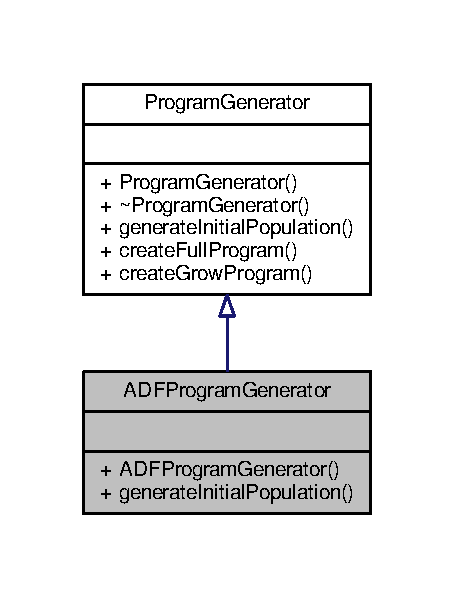
\includegraphics[width=218pt]{classADFProgramGenerator__inherit__graph}
\end{center}
\end{figure}


Collaboration diagram for A\+D\+F\+Program\+Generator\+:
\nopagebreak
\begin{figure}[H]
\begin{center}
\leavevmode
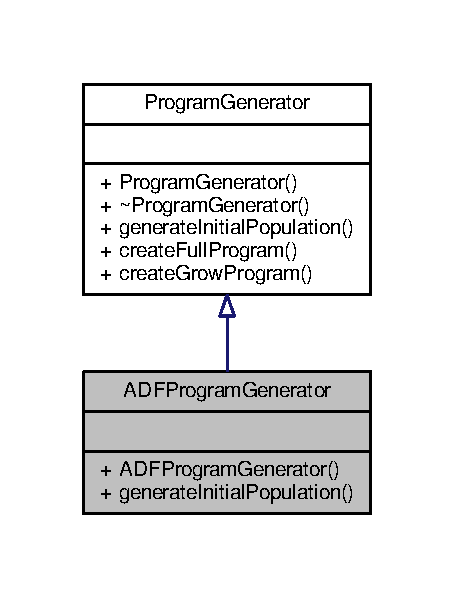
\includegraphics[width=218pt]{classADFProgramGenerator__coll__graph}
\end{center}
\end{figure}
\subsection*{Public Member Functions}
\begin{DoxyCompactItemize}
\item 
\hypertarget{classADFProgramGenerator_ae36a2f44de734a35861ce4480692902f}{}\label{classADFProgramGenerator_ae36a2f44de734a35861ce4480692902f} 
{\bfseries A\+D\+F\+Program\+Generator} (\hyperlink{classGPConfig}{G\+P\+Config} $\ast$)
\item 
\hypertarget{classADFProgramGenerator_ae5af12699c883fa26abc16861fae817d}{}\label{classADFProgramGenerator_ae5af12699c883fa26abc16861fae817d} 
virtual void {\bfseries generate\+Initial\+Population} (\hyperlink{classGeneticProgram}{Genetic\+Program} $\ast$pop\mbox{[}$\,$\mbox{]}, int num\+Individuals, int min\+Size, int max\+Size, int expected\+Size, int expected\+Return\+Type)
\end{DoxyCompactItemize}


The documentation for this class was generated from the following files\+:\begin{DoxyCompactItemize}
\item 
/home/\+Lach/npr-\/v109/\+R\+M\+I\+T\+G\+P.\+1.\+5/A\+D\+F\+Program\+Generator.\+h\item 
/home/\+Lach/npr-\/v109/\+R\+M\+I\+T\+G\+P.\+1.\+5/A\+D\+F\+Program\+Generator.\+cpp\end{DoxyCompactItemize}

\hypertarget{classADFRoot}{}\section{A\+D\+F\+Root Class Reference}
\label{classADFRoot}\index{A\+D\+F\+Root@{A\+D\+F\+Root}}


Inheritance diagram for A\+D\+F\+Root\+:
\nopagebreak
\begin{figure}[H]
\begin{center}
\leavevmode
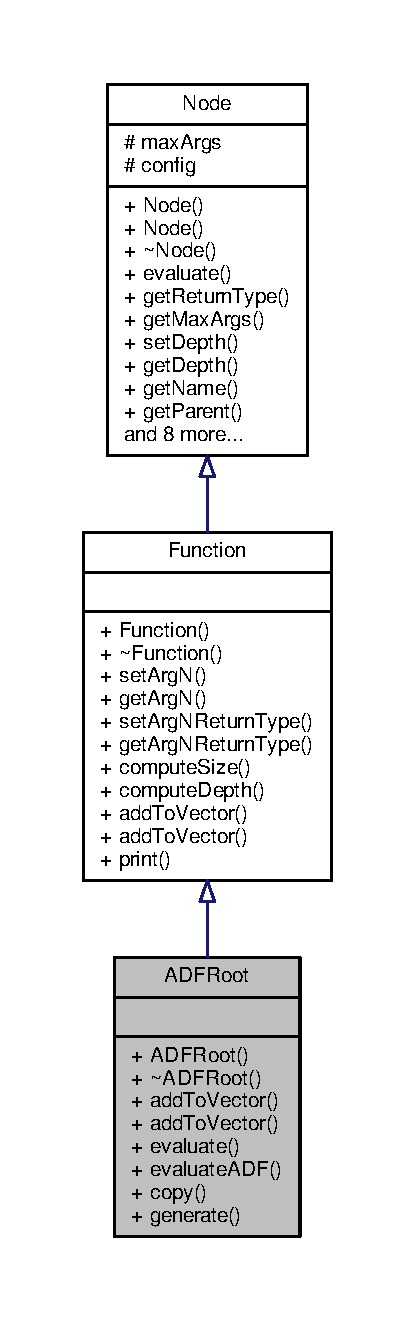
\includegraphics[height=550pt]{classADFRoot__inherit__graph}
\end{center}
\end{figure}


Collaboration diagram for A\+D\+F\+Root\+:
\nopagebreak
\begin{figure}[H]
\begin{center}
\leavevmode
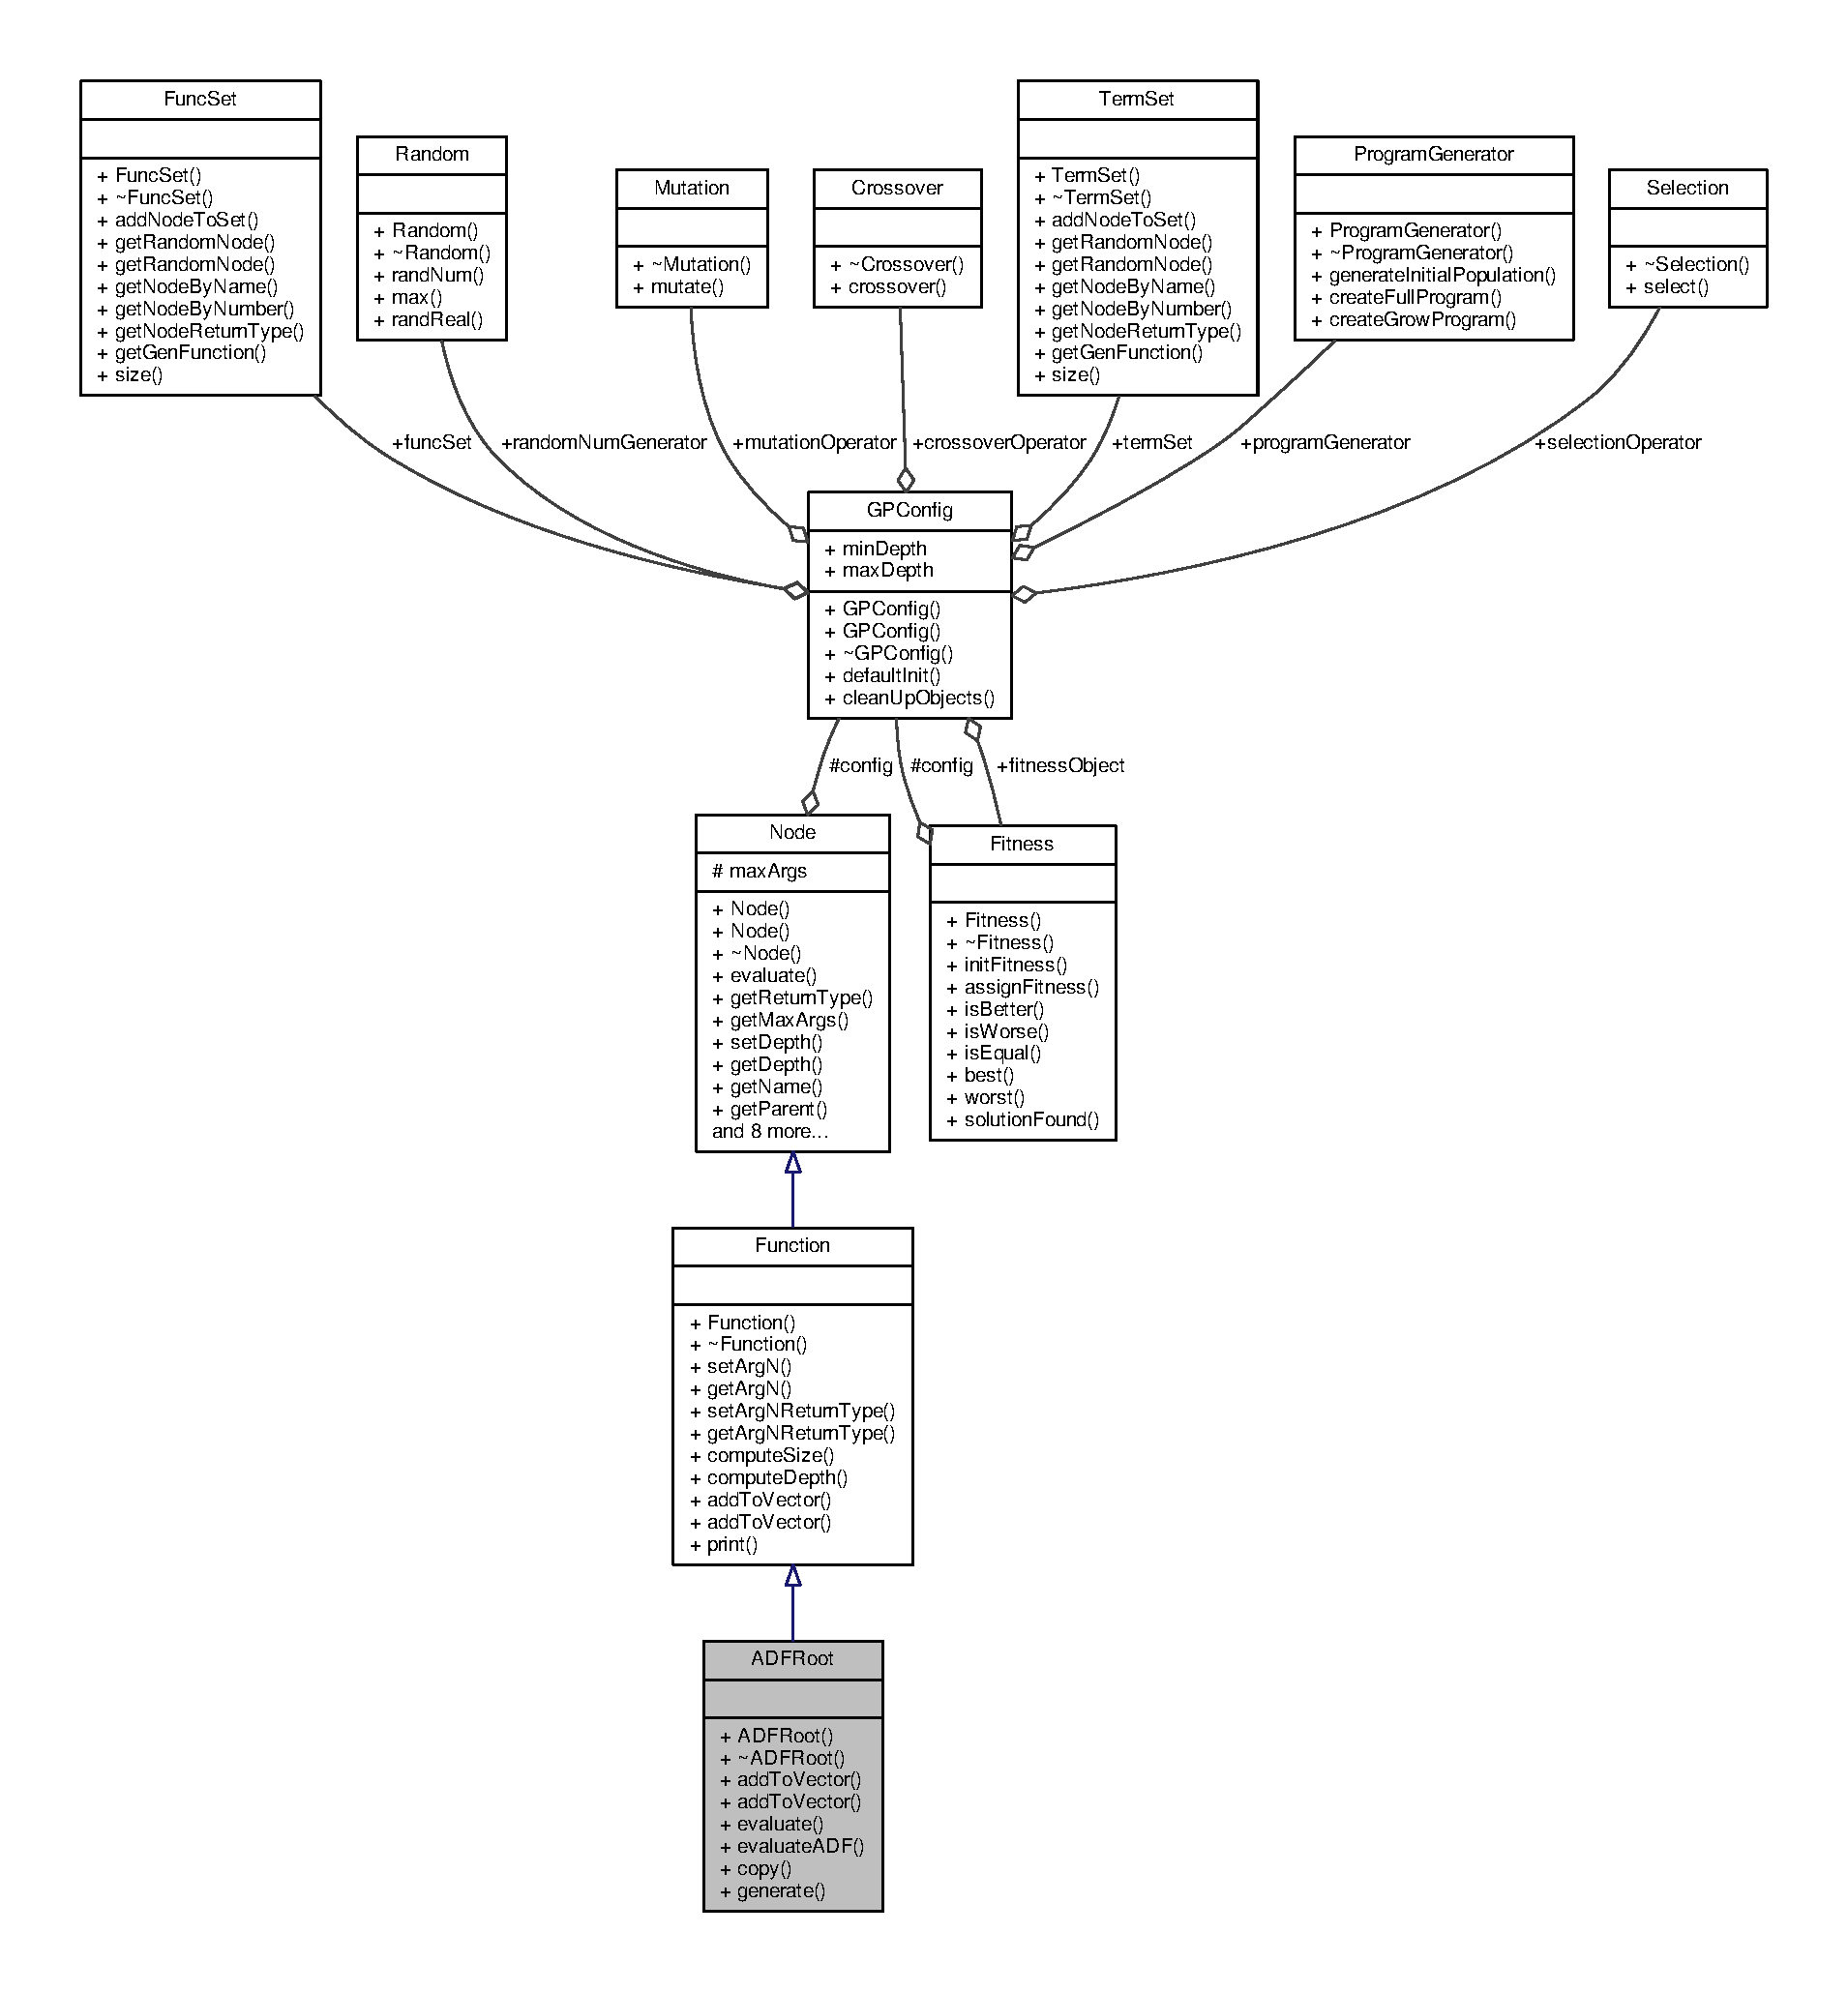
\includegraphics[width=350pt]{classADFRoot__coll__graph}
\end{center}
\end{figure}
\subsection*{Public Member Functions}
\begin{DoxyCompactItemize}
\item 
\hypertarget{classADFRoot_acde583cf9fe46ce521fcf856d3d4cc19}{}\label{classADFRoot_acde583cf9fe46ce521fcf856d3d4cc19} 
{\bfseries A\+D\+F\+Root} (\hyperlink{classGPConfig}{G\+P\+Config} $\ast$conf, int expected\+Return\+Type)
\item 
\hypertarget{classADFRoot_a50591f5fb63f6718e4a60fe24088c48f}{}\label{classADFRoot_a50591f5fb63f6718e4a60fe24088c48f} 
virtual void {\bfseries add\+To\+Vector} (vector$<$ \hyperlink{classNode}{Node} $\ast$$>$ \&vec)
\item 
\hypertarget{classADFRoot_acaffcb943d4f8a19bc679ee5534ffef3}{}\label{classADFRoot_acaffcb943d4f8a19bc679ee5534ffef3} 
virtual void {\bfseries add\+To\+Vector} (vector$<$ \hyperlink{classNode}{Node} $\ast$$>$ \&vec, int type\+Num)
\item 
\hypertarget{classADFRoot_a617d8b451f6b51f10270921ed2073f81}{}\label{classADFRoot_a617d8b451f6b51f10270921ed2073f81} 
virtual void {\bfseries evaluate} (\hyperlink{classReturnData}{Return\+Data} $\ast$out)
\item 
\hypertarget{classADFRoot_af88ef44b4fca614032d83981a5886ceb}{}\label{classADFRoot_af88ef44b4fca614032d83981a5886ceb} 
virtual void {\bfseries evaluate\+A\+DF} (\hyperlink{classReturnData}{Return\+Data} $\ast$out)
\item 
\hypertarget{classADFRoot_a7f76896e68d8004c8699b724af0fa9b1}{}\label{classADFRoot_a7f76896e68d8004c8699b724af0fa9b1} 
virtual \hyperlink{classNode}{Node} $\ast$ {\bfseries copy} ()
\end{DoxyCompactItemize}
\subsection*{Static Public Member Functions}
\begin{DoxyCompactItemize}
\item 
\hypertarget{classADFRoot_a1d825b0d257b308ed9b81f4d7ab4aa51}{}\label{classADFRoot_a1d825b0d257b308ed9b81f4d7ab4aa51} 
static \hyperlink{classFunction}{Function} $\ast$ {\bfseries generate} (const string \&name, \hyperlink{classGPConfig}{G\+P\+Config} $\ast$conf)
\end{DoxyCompactItemize}
\subsection*{Additional Inherited Members}


The documentation for this class was generated from the following files\+:\begin{DoxyCompactItemize}
\item 
/home/\+Lach/npr-\/v109/\+R\+M\+I\+T\+G\+P.\+1.\+5/A\+D\+F\+Root.\+h\item 
/home/\+Lach/npr-\/v109/\+R\+M\+I\+T\+G\+P.\+1.\+5/A\+D\+F\+Root.\+cpp\end{DoxyCompactItemize}

\hypertarget{classADFunction}{}\section{A\+D\+Function Class Reference}
\label{classADFunction}\index{A\+D\+Function@{A\+D\+Function}}


Inheritance diagram for A\+D\+Function\+:
\nopagebreak
\begin{figure}[H]
\begin{center}
\leavevmode
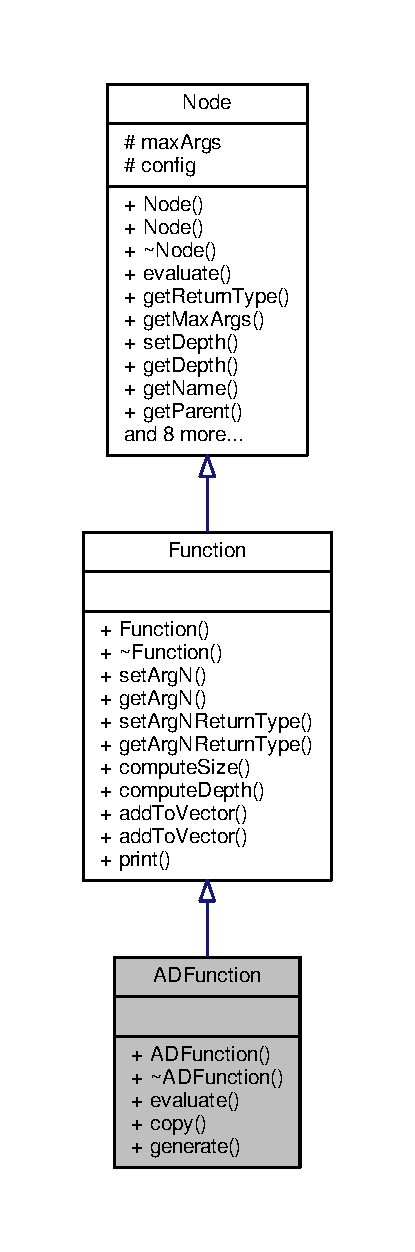
\includegraphics[height=550pt]{classADFunction__inherit__graph}
\end{center}
\end{figure}


Collaboration diagram for A\+D\+Function\+:
\nopagebreak
\begin{figure}[H]
\begin{center}
\leavevmode
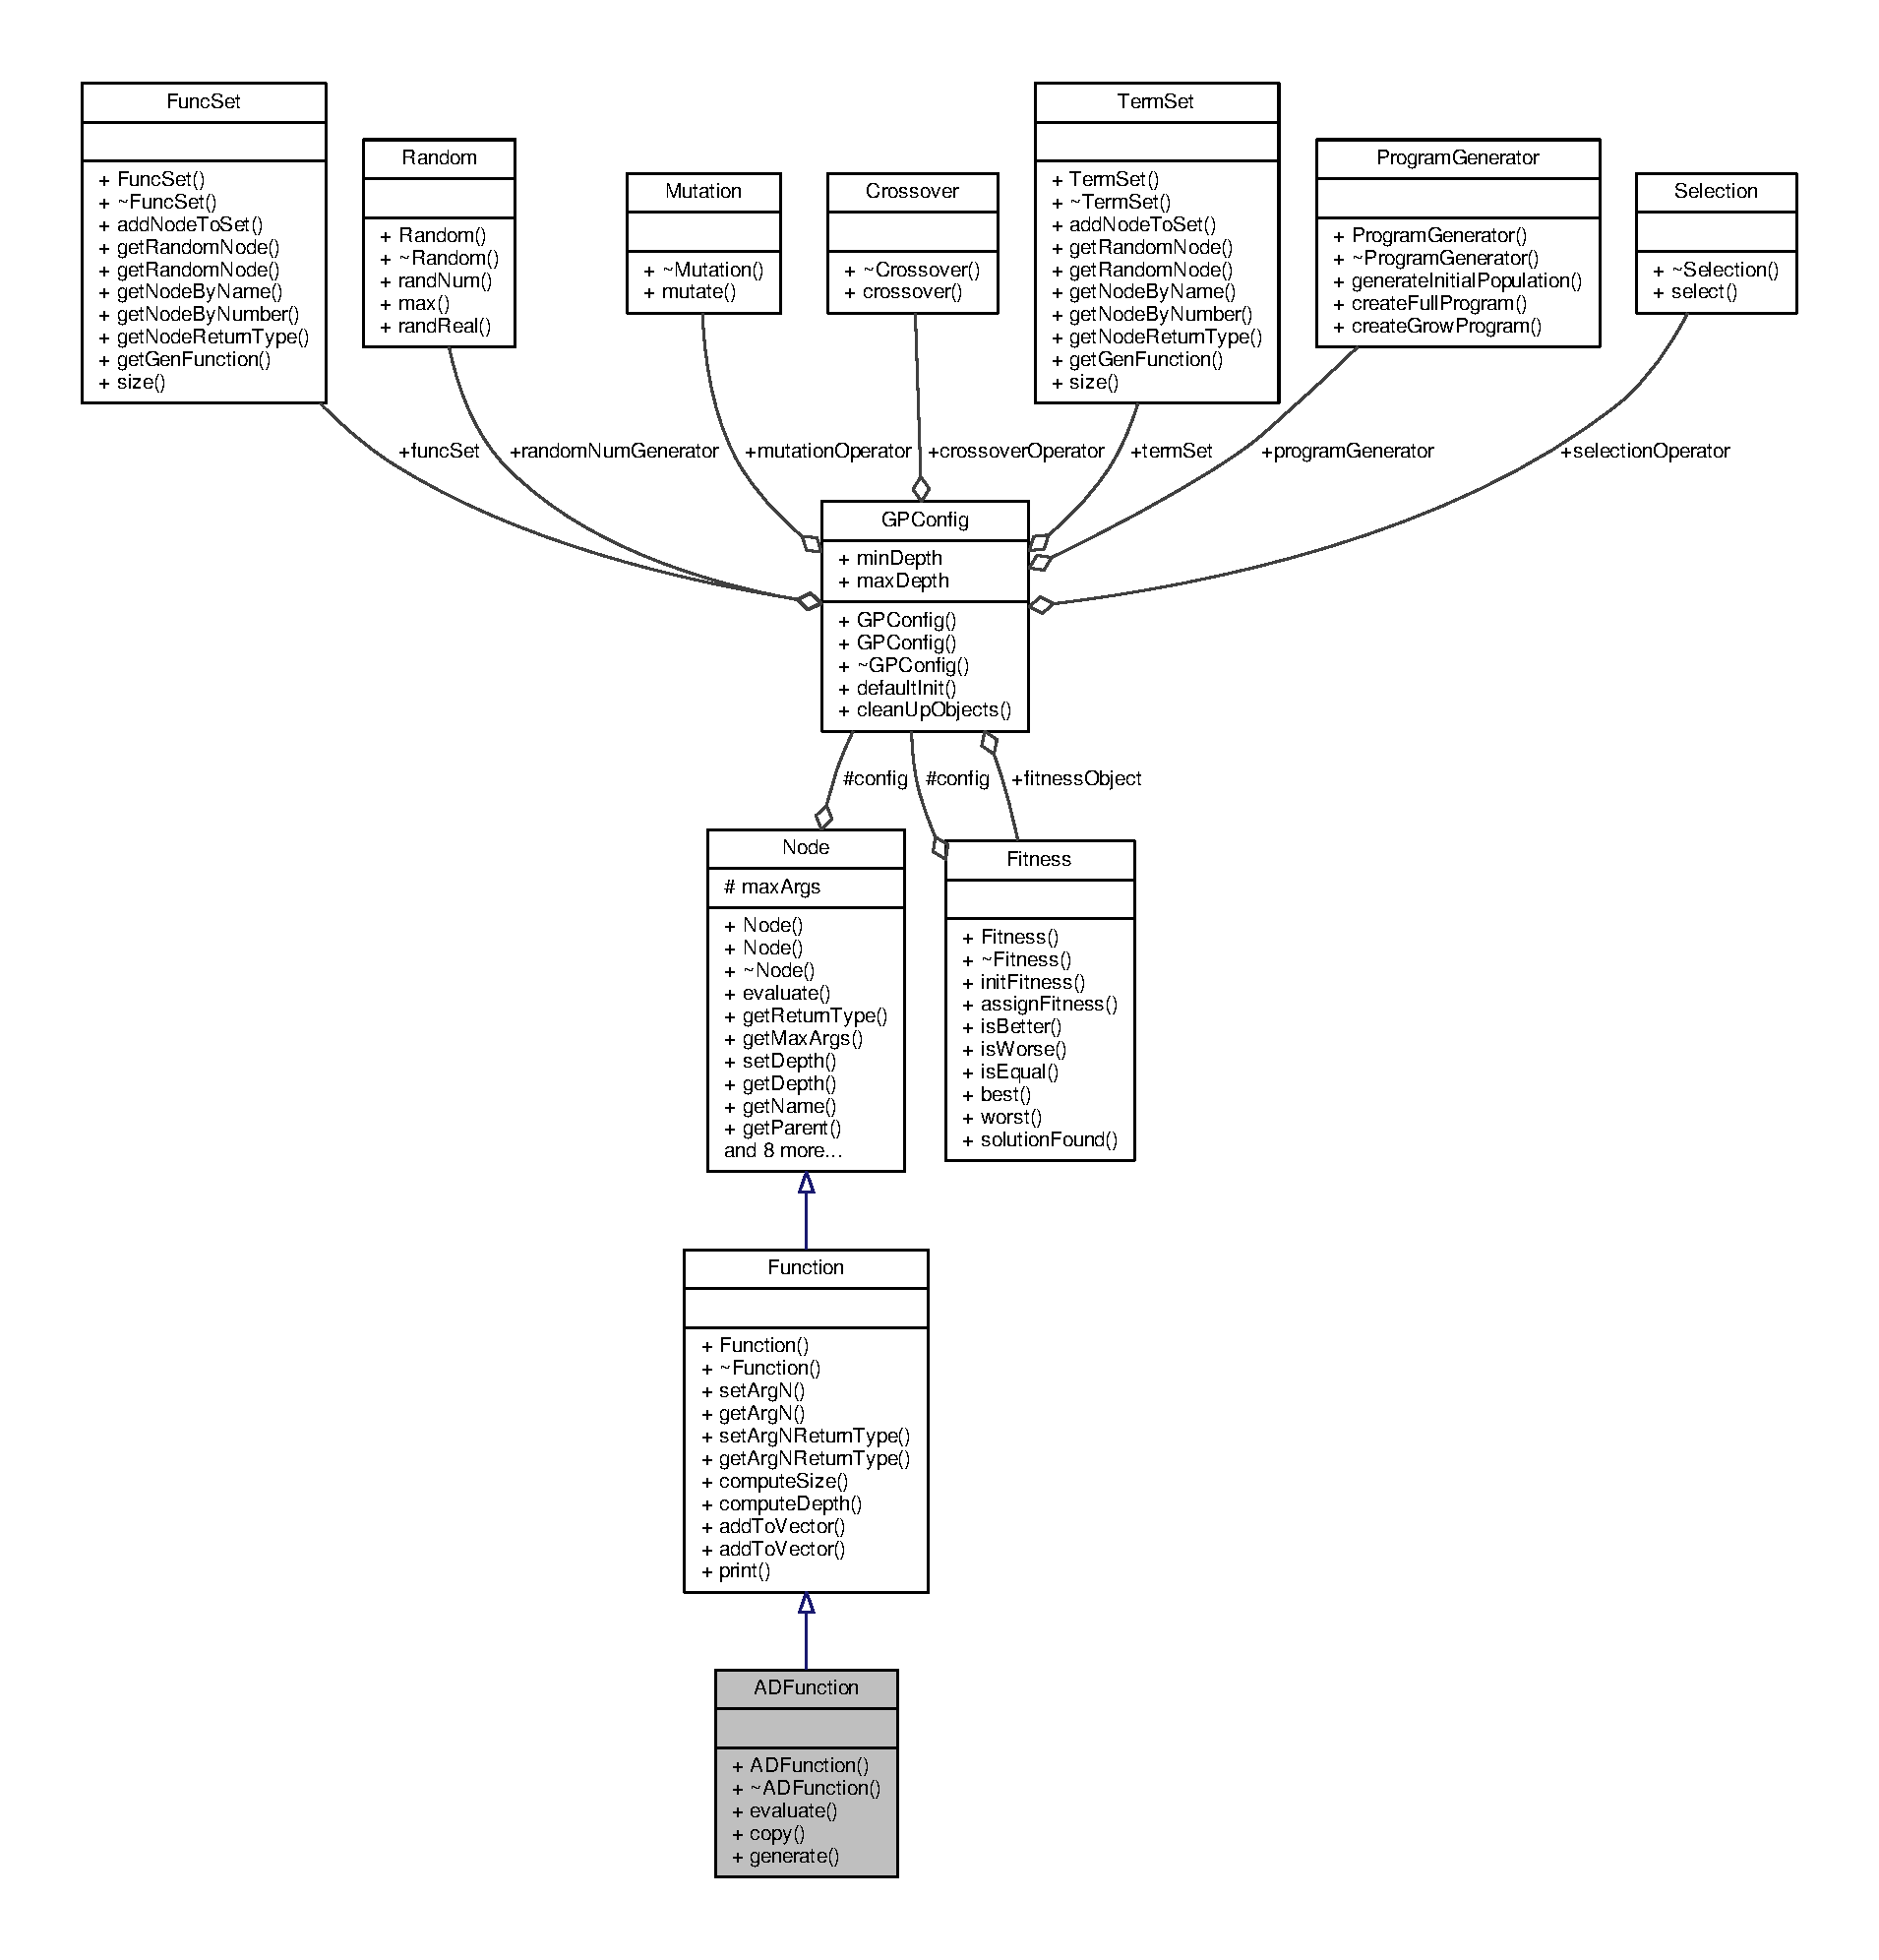
\includegraphics[width=350pt]{classADFunction__coll__graph}
\end{center}
\end{figure}
\subsection*{Public Member Functions}
\begin{DoxyCompactItemize}
\item 
\hypertarget{classADFunction_ac498ec67ffe4b56132621557f5acf44d}{}\label{classADFunction_ac498ec67ffe4b56132621557f5acf44d} 
{\bfseries A\+D\+Function} (\hyperlink{classGPConfig}{G\+P\+Config} $\ast$conf)
\item 
\hypertarget{classADFunction_a01062cbb089c4ef86091c0f6e4757649}{}\label{classADFunction_a01062cbb089c4ef86091c0f6e4757649} 
virtual void {\bfseries evaluate} (\hyperlink{classReturnData}{Return\+Data} $\ast$out)
\item 
\hypertarget{classADFunction_a1c23913e64d27ab6314617c35b9418b1}{}\label{classADFunction_a1c23913e64d27ab6314617c35b9418b1} 
virtual \hyperlink{classNode}{Node} $\ast$ {\bfseries copy} ()
\end{DoxyCompactItemize}
\subsection*{Static Public Member Functions}
\begin{DoxyCompactItemize}
\item 
\hypertarget{classADFunction_abd55170dadd403e819ad2d44ca699366}{}\label{classADFunction_abd55170dadd403e819ad2d44ca699366} 
static \hyperlink{classFunction}{Function} $\ast$ {\bfseries generate} (const string \&name, \hyperlink{classGPConfig}{G\+P\+Config} $\ast$conf)
\end{DoxyCompactItemize}
\subsection*{Additional Inherited Members}


The documentation for this class was generated from the following files\+:\begin{DoxyCompactItemize}
\item 
/home/\+Lach/npr-\/v109/\+R\+M\+I\+T\+G\+P.\+1.\+5/A\+D\+Function.\+h\item 
/home/\+Lach/npr-\/v109/\+R\+M\+I\+T\+G\+P.\+1.\+5/A\+D\+Function.\+cpp\end{DoxyCompactItemize}

\hypertarget{classBestCanvas}{}\section{Best\+Canvas Class Reference}
\label{classBestCanvas}\index{Best\+Canvas@{Best\+Canvas}}


Collaboration diagram for Best\+Canvas\+:
\nopagebreak
\begin{figure}[H]
\begin{center}
\leavevmode
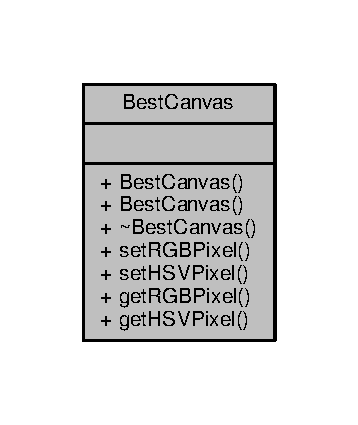
\includegraphics[width=172pt]{classBestCanvas__coll__graph}
\end{center}
\end{figure}
\subsection*{Public Member Functions}
\begin{DoxyCompactItemize}
\item 
\hypertarget{classBestCanvas_ad182d4690d4551842643aebecc7c4855}{}\label{classBestCanvas_ad182d4690d4551842643aebecc7c4855} 
{\bfseries Best\+Canvas} (\hyperlink{classTarget}{Target} $\ast$target, color\+\_\+t bg)
\item 
\hypertarget{classBestCanvas_a8fe1a93900c9c241d180cc4302724458}{}\label{classBestCanvas_a8fe1a93900c9c241d180cc4302724458} 
{\bfseries Best\+Canvas} (\hyperlink{classTarget}{Target} $\ast$target, color\+\_\+t bg\+\_\+\+Red, color\+\_\+t bg\+\_\+\+Green, color\+\_\+t bg\+\_\+\+Blue)
\item 
\hypertarget{classBestCanvas_a132c5ae0ba4a64d861e0f02f4318f4cb}{}\label{classBestCanvas_a132c5ae0ba4a64d861e0f02f4318f4cb} 
void {\bfseries set\+R\+G\+B\+Pixel} (int offset, \hyperlink{structRGB}{R\+GB} pixel)
\item 
\hypertarget{classBestCanvas_a596f525da74cfb4f889ceca87a9cf4f6}{}\label{classBestCanvas_a596f525da74cfb4f889ceca87a9cf4f6} 
void {\bfseries set\+H\+S\+V\+Pixel} (int offset, \hyperlink{structHSV}{H\+SV} pixel)
\item 
\hypertarget{classBestCanvas_abd9c06a1c0304bec04a5060f31f6d9b8}{}\label{classBestCanvas_abd9c06a1c0304bec04a5060f31f6d9b8} 
\hyperlink{structRGB}{R\+GB} {\bfseries get\+R\+G\+B\+Pixel} (\hyperlink{structCoord}{Coord} c)
\item 
\hypertarget{classBestCanvas_ae973df7ff7f90693cca4b883ccde1d59}{}\label{classBestCanvas_ae973df7ff7f90693cca4b883ccde1d59} 
\hyperlink{structHSV}{H\+SV} {\bfseries get\+H\+S\+V\+Pixel} (\hyperlink{structCoord}{Coord} c)
\end{DoxyCompactItemize}


The documentation for this class was generated from the following files\+:\begin{DoxyCompactItemize}
\item 
/home/\+Lach/npr-\/v109/src\+\_\+109/Best\+Canvas.\+h\item 
/home/\+Lach/npr-\/v109/src\+\_\+109/Best\+Canvas.\+cpp\end{DoxyCompactItemize}

\hypertarget{classBezierPathCanvas}{}\section{Bezier\+Path\+Canvas Class Reference}
\label{classBezierPathCanvas}\index{Bezier\+Path\+Canvas@{Bezier\+Path\+Canvas}}


Inheritance diagram for Bezier\+Path\+Canvas\+:
\nopagebreak
\begin{figure}[H]
\begin{center}
\leavevmode
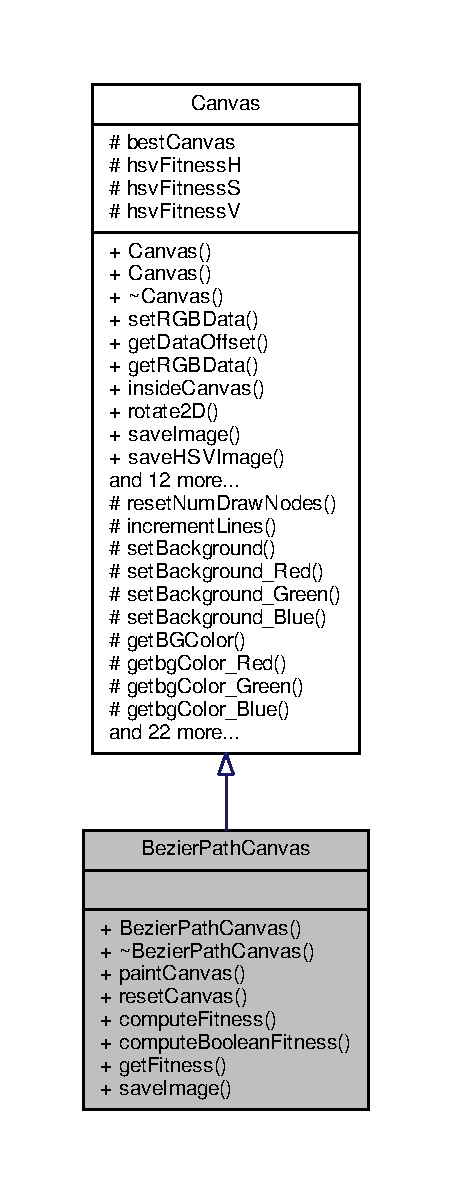
\includegraphics[height=550pt]{classBezierPathCanvas__inherit__graph}
\end{center}
\end{figure}


Collaboration diagram for Bezier\+Path\+Canvas\+:
\nopagebreak
\begin{figure}[H]
\begin{center}
\leavevmode
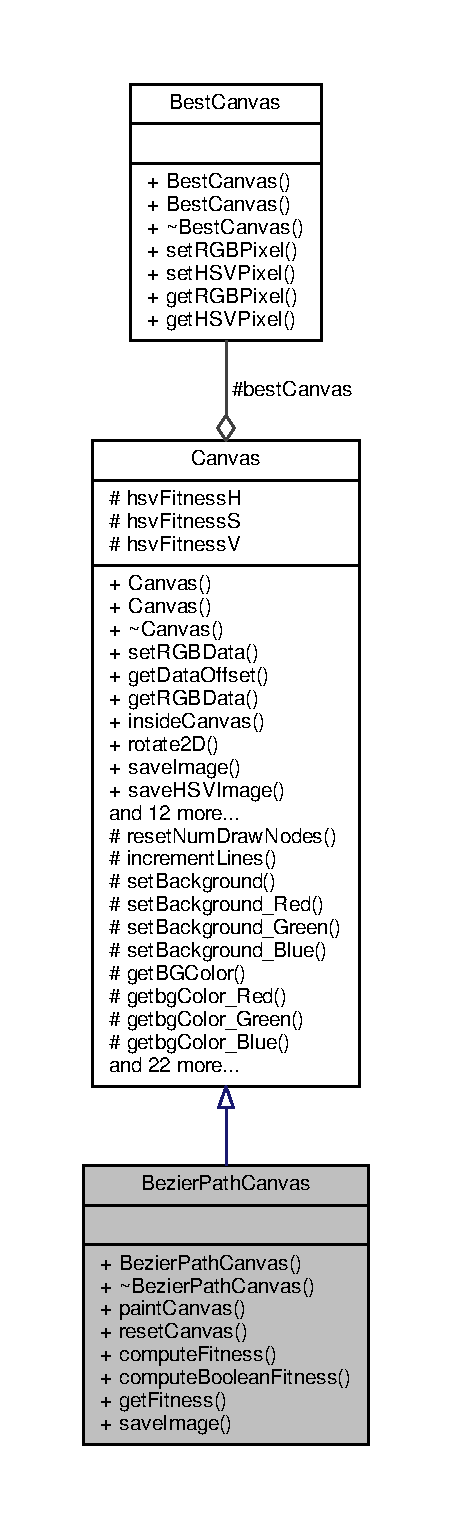
\includegraphics[height=550pt]{classBezierPathCanvas__coll__graph}
\end{center}
\end{figure}
\subsection*{Public Member Functions}
\begin{DoxyCompactItemize}
\item 
\hypertarget{classBezierPathCanvas_ae24f243f5019dbd8fcab3312ffbf1188}{}\label{classBezierPathCanvas_ae24f243f5019dbd8fcab3312ffbf1188} 
{\bfseries Bezier\+Path\+Canvas} (\hyperlink{classTarget}{Target} $\ast$t, color\+\_\+t bg, \hyperlink{classBestCanvas}{Best\+Canvas} $\ast$bc, \hyperlink{classConfigReader}{Config\+Reader} $\ast$reader)
\item 
\hypertarget{classBezierPathCanvas_a416fa47f6b5cdac2bfb97851da5d14f7}{}\label{classBezierPathCanvas_a416fa47f6b5cdac2bfb97851da5d14f7} 
void {\bfseries paint\+Canvas} (vector$<$ float $>$)
\item 
\hypertarget{classBezierPathCanvas_a9cbaaad5348b95398638c82e899603d6}{}\label{classBezierPathCanvas_a9cbaaad5348b95398638c82e899603d6} 
void {\bfseries reset\+Canvas} ()
\item 
\hypertarget{classBezierPathCanvas_a2262510eb3b0f95754b10c6baae55373}{}\label{classBezierPathCanvas_a2262510eb3b0f95754b10c6baae55373} 
void {\bfseries compute\+Fitness} ()
\item 
\hypertarget{classBezierPathCanvas_a5c875f0efc1936e6d87b32a4846ff890}{}\label{classBezierPathCanvas_a5c875f0efc1936e6d87b32a4846ff890} 
void {\bfseries compute\+Boolean\+Fitness} ()
\item 
\hypertarget{classBezierPathCanvas_a2baf50cc95bdf9a2de442ae38bb586fb}{}\label{classBezierPathCanvas_a2baf50cc95bdf9a2de442ae38bb586fb} 
float {\bfseries get\+Fitness} ()
\item 
\hypertarget{classBezierPathCanvas_a4f96f789b6ab895d3efb05fd6de199d6}{}\label{classBezierPathCanvas_a4f96f789b6ab895d3efb05fd6de199d6} 
bool {\bfseries save\+Image} (char $\ast$filename)
\end{DoxyCompactItemize}
\subsection*{Additional Inherited Members}


The documentation for this class was generated from the following files\+:\begin{DoxyCompactItemize}
\item 
/home/\+Lach/npr-\/v109/src\+\_\+109/Bezier\+Path\+Canvas.\+h\item 
/home/\+Lach/npr-\/v109/src\+\_\+109/Bezier\+Path\+Canvas.\+cpp\end{DoxyCompactItemize}

\hypertarget{classCanny}{}\section{Canny Class Reference}
\label{classCanny}\index{Canny@{Canny}}


Collaboration diagram for Canny\+:
\nopagebreak
\begin{figure}[H]
\begin{center}
\leavevmode
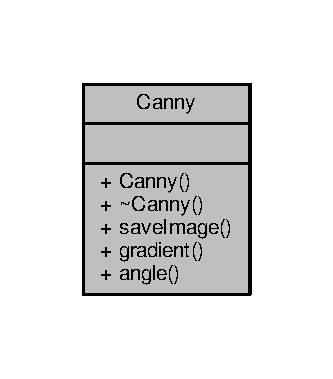
\includegraphics[width=160pt]{classCanny__coll__graph}
\end{center}
\end{figure}
\subsection*{Public Member Functions}
\begin{DoxyCompactItemize}
\item 
\hypertarget{classCanny_a1ad410465ac8ce1297e2b2da3af251a4}{}\label{classCanny_a1ad410465ac8ce1297e2b2da3af251a4} 
{\bfseries Canny} (\hyperlink{structRGB}{R\+GB} $\ast$rgb, int width, int height, int t1, int t2, bool fuzzy\+Edges)
\item 
\hypertarget{classCanny_ae55fb997a745394d6a458ff2614d96bc}{}\label{classCanny_ae55fb997a745394d6a458ff2614d96bc} 
bool {\bfseries save\+Image} (std\+::string filename)
\item 
\hypertarget{classCanny_a8ed16206ee4a1e2b83bc044c6ea44edf}{}\label{classCanny_a8ed16206ee4a1e2b83bc044c6ea44edf} 
color\+\_\+t {\bfseries gradient} (\hyperlink{structCoord}{Coord} c)
\item 
\hypertarget{classCanny_ad772d59de68ce90791123e51f32b76d8}{}\label{classCanny_ad772d59de68ce90791123e51f32b76d8} 
float {\bfseries angle} (\hyperlink{structCoord}{Coord} c)
\end{DoxyCompactItemize}


The documentation for this class was generated from the following files\+:\begin{DoxyCompactItemize}
\item 
/home/\+Lach/npr-\/v109/src\+\_\+109/Canny.\+h\item 
/home/\+Lach/npr-\/v109/src\+\_\+109/Canny.\+cpp\end{DoxyCompactItemize}

\hypertarget{classCanvas}{}\section{Canvas Class Reference}
\label{classCanvas}\index{Canvas@{Canvas}}


Inheritance diagram for Canvas\+:
\nopagebreak
\begin{figure}[H]
\begin{center}
\leavevmode
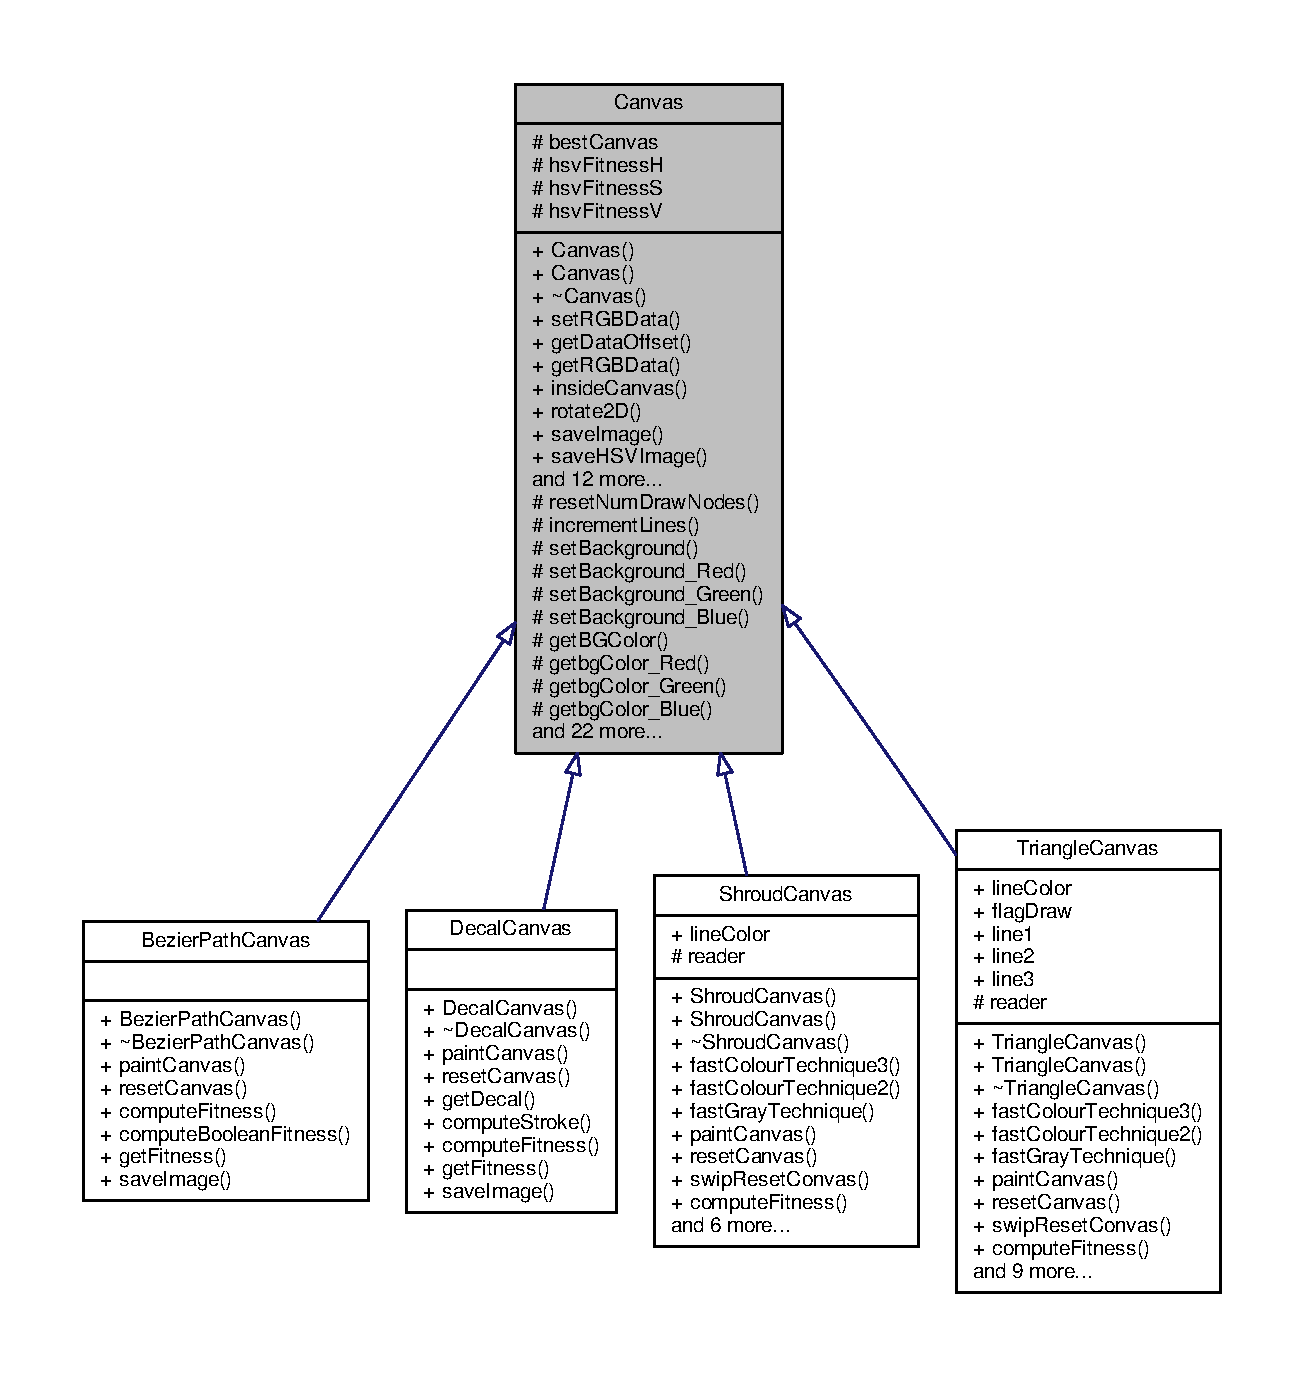
\includegraphics[width=350pt]{classCanvas__inherit__graph}
\end{center}
\end{figure}


Collaboration diagram for Canvas\+:
\nopagebreak
\begin{figure}[H]
\begin{center}
\leavevmode
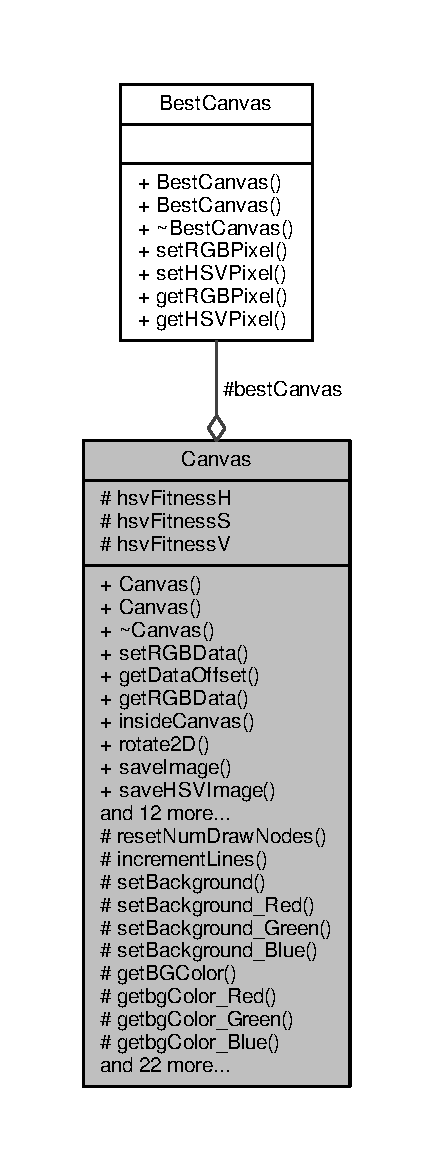
\includegraphics[height=550pt]{classCanvas__coll__graph}
\end{center}
\end{figure}
\subsection*{Public Member Functions}
\begin{DoxyCompactItemize}
\item 
\hypertarget{classCanvas_a53b246273af5f8312e98963ebc5f18c8}{}\label{classCanvas_a53b246273af5f8312e98963ebc5f18c8} 
{\bfseries Canvas} (\hyperlink{classTarget}{Target} $\ast$t, color\+\_\+t bg, \hyperlink{classBestCanvas}{Best\+Canvas} $\ast$bc)
\item 
\hypertarget{classCanvas_ae3d42b2fc30548f6c6bf7d269067e9c7}{}\label{classCanvas_ae3d42b2fc30548f6c6bf7d269067e9c7} 
{\bfseries Canvas} (\hyperlink{classTarget}{Target} $\ast$t, color\+\_\+t bg\+\_\+\+Red, color\+\_\+t bg\+\_\+\+Green, color\+\_\+t bg\+\_\+\+Blue, \hyperlink{classBestCanvas}{Best\+Canvas} $\ast$bc)
\item 
virtual \hyperlink{classCanvas_a237c4549ad2e27c729cd1f71e89f0fd9}{$\sim$\+Canvas} ()
\item 
\hypertarget{classCanvas_aa6fd94baa21ffded183b4bf2375d9516}{}\label{classCanvas_aa6fd94baa21ffded183b4bf2375d9516} 
void {\bfseries set\+R\+G\+B\+Data} (int offset, \hyperlink{structRGB}{R\+GB} pixel)
\item 
\hypertarget{classCanvas_a9b47997839f63bda394c7385eac6f96e}{}\label{classCanvas_a9b47997839f63bda394c7385eac6f96e} 
const int {\bfseries get\+Data\+Offset} (\hyperlink{structCoord}{Coord} c)
\item 
\hypertarget{classCanvas_ab1686ad837e67a4c93d7539d0d3d0151}{}\label{classCanvas_ab1686ad837e67a4c93d7539d0d3d0151} 
\hyperlink{structRGB}{R\+GB} {\bfseries get\+R\+G\+B\+Data} (int offset)
\item 
\hypertarget{classCanvas_a9e51f90be565cb3e5d683cdf83d67956}{}\label{classCanvas_a9e51f90be565cb3e5d683cdf83d67956} 
bool {\bfseries inside\+Canvas} (\hyperlink{structCoord}{Coord})
\item 
\hypertarget{classCanvas_ae397083afa0345eec9c0e212903a6394}{}\label{classCanvas_ae397083afa0345eec9c0e212903a6394} 
\hyperlink{structCoord}{Coord} {\bfseries rotate2D} (\hyperlink{structCoord}{Coord} c, float dx, float dy, float theta)
\item 
\hypertarget{classCanvas_abbde1d2cfe76cb174828233e610b62ac}{}\label{classCanvas_abbde1d2cfe76cb174828233e610b62ac} 
virtual bool {\bfseries save\+Image} (char $\ast$filename)=0
\item 
\hypertarget{classCanvas_a20a5bfc766b35f031f87602a33d004b1}{}\label{classCanvas_a20a5bfc766b35f031f87602a33d004b1} 
bool {\bfseries save\+H\+S\+V\+Image} (char $\ast$filename)
\item 
\hypertarget{classCanvas_a0cd8a0f0e6a1b8bae854d93277926951}{}\label{classCanvas_a0cd8a0f0e6a1b8bae854d93277926951} 
bool {\bfseries save\+R\+G\+B\+Image} (char $\ast$filename)
\item 
\hypertarget{classCanvas_abd119da0a1dc1b24a45c8c45bd398732}{}\label{classCanvas_abd119da0a1dc1b24a45c8c45bd398732} 
virtual void {\bfseries reset\+Canvas} ()=0
\item 
\hypertarget{classCanvas_aa5c92419e72221fd67fae506419ec165}{}\label{classCanvas_aa5c92419e72221fd67fae506419ec165} 
virtual void {\bfseries paint\+Canvas} (vector$<$ float $>$)=0
\item 
\hypertarget{classCanvas_a23c0eb700982cfb7e8f468b51aa7adde}{}\label{classCanvas_a23c0eb700982cfb7e8f468b51aa7adde} 
int {\bfseries get\+Num\+Draw\+Nodes} ()
\item 
\hypertarget{classCanvas_a9a96d277519345b76e27349ca8d6421d}{}\label{classCanvas_a9a96d277519345b76e27349ca8d6421d} 
virtual void {\bfseries compute\+Fitness} ()=0
\item 
\hypertarget{classCanvas_a21fb2ed04cb521a5cdb3516bfa7bf6f1}{}\label{classCanvas_a21fb2ed04cb521a5cdb3516bfa7bf6f1} 
virtual float {\bfseries get\+Fitness} ()=0
\item 
\hypertarget{classCanvas_af78dc240a3278b5d7abad1cd743e31c4}{}\label{classCanvas_af78dc240a3278b5d7abad1cd743e31c4} 
const int {\bfseries get\+Size} ()
\item 
\hypertarget{classCanvas_a32c661c9bf432d32b6b75d097cba614f}{}\label{classCanvas_a32c661c9bf432d32b6b75d097cba614f} 
bool {\bfseries pixel\+Is\+Dirty} (\hyperlink{structCoord}{Coord} c)
\item 
\hypertarget{classCanvas_aff7ccbf887a62cfaf2785845d5dabb17}{}\label{classCanvas_aff7ccbf887a62cfaf2785845d5dabb17} 
bool {\bfseries pixel\+Is\+White} (\hyperlink{structCoord}{Coord} c)
\item 
\hypertarget{classCanvas_ac2032301cc13268992ecf3df85b73de0}{}\label{classCanvas_ac2032301cc13268992ecf3df85b73de0} 
void {\bfseries update\+Best\+Canvas} ()
\item 
\hypertarget{classCanvas_a36f33f02cee811e0d5a13e659eeb1f73}{}\label{classCanvas_a36f33f02cee811e0d5a13e659eeb1f73} 
const int {\bfseries get\+Width} ()
\item 
\hypertarget{classCanvas_a0b94a41db3014f125219155940437505}{}\label{classCanvas_a0b94a41db3014f125219155940437505} 
const int {\bfseries get\+Height} ()
\end{DoxyCompactItemize}
\subsection*{Protected Member Functions}
\begin{DoxyCompactItemize}
\item 
\hypertarget{classCanvas_a6740306cd9f07901b2bc31c2d4bbc3a3}{}\label{classCanvas_a6740306cd9f07901b2bc31c2d4bbc3a3} 
void {\bfseries reset\+Num\+Draw\+Nodes} ()
\item 
\hypertarget{classCanvas_a9381d59bc23a115890fda270eecc69f1}{}\label{classCanvas_a9381d59bc23a115890fda270eecc69f1} 
void {\bfseries increment\+Lines} ()
\item 
\hypertarget{classCanvas_a0227884bab636ac95308b239c99f3466}{}\label{classCanvas_a0227884bab636ac95308b239c99f3466} 
void {\bfseries set\+Background} (color\+\_\+t bg)
\item 
\hypertarget{classCanvas_abf204df96ee5233c09817245942a52f5}{}\label{classCanvas_abf204df96ee5233c09817245942a52f5} 
void {\bfseries set\+Background\+\_\+\+Red} (color\+\_\+t bg)
\item 
\hypertarget{classCanvas_aacbfeb32c1611636b937d9eddc6042f0}{}\label{classCanvas_aacbfeb32c1611636b937d9eddc6042f0} 
void {\bfseries set\+Background\+\_\+\+Green} (color\+\_\+t bg)
\item 
\hypertarget{classCanvas_a447151f796bafcbd3cbbc5191d98aa40}{}\label{classCanvas_a447151f796bafcbd3cbbc5191d98aa40} 
void {\bfseries set\+Background\+\_\+\+Blue} (color\+\_\+t bg)
\item 
\hypertarget{classCanvas_a24ccd2a00993f23addb6b29080a9733a}{}\label{classCanvas_a24ccd2a00993f23addb6b29080a9733a} 
const color\+\_\+t {\bfseries get\+B\+G\+Color} ()
\item 
\hypertarget{classCanvas_a71cfe236e024ae60ac8941cca8f1eb7a}{}\label{classCanvas_a71cfe236e024ae60ac8941cca8f1eb7a} 
const color\+\_\+t {\bfseries getbg\+Color\+\_\+\+Red} ()
\item 
\hypertarget{classCanvas_a8d10f424606d7ac03bdb1197bd23742c}{}\label{classCanvas_a8d10f424606d7ac03bdb1197bd23742c} 
const color\+\_\+t {\bfseries getbg\+Color\+\_\+\+Green} ()
\item 
\hypertarget{classCanvas_a62e8cb7b9c0a99b64adda7ff5330e5a2}{}\label{classCanvas_a62e8cb7b9c0a99b64adda7ff5330e5a2} 
const color\+\_\+t {\bfseries getbg\+Color\+\_\+\+Blue} ()
\item 
\hypertarget{classCanvas_a2b7899e3b8ff4d9938b1b385011ccb25}{}\label{classCanvas_a2b7899e3b8ff4d9938b1b385011ccb25} 
\hyperlink{classTarget}{Target} $\ast$ {\bfseries get\+Target} ()
\item 
\hypertarget{classCanvas_acb06d2e4116994f32121333e69585249}{}\label{classCanvas_acb06d2e4116994f32121333e69585249} 
\hyperlink{structHSV}{H\+SV} {\bfseries get\+H\+S\+V\+Data} (int offset)
\item 
\hypertarget{classCanvas_a7fba7a894a1857c9ee2fe34441629d52}{}\label{classCanvas_a7fba7a894a1857c9ee2fe34441629d52} 
void {\bfseries set\+H\+S\+V\+Data} (int offset, \hyperlink{structHSV}{H\+SV} pixel)
\item 
\hypertarget{classCanvas_a8a7184ebaa6704048362972407787a59}{}\label{classCanvas_a8a7184ebaa6704048362972407787a59} 
void {\bfseries set\+H\+S\+V\+FitnessH} (float f)
\item 
\hypertarget{classCanvas_aa4e1c90061a6814daf5bbca65e1e398a}{}\label{classCanvas_aa4e1c90061a6814daf5bbca65e1e398a} 
void {\bfseries set\+H\+S\+V\+FitnessS} (float f)
\item 
\hypertarget{classCanvas_a068052d242a5c21a89b334224a127d19}{}\label{classCanvas_a068052d242a5c21a89b334224a127d19} 
void {\bfseries set\+H\+S\+V\+FitnessV} (float f)
\item 
\hypertarget{classCanvas_aa0c60ed66fcea208c32a2e3c8bf28923}{}\label{classCanvas_aa0c60ed66fcea208c32a2e3c8bf28923} 
int {\bfseries degrees\+Of\+Separation} (int, int)
\item 
\hypertarget{classCanvas_a56ba128080bcc03c8bb8b7d6c2cc9821}{}\label{classCanvas_a56ba128080bcc03c8bb8b7d6c2cc9821} 
void {\bfseries print\+Color} (\hyperlink{structRGB}{R\+GB} color)
\item 
\hypertarget{classCanvas_a570498c742d3e171b7be1c498f0e75f1}{}\label{classCanvas_a570498c742d3e171b7be1c498f0e75f1} 
void {\bfseries print\+Color} (\hyperlink{structHSV}{H\+SV} color)
\item 
\hypertarget{classCanvas_a95ecf73c2b84c001d12bc6dc6940091e}{}\label{classCanvas_a95ecf73c2b84c001d12bc6dc6940091e} 
\hyperlink{structRGB}{R\+GB} {\bfseries target\+Pixel\+R\+GB} (\hyperlink{structCoord}{Coord} c)
\item 
\hypertarget{classCanvas_a04b66e5e405d8785984a01d7b8dc639c}{}\label{classCanvas_a04b66e5e405d8785984a01d7b8dc639c} 
\hyperlink{structHSV}{H\+SV} {\bfseries target\+Pixel\+H\+SV} (\hyperlink{structCoord}{Coord} c)
\item 
\hypertarget{classCanvas_aa8c5064fd62e3aa1fde2bf94b806281e}{}\label{classCanvas_aa8c5064fd62e3aa1fde2bf94b806281e} 
int {\bfseries target\+Hue} (\hyperlink{structCoord}{Coord} c)
\item 
\hypertarget{classCanvas_aca87eeb2759686e9f9d1f28d9716393a}{}\label{classCanvas_aca87eeb2759686e9f9d1f28d9716393a} 
int {\bfseries target\+Sat} (\hyperlink{structCoord}{Coord} c)
\item 
\hypertarget{classCanvas_a69e2bd44307edae0ac346fefb80be422}{}\label{classCanvas_a69e2bd44307edae0ac346fefb80be422} 
int {\bfseries target\+Val} (\hyperlink{structCoord}{Coord} c)
\item 
\hypertarget{classCanvas_a13059f62106ec98aa56042e053a9d00a}{}\label{classCanvas_a13059f62106ec98aa56042e053a9d00a} 
int {\bfseries target\+Sat\+Gradient} (\hyperlink{structCoord}{Coord} c)
\item 
\hypertarget{classCanvas_a6f9d4ad8953ce2e7294e7ef611dcc7da}{}\label{classCanvas_a6f9d4ad8953ce2e7294e7ef611dcc7da} 
int {\bfseries target\+Val\+Gradient} (\hyperlink{structCoord}{Coord} c)
\item 
\hypertarget{classCanvas_a70268f85eead1127cffba07515ebc777}{}\label{classCanvas_a70268f85eead1127cffba07515ebc777} 
float {\bfseries target\+Sat\+Direction} (\hyperlink{structCoord}{Coord} c)
\item 
\hypertarget{classCanvas_ab8fe4798eaa8d2f630622b0a92664c25}{}\label{classCanvas_ab8fe4798eaa8d2f630622b0a92664c25} 
float {\bfseries target\+Val\+Direction} (\hyperlink{structCoord}{Coord} c)
\item 
\hypertarget{classCanvas_a467ca92f410dfb513f0cb6ab6fddcb9b}{}\label{classCanvas_a467ca92f410dfb513f0cb6ab6fddcb9b} 
int {\bfseries match\+Hue} (\hyperlink{structCoord}{Coord} c, int h)
\item 
\hypertarget{classCanvas_a51a62303ba86699a047c9b82151cc851}{}\label{classCanvas_a51a62303ba86699a047c9b82151cc851} 
int {\bfseries match\+Sat} (\hyperlink{structCoord}{Coord} c, int s)
\item 
\hypertarget{classCanvas_ab6c6ee4bb92793b61b4c99b64e3e4514}{}\label{classCanvas_ab6c6ee4bb92793b61b4c99b64e3e4514} 
int {\bfseries match\+Val} (\hyperlink{structCoord}{Coord} c, int v)
\item 
\hypertarget{classCanvas_a25fc15e87b8526fd411e227bfe94d1ca}{}\label{classCanvas_a25fc15e87b8526fd411e227bfe94d1ca} 
void {\bfseries compute\+H\+S\+V\+Fitness} ()
\end{DoxyCompactItemize}
\subsection*{Protected Attributes}
\begin{DoxyCompactItemize}
\item 
\hypertarget{classCanvas_a93c8956f408b11c81073f5d748a8e3b3}{}\label{classCanvas_a93c8956f408b11c81073f5d748a8e3b3} 
\hyperlink{classBestCanvas}{Best\+Canvas} $\ast$ {\bfseries best\+Canvas}
\item 
\hypertarget{classCanvas_aeff1549bc9fb9469f68227dbbee4a4de}{}\label{classCanvas_aeff1549bc9fb9469f68227dbbee4a4de} 
float {\bfseries hsv\+FitnessH}
\item 
\hypertarget{classCanvas_af04ba6d3e079fa937575f7ef80bfac6d}{}\label{classCanvas_af04ba6d3e079fa937575f7ef80bfac6d} 
float {\bfseries hsv\+FitnessS}
\item 
\hypertarget{classCanvas_a16bfdb1b384498d5aa0cbd674c6abfe4}{}\label{classCanvas_a16bfdb1b384498d5aa0cbd674c6abfe4} 
float {\bfseries hsv\+FitnessV}
\end{DoxyCompactItemize}


\subsection{Constructor \& Destructor Documentation}
\hypertarget{classCanvas_a237c4549ad2e27c729cd1f71e89f0fd9}{}\label{classCanvas_a237c4549ad2e27c729cd1f71e89f0fd9} 
\index{Canvas@{Canvas}!````~Canvas@{$\sim$\+Canvas}}
\index{````~Canvas@{$\sim$\+Canvas}!Canvas@{Canvas}}
\subsubsection{\texorpdfstring{$\sim$\+Canvas()}{~Canvas()}}
{\footnotesize\ttfamily Canvas\+::$\sim$\+Canvas (\begin{DoxyParamCaption}{ }\end{DoxyParamCaption})\hspace{0.3cm}{\ttfamily [virtual]}}

Canvas\+::\+Canvas() \{ \} 

The documentation for this class was generated from the following files\+:\begin{DoxyCompactItemize}
\item 
/home/\+Lach/npr-\/v109/src\+\_\+109/Canvas.\+h\item 
/home/\+Lach/npr-\/v109/src\+\_\+109/Canvas.\+cpp\end{DoxyCompactItemize}

\hypertarget{classCoEvolutionFitness}{}\section{Co\+Evolution\+Fitness Class Reference}
\label{classCoEvolutionFitness}\index{Co\+Evolution\+Fitness@{Co\+Evolution\+Fitness}}


Inheritance diagram for Co\+Evolution\+Fitness\+:
\nopagebreak
\begin{figure}[H]
\begin{center}
\leavevmode
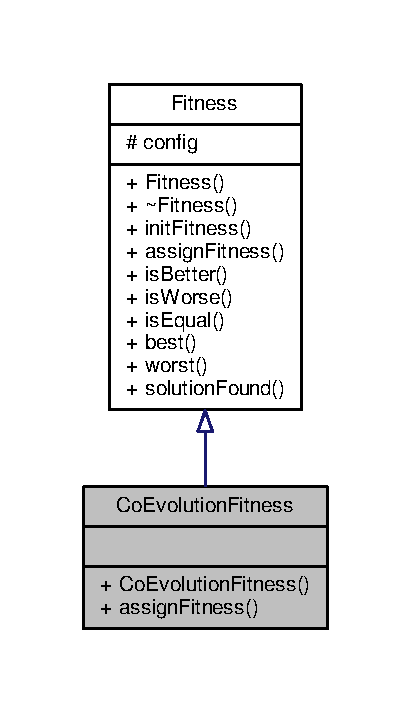
\includegraphics[width=197pt]{classCoEvolutionFitness__inherit__graph}
\end{center}
\end{figure}


Collaboration diagram for Co\+Evolution\+Fitness\+:
\nopagebreak
\begin{figure}[H]
\begin{center}
\leavevmode
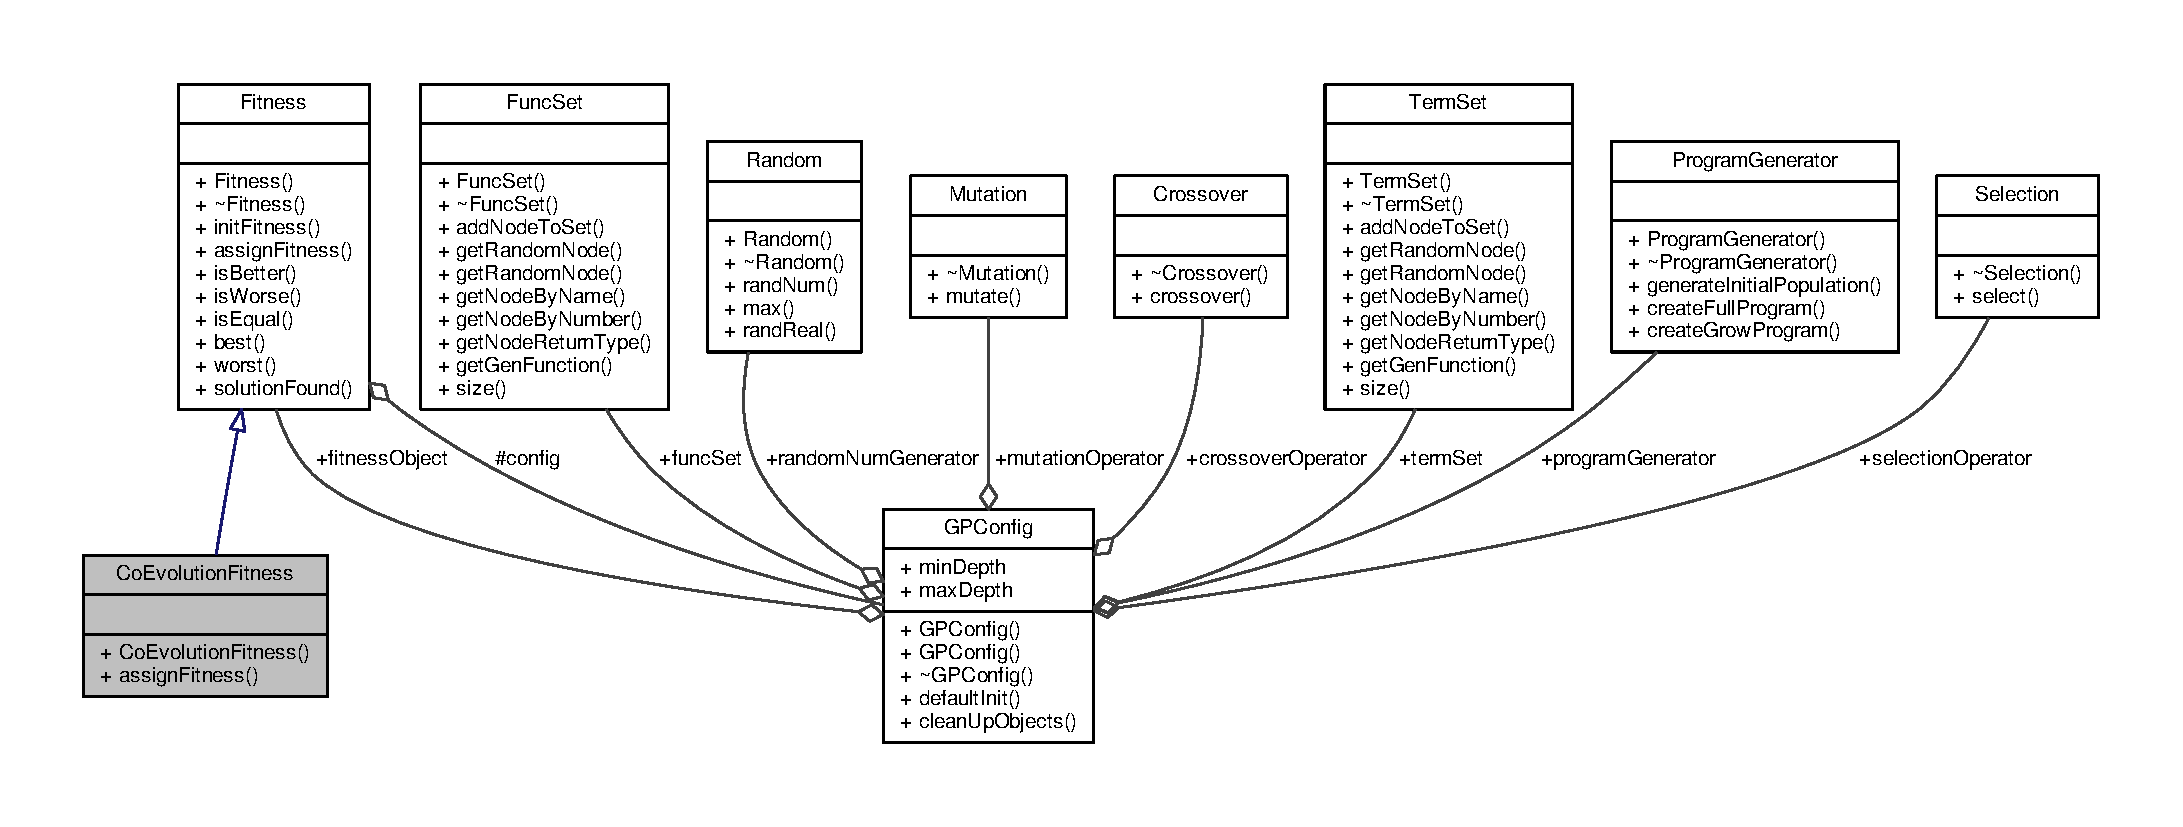
\includegraphics[width=350pt]{classCoEvolutionFitness__coll__graph}
\end{center}
\end{figure}
\subsection*{Public Member Functions}
\begin{DoxyCompactItemize}
\item 
\hypertarget{classCoEvolutionFitness_a555a6571bc8d63f197904135e56ac8db}{}\label{classCoEvolutionFitness_a555a6571bc8d63f197904135e56ac8db} 
{\bfseries Co\+Evolution\+Fitness} (\hyperlink{classGPConfig}{G\+P\+Config} $\ast$conf)
\item 
\hypertarget{classCoEvolutionFitness_a37662009bec754e555bd536803d5204c}{}\label{classCoEvolutionFitness_a37662009bec754e555bd536803d5204c} 
virtual void {\bfseries assign\+Fitness} (\hyperlink{classGeneticProgram}{Genetic\+Program} $\ast$$\ast$pop1, \hyperlink{classGeneticProgram}{Genetic\+Program} $\ast$$\ast$pop2, int num\+Individuals1, int num\+Individuals2)=0
\end{DoxyCompactItemize}
\subsection*{Additional Inherited Members}


The documentation for this class was generated from the following files\+:\begin{DoxyCompactItemize}
\item 
/home/\+Lach/npr-\/v109/\+R\+M\+I\+T\+G\+P.\+1.\+5/Co\+Evolution\+Fitness.\+h\item 
/home/\+Lach/npr-\/v109/\+R\+M\+I\+T\+G\+P.\+1.\+5/Co\+Evolution\+Fitness.\+cpp\end{DoxyCompactItemize}

\hypertarget{classCoEvolutionPopulation}{}\section{Co\+Evolution\+Population Class Reference}
\label{classCoEvolutionPopulation}\index{Co\+Evolution\+Population@{Co\+Evolution\+Population}}


Inheritance diagram for Co\+Evolution\+Population\+:
\nopagebreak
\begin{figure}[H]
\begin{center}
\leavevmode
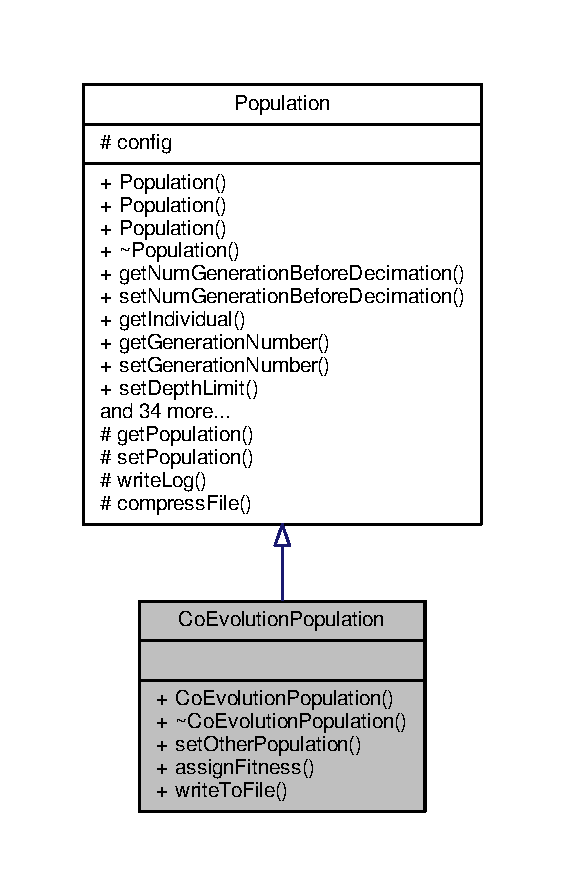
\includegraphics[width=271pt]{classCoEvolutionPopulation__inherit__graph}
\end{center}
\end{figure}


Collaboration diagram for Co\+Evolution\+Population\+:
\nopagebreak
\begin{figure}[H]
\begin{center}
\leavevmode
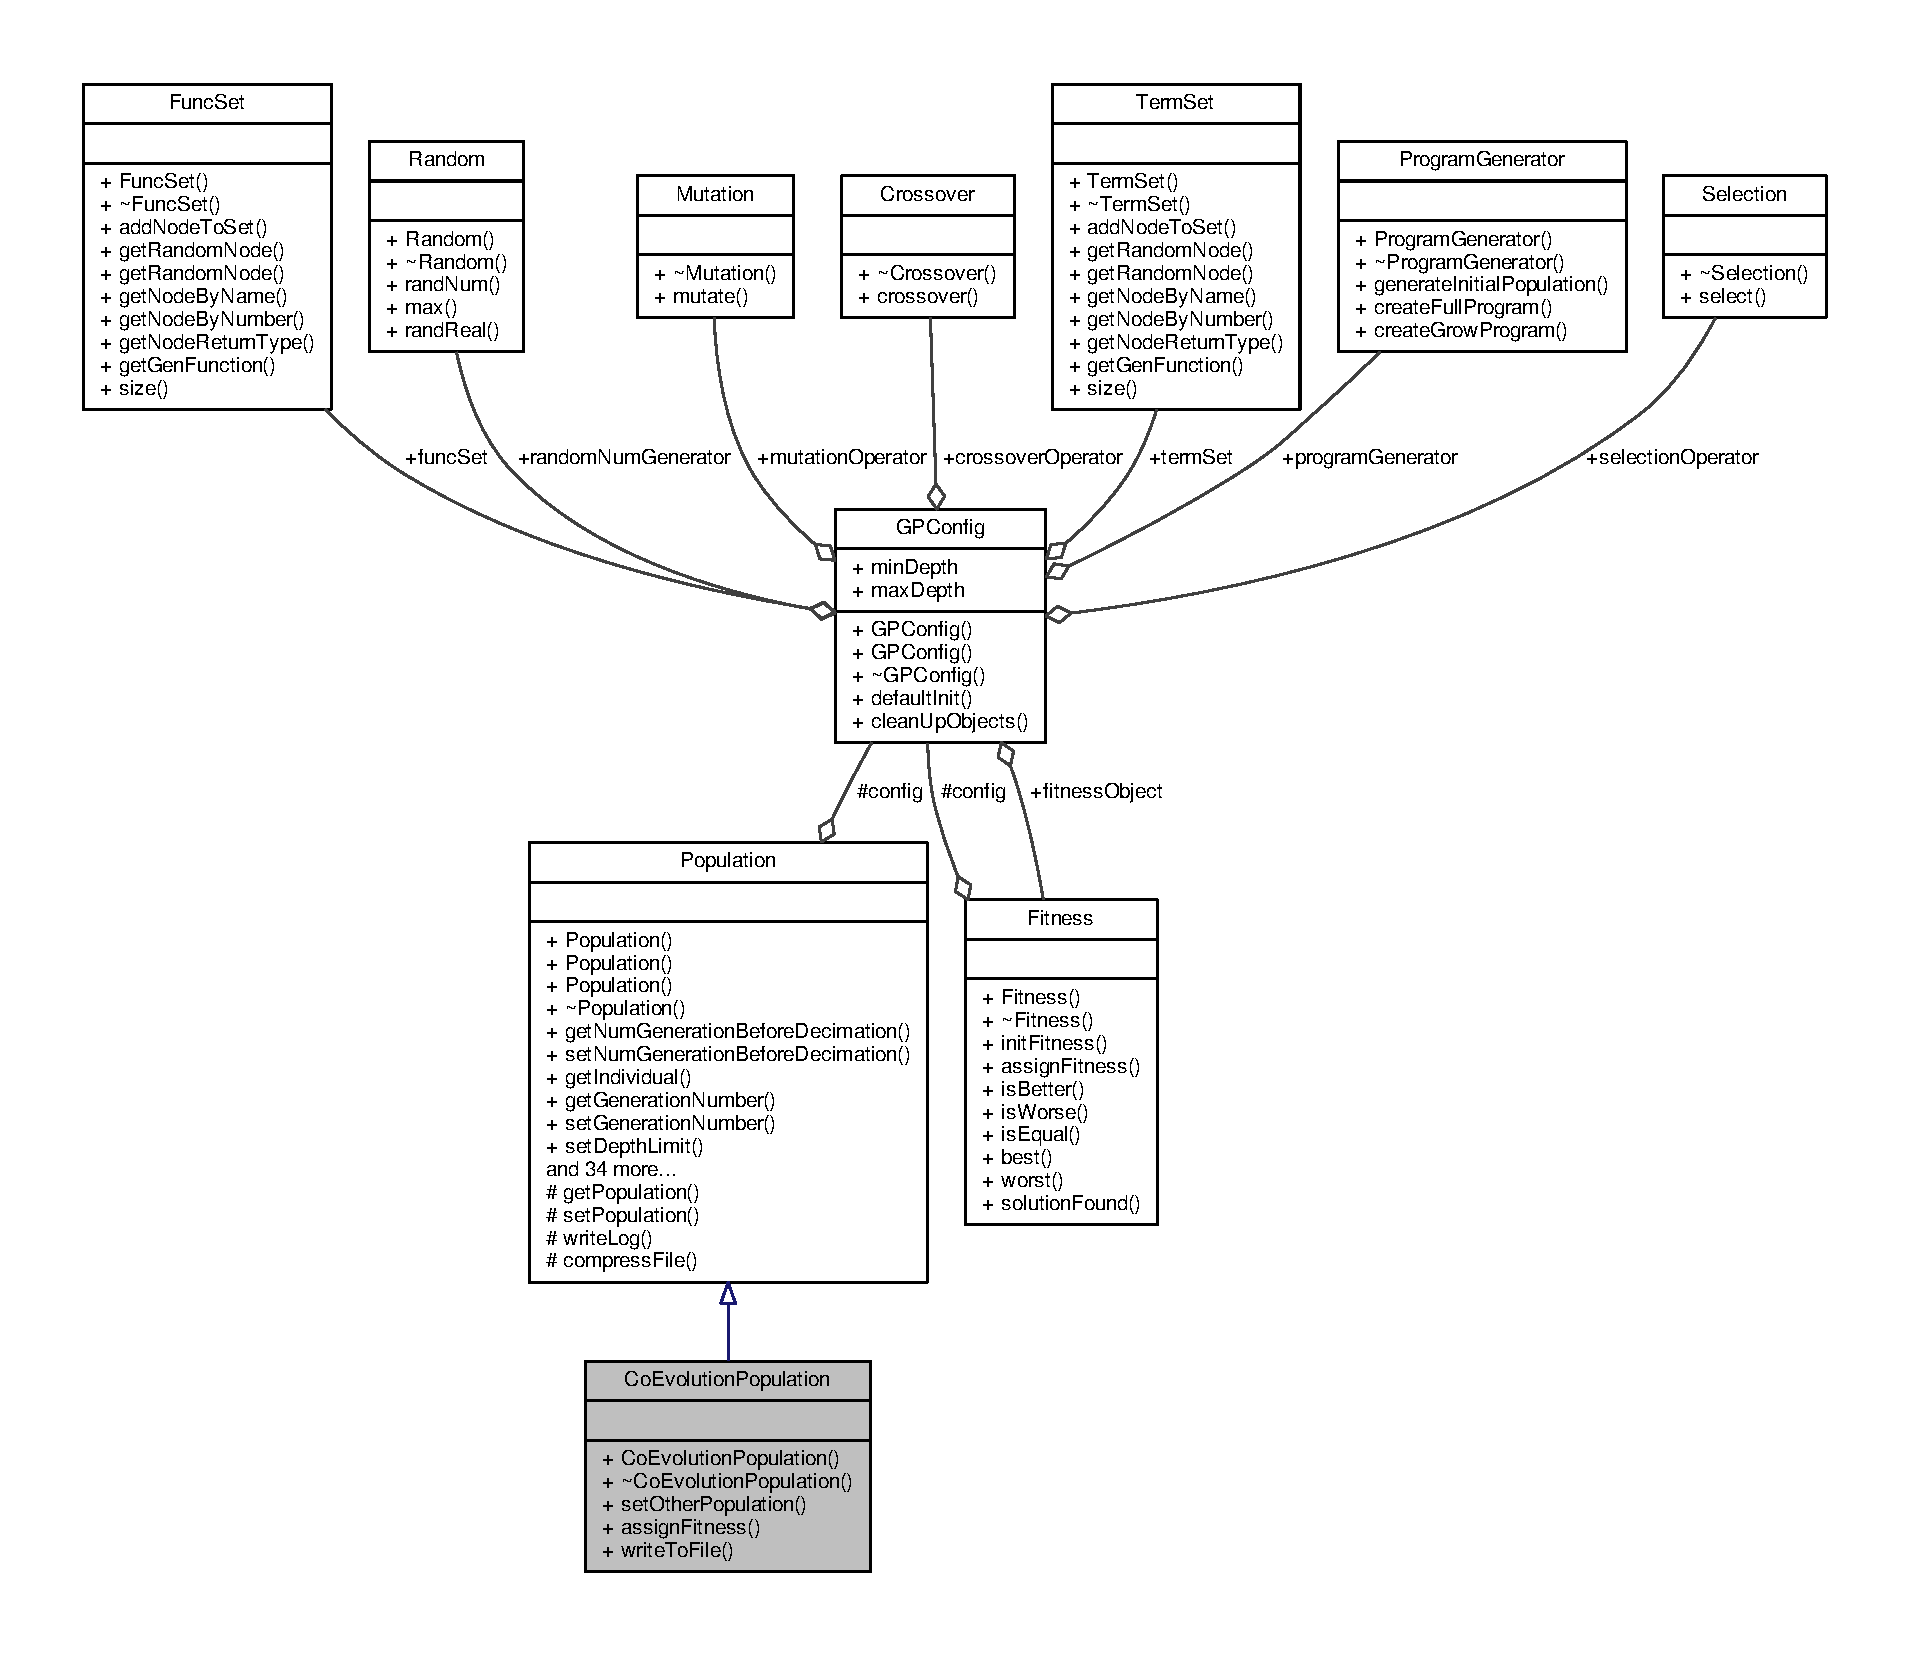
\includegraphics[width=350pt]{classCoEvolutionPopulation__coll__graph}
\end{center}
\end{figure}
\subsection*{Public Member Functions}
\begin{DoxyCompactItemize}
\item 
\hypertarget{classCoEvolutionPopulation_ae210feaa477d553c4bec4da4653cb863}{}\label{classCoEvolutionPopulation_ae210feaa477d553c4bec4da4653cb863} 
{\bfseries Co\+Evolution\+Population} (int size, char $\ast$log\+File\+Name, \hyperlink{classGPConfig}{G\+P\+Config} $\ast$conf, string pop\+Name)
\item 
\hypertarget{classCoEvolutionPopulation_a1b97173c538bca3a81a2617390dbe945}{}\label{classCoEvolutionPopulation_a1b97173c538bca3a81a2617390dbe945} 
void {\bfseries set\+Other\+Population} (\hyperlink{classCoEvolutionPopulation}{Co\+Evolution\+Population} $\ast$a\+Pop)
\item 
\hypertarget{classCoEvolutionPopulation_a40438230270750a7b0176e15845783ff}{}\label{classCoEvolutionPopulation_a40438230270750a7b0176e15845783ff} 
virtual void {\bfseries assign\+Fitness} ()
\item 
\hypertarget{classCoEvolutionPopulation_a827497c1c069d5d3cb4ad1aa8674a20a}{}\label{classCoEvolutionPopulation_a827497c1c069d5d3cb4ad1aa8674a20a} 
virtual void {\bfseries write\+To\+File} ()
\end{DoxyCompactItemize}
\subsection*{Additional Inherited Members}


The documentation for this class was generated from the following files\+:\begin{DoxyCompactItemize}
\item 
/home/\+Lach/npr-\/v109/\+R\+M\+I\+T\+G\+P.\+1.\+5/Co\+Evolution\+Population.\+h\item 
/home/\+Lach/npr-\/v109/\+R\+M\+I\+T\+G\+P.\+1.\+5/Co\+Evolution\+Population.\+cpp\end{DoxyCompactItemize}

\hypertarget{classColorConverter}{}\section{Color\+Converter Class Reference}
\label{classColorConverter}\index{Color\+Converter@{Color\+Converter}}


Collaboration diagram for Color\+Converter\+:
\nopagebreak
\begin{figure}[H]
\begin{center}
\leavevmode
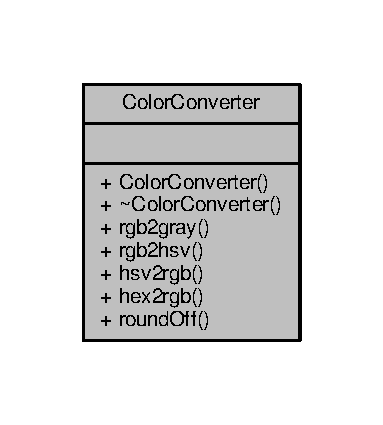
\includegraphics[width=184pt]{classColorConverter__coll__graph}
\end{center}
\end{figure}
\subsection*{Public Member Functions}
\begin{DoxyCompactItemize}
\item 
\hypertarget{classColorConverter_aa9abd3937e87e0fcb712d2ca7a611402}{}\label{classColorConverter_aa9abd3937e87e0fcb712d2ca7a611402} 
color\+\_\+t {\bfseries rgb2gray} (\hyperlink{structRGB}{R\+GB})
\item 
\hypertarget{classColorConverter_a351341558ba62951aefd6d3d9bf09785}{}\label{classColorConverter_a351341558ba62951aefd6d3d9bf09785} 
\hyperlink{structHSV}{H\+SV} {\bfseries rgb2hsv} (\hyperlink{structRGB}{R\+GB})
\item 
\hypertarget{classColorConverter_aca4539e968906df8d1ecd102464a0372}{}\label{classColorConverter_aca4539e968906df8d1ecd102464a0372} 
\hyperlink{structRGB}{R\+GB} {\bfseries hsv2rgb} (\hyperlink{structHSV}{H\+SV})
\item 
\hypertarget{classColorConverter_a43a52a206fb9f246d31af8f7e39b4110}{}\label{classColorConverter_a43a52a206fb9f246d31af8f7e39b4110} 
\hyperlink{structRGB}{R\+GB} {\bfseries hex2rgb} (std\+::string)
\item 
\hypertarget{classColorConverter_adb9a22672900e507c63b172a14713e95}{}\label{classColorConverter_adb9a22672900e507c63b172a14713e95} 
int {\bfseries round\+Off} (float, int)
\end{DoxyCompactItemize}


The documentation for this class was generated from the following files\+:\begin{DoxyCompactItemize}
\item 
/home/\+Lach/npr-\/v109/src\+\_\+109/Color\+Converter.\+h\item 
/home/\+Lach/npr-\/v109/src\+\_\+109/Color\+Converter.\+cpp\end{DoxyCompactItemize}

\hypertarget{classConfigReader}{}\section{Config\+Reader Class Reference}
\label{classConfigReader}\index{Config\+Reader@{Config\+Reader}}


Collaboration diagram for Config\+Reader\+:
\nopagebreak
\begin{figure}[H]
\begin{center}
\leavevmode
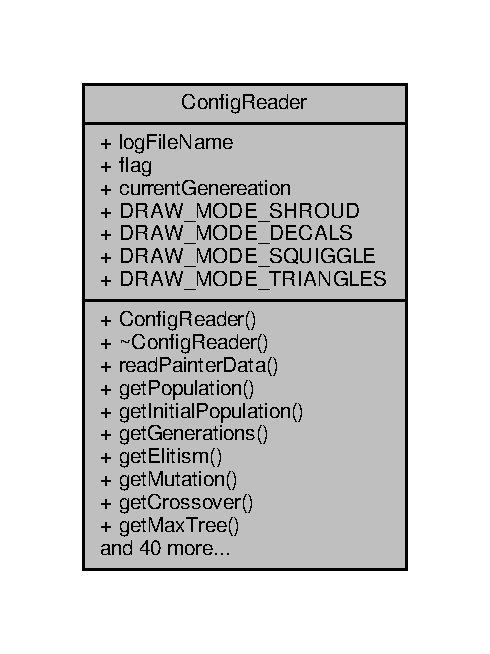
\includegraphics[width=235pt]{classConfigReader__coll__graph}
\end{center}
\end{figure}
\subsection*{Public Member Functions}
\begin{DoxyCompactItemize}
\item 
\hypertarget{classConfigReader_a0e567ddb371432f0c6bd5fa472304970}{}\label{classConfigReader_a0e567ddb371432f0c6bd5fa472304970} 
void {\bfseries read\+Painter\+Data} (const char $\ast$painter)
\item 
\hypertarget{classConfigReader_ad2c2a7bfc19b76357dc91d9def4c7992}{}\label{classConfigReader_ad2c2a7bfc19b76357dc91d9def4c7992} 
int {\bfseries get\+Population} ()
\item 
\hypertarget{classConfigReader_a5c2411ee0c0677015b9655dc7360c97e}{}\label{classConfigReader_a5c2411ee0c0677015b9655dc7360c97e} 
int {\bfseries get\+Initial\+Population} ()
\item 
\hypertarget{classConfigReader_a50cb73d4e053df9a16c16a6a650da147}{}\label{classConfigReader_a50cb73d4e053df9a16c16a6a650da147} 
int {\bfseries get\+Generations} ()
\item 
\hypertarget{classConfigReader_aaf6399eb399499490eae48fe29fe99eb}{}\label{classConfigReader_aaf6399eb399499490eae48fe29fe99eb} 
int {\bfseries get\+Elitism} ()
\item 
\hypertarget{classConfigReader_a9bb987d15fa1f2d13f7ada58e03e0a43}{}\label{classConfigReader_a9bb987d15fa1f2d13f7ada58e03e0a43} 
int {\bfseries get\+Mutation} ()
\item 
\hypertarget{classConfigReader_a1e2ade167d3e28489b4e2dc37242b8fd}{}\label{classConfigReader_a1e2ade167d3e28489b4e2dc37242b8fd} 
int {\bfseries get\+Crossover} ()
\item 
\hypertarget{classConfigReader_ae707de59f1e1c32bfa8f4961247758f6}{}\label{classConfigReader_ae707de59f1e1c32bfa8f4961247758f6} 
int {\bfseries get\+Max\+Tree} ()
\item 
\hypertarget{classConfigReader_ac8b0ed0d215cfbdb595f9ca91db0bc5c}{}\label{classConfigReader_ac8b0ed0d215cfbdb595f9ca91db0bc5c} 
int {\bfseries get\+Min\+Tree} ()
\item 
\hypertarget{classConfigReader_a48f25599934dd6a80694e312139d7fa8}{}\label{classConfigReader_a48f25599934dd6a80694e312139d7fa8} 
bool {\bfseries get\+Fuzzy\+Edges} ()
\item 
\hypertarget{classConfigReader_abc7d4bab01a5e1eeabb30e185a230455}{}\label{classConfigReader_abc7d4bab01a5e1eeabb30e185a230455} 
int {\bfseries get\+Sat\+Canny\+Lo} ()
\item 
\hypertarget{classConfigReader_ad275c15d54c720a54cd4010b5dc6a193}{}\label{classConfigReader_ad275c15d54c720a54cd4010b5dc6a193} 
int {\bfseries get\+Sat\+Canny\+Hi} ()
\item 
\hypertarget{classConfigReader_aecef166e19340044e96cc9aa033c2b0b}{}\label{classConfigReader_aecef166e19340044e96cc9aa033c2b0b} 
int {\bfseries get\+Val\+Canny\+Lo} ()
\item 
\hypertarget{classConfigReader_a5cc8adc5919047dfc7794a1ade63d031}{}\label{classConfigReader_a5cc8adc5919047dfc7794a1ade63d031} 
int {\bfseries get\+Val\+Canny\+Hi} ()
\item 
\hypertarget{classConfigReader_a825c0cdf7ac8c8698982d45730c656c8}{}\label{classConfigReader_a825c0cdf7ac8c8698982d45730c656c8} 
float {\bfseries get\+Fitness\+Target} ()
\item 
\hypertarget{classConfigReader_a3f399e2dc3622639d9fecff36e9951d2}{}\label{classConfigReader_a3f399e2dc3622639d9fecff36e9951d2} 
int {\bfseries get\+Random\+Seed} ()
\item 
\hypertarget{classConfigReader_ab7c21d8d74d01907e4ef64f2033bcaba}{}\label{classConfigReader_ab7c21d8d74d01907e4ef64f2033bcaba} 
int {\bfseries get\+Canvas\+BG} ()
\item 
\hypertarget{classConfigReader_af10edf0066b89aeb465f80b869c6b1e3}{}\label{classConfigReader_af10edf0066b89aeb465f80b869c6b1e3} 
int {\bfseries get\+Canvas\+B\+G\+\_\+\+Red} ()
\item 
\hypertarget{classConfigReader_a206a96e4b64d12105e36ef9ad98bf4ff}{}\label{classConfigReader_a206a96e4b64d12105e36ef9ad98bf4ff} 
int {\bfseries get\+Canvas\+B\+G\+\_\+\+Green} ()
\item 
\hypertarget{classConfigReader_a61718c31162418d22f3119bfc9d43f75}{}\label{classConfigReader_a61718c31162418d22f3119bfc9d43f75} 
int {\bfseries get\+Canvas\+B\+G\+\_\+\+Blue} ()
\item 
\hypertarget{classConfigReader_aa0093d6cc78780960771c5abd12937a1}{}\label{classConfigReader_aa0093d6cc78780960771c5abd12937a1} 
int {\bfseries get\+Colour\+Updater} ()
\item 
\hypertarget{classConfigReader_ae408fab7b0a2a214621f02d0c019a4e7}{}\label{classConfigReader_ae408fab7b0a2a214621f02d0c019a4e7} 
int {\bfseries get\+Colour\+Mode} ()
\item 
\hypertarget{classConfigReader_af337f0c19e0ed70d586a7471fc0b2d5e}{}\label{classConfigReader_af337f0c19e0ed70d586a7471fc0b2d5e} 
int {\bfseries get\+First\+Line\+Length} ()
\item 
\hypertarget{classConfigReader_a5f2b66c0fecfb1c542c68c3f89d4361f}{}\label{classConfigReader_a5f2b66c0fecfb1c542c68c3f89d4361f} 
int {\bfseries get\+Second\+Line\+Length} ()
\item 
\hypertarget{classConfigReader_a09ef925e405ebd002bbe61c554020dcc}{}\label{classConfigReader_a09ef925e405ebd002bbe61c554020dcc} 
int {\bfseries get\+Type\+Triangle} ()
\item 
\hypertarget{classConfigReader_a8f9d90b2ea2da85939040a41b1395260}{}\label{classConfigReader_a8f9d90b2ea2da85939040a41b1395260} 
std\+::string {\bfseries get\+Custom\+Decal\+File\+Name} ()
\item 
\hypertarget{classConfigReader_a6f42945c6aa5a1669ccd59c3f998b456}{}\label{classConfigReader_a6f42945c6aa5a1669ccd59c3f998b456} 
std\+::string {\bfseries get\+Path\+To\+Target} ()
\item 
\hypertarget{classConfigReader_a44d2bef5c4bc3d42ff4d5e1a6d6dae4f}{}\label{classConfigReader_a44d2bef5c4bc3d42ff4d5e1a6d6dae4f} 
std\+::string {\bfseries get\+Path\+To\+Mask} ()
\item 
\hypertarget{classConfigReader_a9fe59626354c78f6e52f06ff98de38c6}{}\label{classConfigReader_a9fe59626354c78f6e52f06ff98de38c6} 
std\+::string {\bfseries get\+Path\+To\+Output} ()
\item 
\hypertarget{classConfigReader_a90abd02c164c974d5c67577ee29c1c54}{}\label{classConfigReader_a90abd02c164c974d5c67577ee29c1c54} 
std\+::string {\bfseries get\+Path\+To\+Palette} ()
\item 
\hypertarget{classConfigReader_acc7926f146161c7512631296c6169c27}{}\label{classConfigReader_acc7926f146161c7512631296c6169c27} 
std\+::string {\bfseries get\+Target\+File\+Name} ()
\item 
\hypertarget{classConfigReader_ac130d7d879988452891fc1f4d5e89b1a}{}\label{classConfigReader_ac130d7d879988452891fc1f4d5e89b1a} 
std\+::string {\bfseries get\+Palette} ()
\item 
\hypertarget{classConfigReader_a80d01e04ca22ca126bbdbc476984cfea}{}\label{classConfigReader_a80d01e04ca22ca126bbdbc476984cfea} 
std\+::string {\bfseries get\+Version} ()
\item 
\hypertarget{classConfigReader_a5a2e68a5fb89b5d0bb2b8d38150edcd1}{}\label{classConfigReader_a5a2e68a5fb89b5d0bb2b8d38150edcd1} 
bool {\bfseries get\+Line\+Art\+Thickness} ()
\item 
\hypertarget{classConfigReader_ab4f64f1b863a6d78ef8087d1d41c6889}{}\label{classConfigReader_ab4f64f1b863a6d78ef8087d1d41c6889} 
int {\bfseries get\+Draw\+Mode} ()
\item 
\hypertarget{classConfigReader_a813f80a6afee19bdfd1787db5c277676}{}\label{classConfigReader_a813f80a6afee19bdfd1787db5c277676} 
double {\bfseries get\+Fitness\+Render\+Threshold} ()
\item 
\hypertarget{classConfigReader_abe4991a967a948f5bfa7d61eca9e26c2}{}\label{classConfigReader_abe4991a967a948f5bfa7d61eca9e26c2} 
bool {\bfseries get\+Prog2} ()
\item 
\hypertarget{classConfigReader_a15c4ba819559d15420c43c40b455972a}{}\label{classConfigReader_a15c4ba819559d15420c43c40b455972a} 
bool {\bfseries get\+Prog3} ()
\item 
\hypertarget{classConfigReader_a73b004a202d836b0f5947675529dbb4c}{}\label{classConfigReader_a73b004a202d836b0f5947675529dbb4c} 
bool {\bfseries get\+Prog4} ()
\item 
\hypertarget{classConfigReader_ac33a1ec754771eb38d945e312493fc70}{}\label{classConfigReader_ac33a1ec754771eb38d945e312493fc70} 
bool {\bfseries get\+Using\+Adaptive\+Canvas} ()
\item 
\hypertarget{classConfigReader_ad2722e1f259e6a4e46b5dc0166fdf80d}{}\label{classConfigReader_ad2722e1f259e6a4e46b5dc0166fdf80d} 
bool {\bfseries get\+Fast\+Shroud} ()
\item 
\hypertarget{classConfigReader_a16ec9fa2175b2c7f28253ca3ec05c2da}{}\label{classConfigReader_a16ec9fa2175b2c7f28253ca3ec05c2da} 
int {\bfseries get\+Line\+Art\+Color\+Mode} ()
\item 
\hypertarget{classConfigReader_a8b50213030f7964d77e8989f8ee6c5e4}{}\label{classConfigReader_a8b50213030f7964d77e8989f8ee6c5e4} 
int {\bfseries get\+Shroud\+Pixel\+Strategy} ()
\item 
\hypertarget{classConfigReader_ac48c38cb4fd2d04c7761b4813d94cd90}{}\label{classConfigReader_ac48c38cb4fd2d04c7761b4813d94cd90} 
int {\bfseries get\+Tournament\+Size} ()
\item 
\hypertarget{classConfigReader_aaf1d7c03b3b4b3e71e12e6161b09db34}{}\label{classConfigReader_aaf1d7c03b3b4b3e71e12e6161b09db34} 
void {\bfseries set\+Shroud\+Log\+Name} (char $\ast$newlog\+File\+Name)
\item 
\hypertarget{classConfigReader_ac5df2afab92273c5a69c61fb8ffc9355}{}\label{classConfigReader_ac5df2afab92273c5a69c61fb8ffc9355} 
char $\ast$ {\bfseries get\+Shroud\+Log\+Name} ()
\item 
\hypertarget{classConfigReader_a7bf5f509fd6103cf351c384ddde32149}{}\label{classConfigReader_a7bf5f509fd6103cf351c384ddde32149} 
void {\bfseries set\+Error\+Log\+Bad} (bool newflag)
\item 
\hypertarget{classConfigReader_a5b5baa8c5865fd75f87d3fe69dc2f814}{}\label{classConfigReader_a5b5baa8c5865fd75f87d3fe69dc2f814} 
string {\bfseries get\+Error\+Log\+Bad} ()
\end{DoxyCompactItemize}
\subsection*{Public Attributes}
\begin{DoxyCompactItemize}
\item 
\hypertarget{classConfigReader_adff3f922c1af68d2ff3ffb2935f9ff7b}{}\label{classConfigReader_adff3f922c1af68d2ff3ffb2935f9ff7b} 
char $\ast$ {\bfseries log\+File\+Name}
\item 
\hypertarget{classConfigReader_abab3606d626f5ae659ffd34a6ecab8c2}{}\label{classConfigReader_abab3606d626f5ae659ffd34a6ecab8c2} 
bool {\bfseries flag}
\item 
\hypertarget{classConfigReader_a1ab9194bdcf3d05cddc5ddcfe99dc08f}{}\label{classConfigReader_a1ab9194bdcf3d05cddc5ddcfe99dc08f} 
int {\bfseries current\+Genereation}
\end{DoxyCompactItemize}
\subsection*{Static Public Attributes}
\begin{DoxyCompactItemize}
\item 
\hypertarget{classConfigReader_a728af86620d2f7bd22f8f50dc576dfbc}{}\label{classConfigReader_a728af86620d2f7bd22f8f50dc576dfbc} 
static const int {\bfseries D\+R\+A\+W\+\_\+\+M\+O\+D\+E\+\_\+\+S\+H\+R\+O\+UD} = 0
\item 
\hypertarget{classConfigReader_af7fb8fa1f2cc76913afc78a2726e44a6}{}\label{classConfigReader_af7fb8fa1f2cc76913afc78a2726e44a6} 
static const int {\bfseries D\+R\+A\+W\+\_\+\+M\+O\+D\+E\+\_\+\+D\+E\+C\+A\+LS} = 1
\item 
\hypertarget{classConfigReader_a51777b70066b67ddb71b1f2a0762e20a}{}\label{classConfigReader_a51777b70066b67ddb71b1f2a0762e20a} 
static const int {\bfseries D\+R\+A\+W\+\_\+\+M\+O\+D\+E\+\_\+\+S\+Q\+U\+I\+G\+G\+LE} = 2
\item 
\hypertarget{classConfigReader_aeb8151f583f4f6b01c7c404dec49a74c}{}\label{classConfigReader_aeb8151f583f4f6b01c7c404dec49a74c} 
static const int {\bfseries D\+R\+A\+W\+\_\+\+M\+O\+D\+E\+\_\+\+T\+R\+I\+A\+N\+G\+L\+ES} = 3
\end{DoxyCompactItemize}


The documentation for this class was generated from the following files\+:\begin{DoxyCompactItemize}
\item 
/home/\+Lach/npr-\/v109/src\+\_\+109/Config\+Reader.\+h\item 
/home/\+Lach/npr-\/v109/src\+\_\+109/Config\+Reader.\+cpp\end{DoxyCompactItemize}

\hypertarget{structCoord}{}\section{Coord Struct Reference}
\label{structCoord}\index{Coord@{Coord}}


Collaboration diagram for Coord\+:
\nopagebreak
\begin{figure}[H]
\begin{center}
\leavevmode
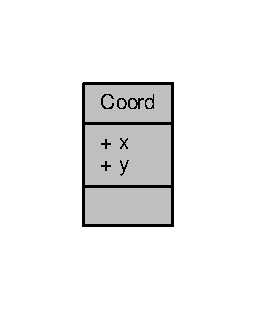
\includegraphics[width=123pt]{structCoord__coll__graph}
\end{center}
\end{figure}
\subsection*{Public Attributes}
\begin{DoxyCompactItemize}
\item 
\hypertarget{structCoord_a089b098faaca481f53834c7cd7605da5}{}\label{structCoord_a089b098faaca481f53834c7cd7605da5} 
float {\bfseries x}
\item 
\hypertarget{structCoord_a55a67a26b632758699c9f999348d9f06}{}\label{structCoord_a55a67a26b632758699c9f999348d9f06} 
float {\bfseries y}
\end{DoxyCompactItemize}


The documentation for this struct was generated from the following file\+:\begin{DoxyCompactItemize}
\item 
/home/\+Lach/npr-\/v109/src\+\_\+109/Utility.\+h\end{DoxyCompactItemize}

\hypertarget{classCrossover}{}\section{Crossover Class Reference}
\label{classCrossover}\index{Crossover@{Crossover}}


Collaboration diagram for Crossover\+:
\nopagebreak
\begin{figure}[H]
\begin{center}
\leavevmode
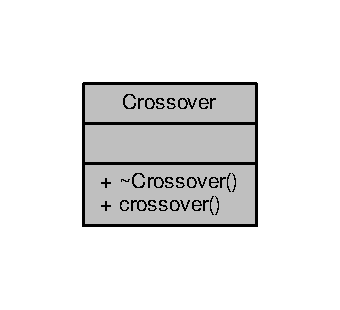
\includegraphics[width=163pt]{classCrossover__coll__graph}
\end{center}
\end{figure}
\subsection*{Public Member Functions}
\begin{DoxyCompactItemize}
\item 
\hypertarget{classCrossover_a52fadaa841c3fc0113b991da70b3675f}{}\label{classCrossover_a52fadaa841c3fc0113b991da70b3675f} 
virtual void {\bfseries crossover} (\hyperlink{classGeneticProgram}{Genetic\+Program} \&gp1, \hyperlink{classGeneticProgram}{Genetic\+Program} \&gp2, int num\+Retries, \hyperlink{classGPConfig}{G\+P\+Config} $\ast$config)
\end{DoxyCompactItemize}


The documentation for this class was generated from the following files\+:\begin{DoxyCompactItemize}
\item 
/home/\+Lach/npr-\/v109/\+R\+M\+I\+T\+G\+P.\+1.\+5/Crossover.\+h\item 
/home/\+Lach/npr-\/v109/\+R\+M\+I\+T\+G\+P.\+1.\+5/Crossover.\+cpp\end{DoxyCompactItemize}

\hypertarget{classDecal}{}\section{Decal Class Reference}
\label{classDecal}\index{Decal@{Decal}}


Collaboration diagram for Decal\+:
\nopagebreak
\begin{figure}[H]
\begin{center}
\leavevmode
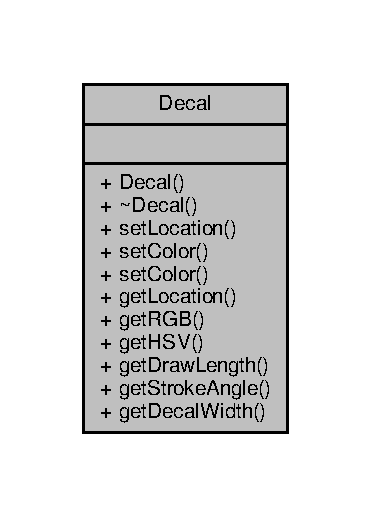
\includegraphics[width=178pt]{classDecal__coll__graph}
\end{center}
\end{figure}
\subsection*{Public Member Functions}
\begin{DoxyCompactItemize}
\item 
\hypertarget{classDecal_a101d637231bbe15438573ff44481e025}{}\label{classDecal_a101d637231bbe15438573ff44481e025} 
{\bfseries Decal} (\hyperlink{classConfigReader}{Config\+Reader} $\ast$reader, int min\+Dim, int max\+Dim)
\item 
\hypertarget{classDecal_aca34cd0f099e08c77d5309eb1177b6db}{}\label{classDecal_aca34cd0f099e08c77d5309eb1177b6db} 
void {\bfseries set\+Location} (float f1, float f2)
\item 
\hypertarget{classDecal_ad59c6e4cfb8b06e7403aaf7a12a96ba8}{}\label{classDecal_ad59c6e4cfb8b06e7403aaf7a12a96ba8} 
void {\bfseries set\+Color} (float f1, float f2, float f3)
\item 
\hypertarget{classDecal_a4b3153696a223ec85c53e22876023a14}{}\label{classDecal_a4b3153696a223ec85c53e22876023a14} 
void {\bfseries set\+Color} (\hyperlink{structHSV}{H\+SV} col)
\item 
\hypertarget{classDecal_abcf93a8a28597b3e07ca8268af2ef049}{}\label{classDecal_abcf93a8a28597b3e07ca8268af2ef049} 
\hyperlink{structCoord}{Coord} {\bfseries get\+Location} ()
\item 
\hypertarget{classDecal_a88024aec965f854e6ee74867b107963c}{}\label{classDecal_a88024aec965f854e6ee74867b107963c} 
\hyperlink{structRGB}{R\+GB} {\bfseries get\+R\+GB} ()
\item 
\hypertarget{classDecal_a78513a5e1b703ae65933f20f45cf8011}{}\label{classDecal_a78513a5e1b703ae65933f20f45cf8011} 
\hyperlink{structHSV}{H\+SV} {\bfseries get\+H\+SV} ()
\item 
\hypertarget{classDecal_a7d789f497a9019c4ab1fc2377038fc32}{}\label{classDecal_a7d789f497a9019c4ab1fc2377038fc32} 
int {\bfseries get\+Draw\+Length} ()
\item 
\hypertarget{classDecal_ad25e74f9b24b4487713a64fd2b8711c0}{}\label{classDecal_ad25e74f9b24b4487713a64fd2b8711c0} 
double {\bfseries get\+Stroke\+Angle} ()
\item 
\hypertarget{classDecal_ab455f1768097265f73022194f2830861}{}\label{classDecal_ab455f1768097265f73022194f2830861} 
int {\bfseries get\+Decal\+Width} ()
\end{DoxyCompactItemize}


The documentation for this class was generated from the following files\+:\begin{DoxyCompactItemize}
\item 
/home/\+Lach/npr-\/v109/src\+\_\+109/Decal.\+h\item 
/home/\+Lach/npr-\/v109/src\+\_\+109/Decal.\+cpp\end{DoxyCompactItemize}

\hypertarget{classDecalCanvas}{}\section{Decal\+Canvas Class Reference}
\label{classDecalCanvas}\index{Decal\+Canvas@{Decal\+Canvas}}


Inheritance diagram for Decal\+Canvas\+:
\nopagebreak
\begin{figure}[H]
\begin{center}
\leavevmode
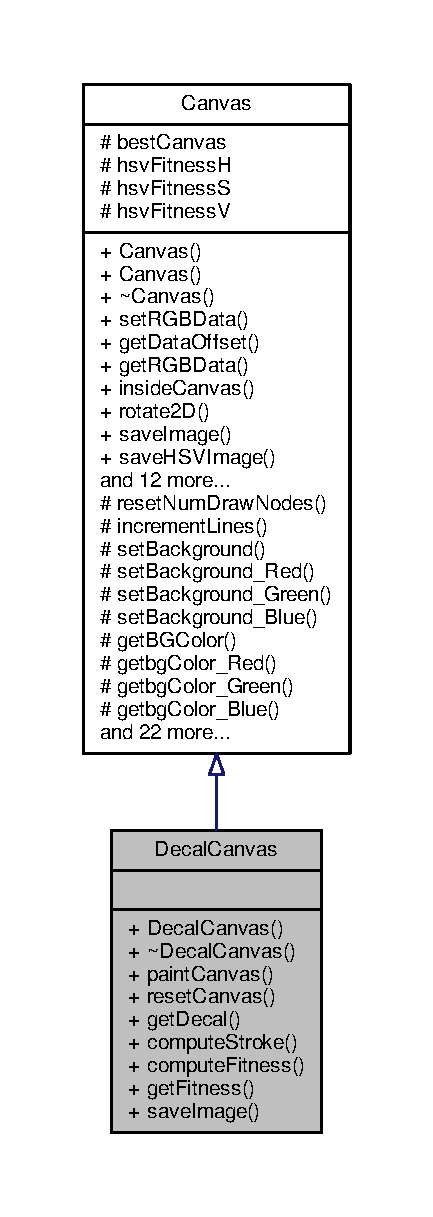
\includegraphics[height=550pt]{classDecalCanvas__inherit__graph}
\end{center}
\end{figure}


Collaboration diagram for Decal\+Canvas\+:
\nopagebreak
\begin{figure}[H]
\begin{center}
\leavevmode
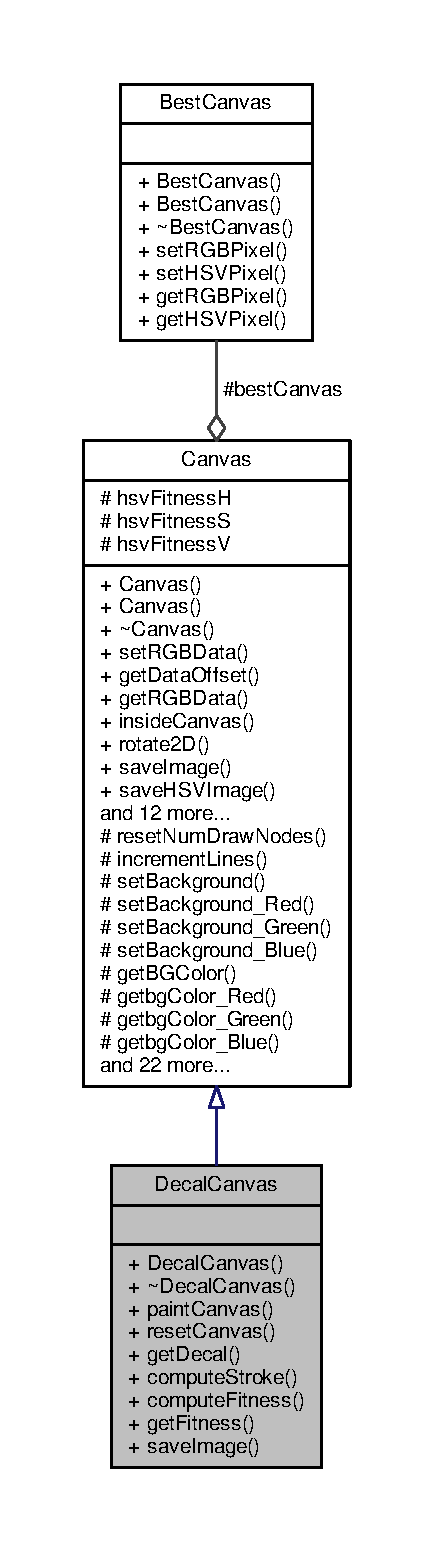
\includegraphics[height=550pt]{classDecalCanvas__coll__graph}
\end{center}
\end{figure}
\subsection*{Public Member Functions}
\begin{DoxyCompactItemize}
\item 
\hypertarget{classDecalCanvas_ad00c8fbce88da1fd173f7da551f7ef95}{}\label{classDecalCanvas_ad00c8fbce88da1fd173f7da551f7ef95} 
{\bfseries Decal\+Canvas} (\hyperlink{classTarget}{Target} $\ast$t, color\+\_\+t bg, \hyperlink{classBestCanvas}{Best\+Canvas} $\ast$bc, \hyperlink{classConfigReader}{Config\+Reader} $\ast$reader)
\item 
\hypertarget{classDecalCanvas_adbf1ef248c1cf7b6ed09abfa1ec05c08}{}\label{classDecalCanvas_adbf1ef248c1cf7b6ed09abfa1ec05c08} 
void {\bfseries paint\+Canvas} (vector$<$ float $>$)
\item 
\hypertarget{classDecalCanvas_a64baadb9a31c5aa598a45ce402d6d66a}{}\label{classDecalCanvas_a64baadb9a31c5aa598a45ce402d6d66a} 
void {\bfseries reset\+Canvas} ()
\item 
\hypertarget{classDecalCanvas_a8f122bff9c7696f184b8903dbb295af5}{}\label{classDecalCanvas_a8f122bff9c7696f184b8903dbb295af5} 
\hyperlink{classDecal}{Decal} $\ast$ {\bfseries get\+Decal} ()
\item 
\hypertarget{classDecalCanvas_aa2d4c9185e12bad6aa590a9f58477063}{}\label{classDecalCanvas_aa2d4c9185e12bad6aa590a9f58477063} 
void {\bfseries compute\+Stroke} ()
\item 
\hypertarget{classDecalCanvas_a6f9a66f4a1f22e227ef9120410534531}{}\label{classDecalCanvas_a6f9a66f4a1f22e227ef9120410534531} 
void {\bfseries compute\+Fitness} ()
\item 
\hypertarget{classDecalCanvas_a1e0134f001a92ce161838286fa73ad69}{}\label{classDecalCanvas_a1e0134f001a92ce161838286fa73ad69} 
float {\bfseries get\+Fitness} ()
\item 
\hypertarget{classDecalCanvas_a7309b13ba847f9efd36f94f50d2238bd}{}\label{classDecalCanvas_a7309b13ba847f9efd36f94f50d2238bd} 
bool {\bfseries save\+Image} (char $\ast$filename)
\end{DoxyCompactItemize}
\subsection*{Additional Inherited Members}


The documentation for this class was generated from the following files\+:\begin{DoxyCompactItemize}
\item 
/home/\+Lach/npr-\/v109/src\+\_\+109/Decal\+Canvas.\+h\item 
/home/\+Lach/npr-\/v109/src\+\_\+109/Decal\+Canvas.\+cpp\end{DoxyCompactItemize}

\hypertarget{classDraw2}{}\section{Draw2 Class Reference}
\label{classDraw2}\index{Draw2@{Draw2}}


Inheritance diagram for Draw2\+:
\nopagebreak
\begin{figure}[H]
\begin{center}
\leavevmode
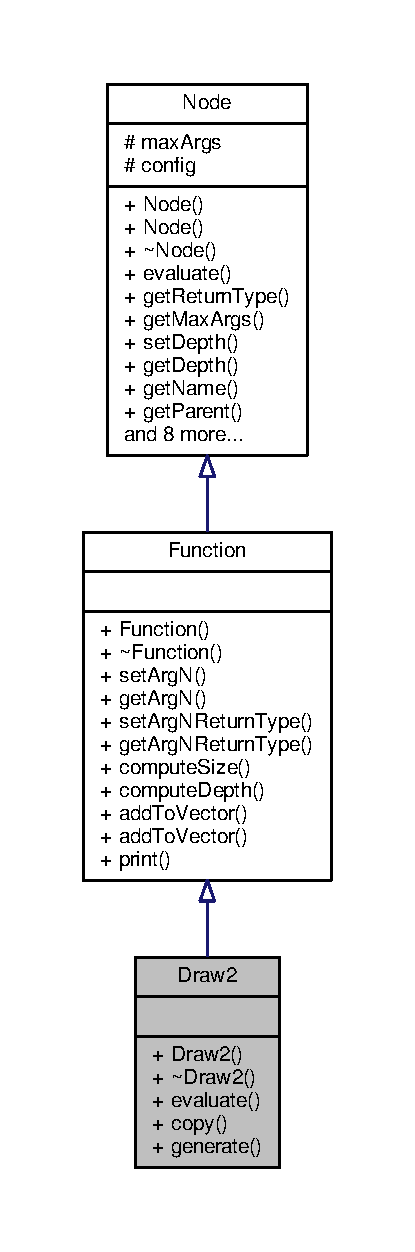
\includegraphics[height=550pt]{classDraw2__inherit__graph}
\end{center}
\end{figure}


Collaboration diagram for Draw2\+:
\nopagebreak
\begin{figure}[H]
\begin{center}
\leavevmode
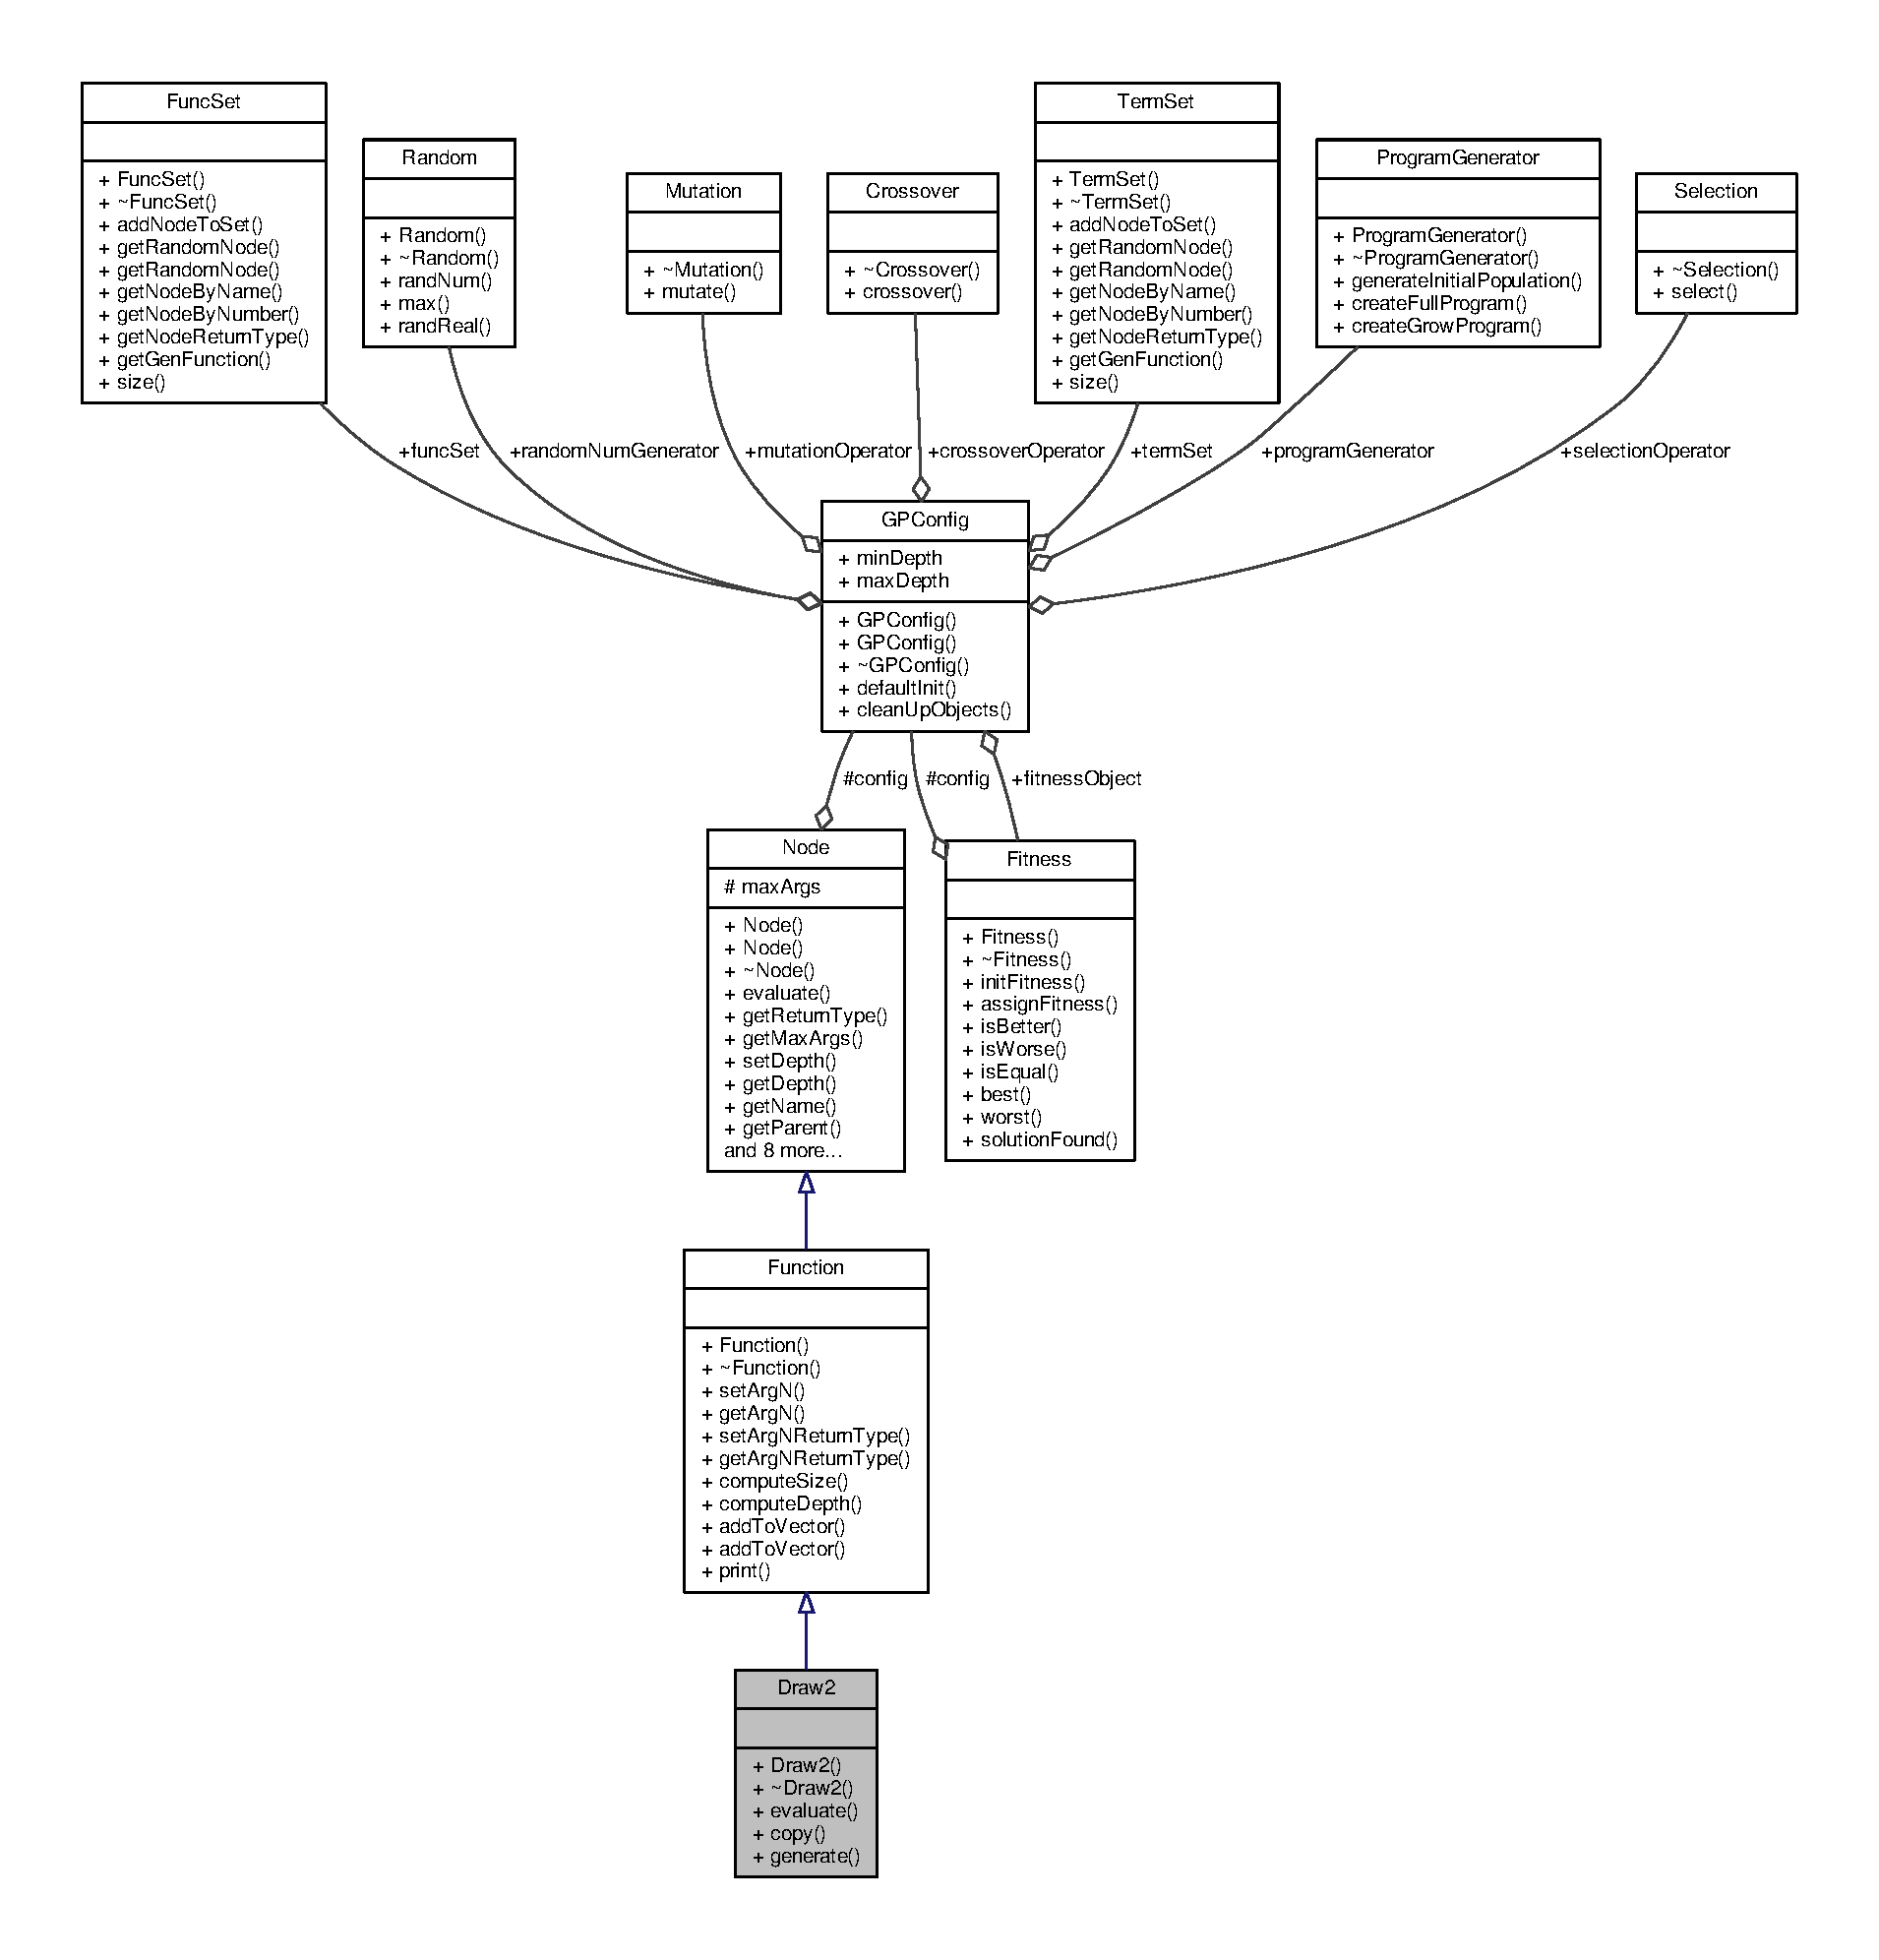
\includegraphics[width=350pt]{classDraw2__coll__graph}
\end{center}
\end{figure}
\subsection*{Public Member Functions}
\begin{DoxyCompactItemize}
\item 
\hypertarget{classDraw2_a60ad134856f332bd4e3134eb3b0cef48}{}\label{classDraw2_a60ad134856f332bd4e3134eb3b0cef48} 
{\bfseries Draw2} (\hyperlink{classGPConfig}{G\+P\+Config} $\ast$conf)
\item 
\hypertarget{classDraw2_affe1fb09b91b328b5f9edf6a8e44995b}{}\label{classDraw2_affe1fb09b91b328b5f9edf6a8e44995b} 
virtual void {\bfseries evaluate} (\hyperlink{classReturnData}{Return\+Data} $\ast$out)
\item 
\hypertarget{classDraw2_af82e7c3c4e46ad383ce3cb4a8589872d}{}\label{classDraw2_af82e7c3c4e46ad383ce3cb4a8589872d} 
virtual \hyperlink{classNode}{Node} $\ast$ {\bfseries copy} ()
\end{DoxyCompactItemize}
\subsection*{Static Public Member Functions}
\begin{DoxyCompactItemize}
\item 
\hypertarget{classDraw2_acc0991ece5e007a9cca5d3f84c4f5bb4}{}\label{classDraw2_acc0991ece5e007a9cca5d3f84c4f5bb4} 
static \hyperlink{classFunction}{Function} $\ast$ {\bfseries generate} (const string \&name, \hyperlink{classGPConfig}{G\+P\+Config} $\ast$conf)
\end{DoxyCompactItemize}
\subsection*{Additional Inherited Members}


The documentation for this class was generated from the following files\+:\begin{DoxyCompactItemize}
\item 
/home/\+Lach/npr-\/v109/src\+\_\+109/Draw2.\+h\item 
/home/\+Lach/npr-\/v109/src\+\_\+109/Draw2.\+cpp\end{DoxyCompactItemize}

\hypertarget{classDraw4}{}\section{Draw4 Class Reference}
\label{classDraw4}\index{Draw4@{Draw4}}


Inheritance diagram for Draw4\+:
\nopagebreak
\begin{figure}[H]
\begin{center}
\leavevmode
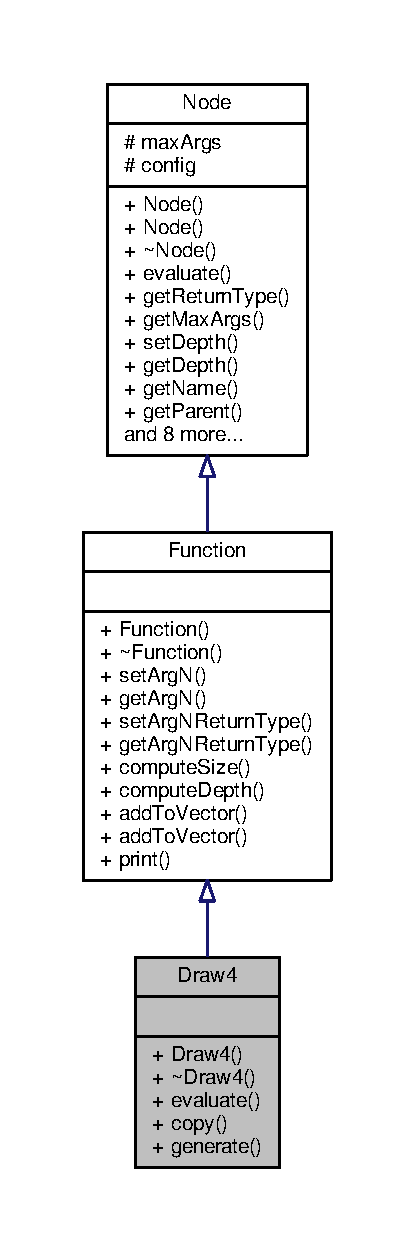
\includegraphics[height=550pt]{classDraw4__inherit__graph}
\end{center}
\end{figure}


Collaboration diagram for Draw4\+:
\nopagebreak
\begin{figure}[H]
\begin{center}
\leavevmode
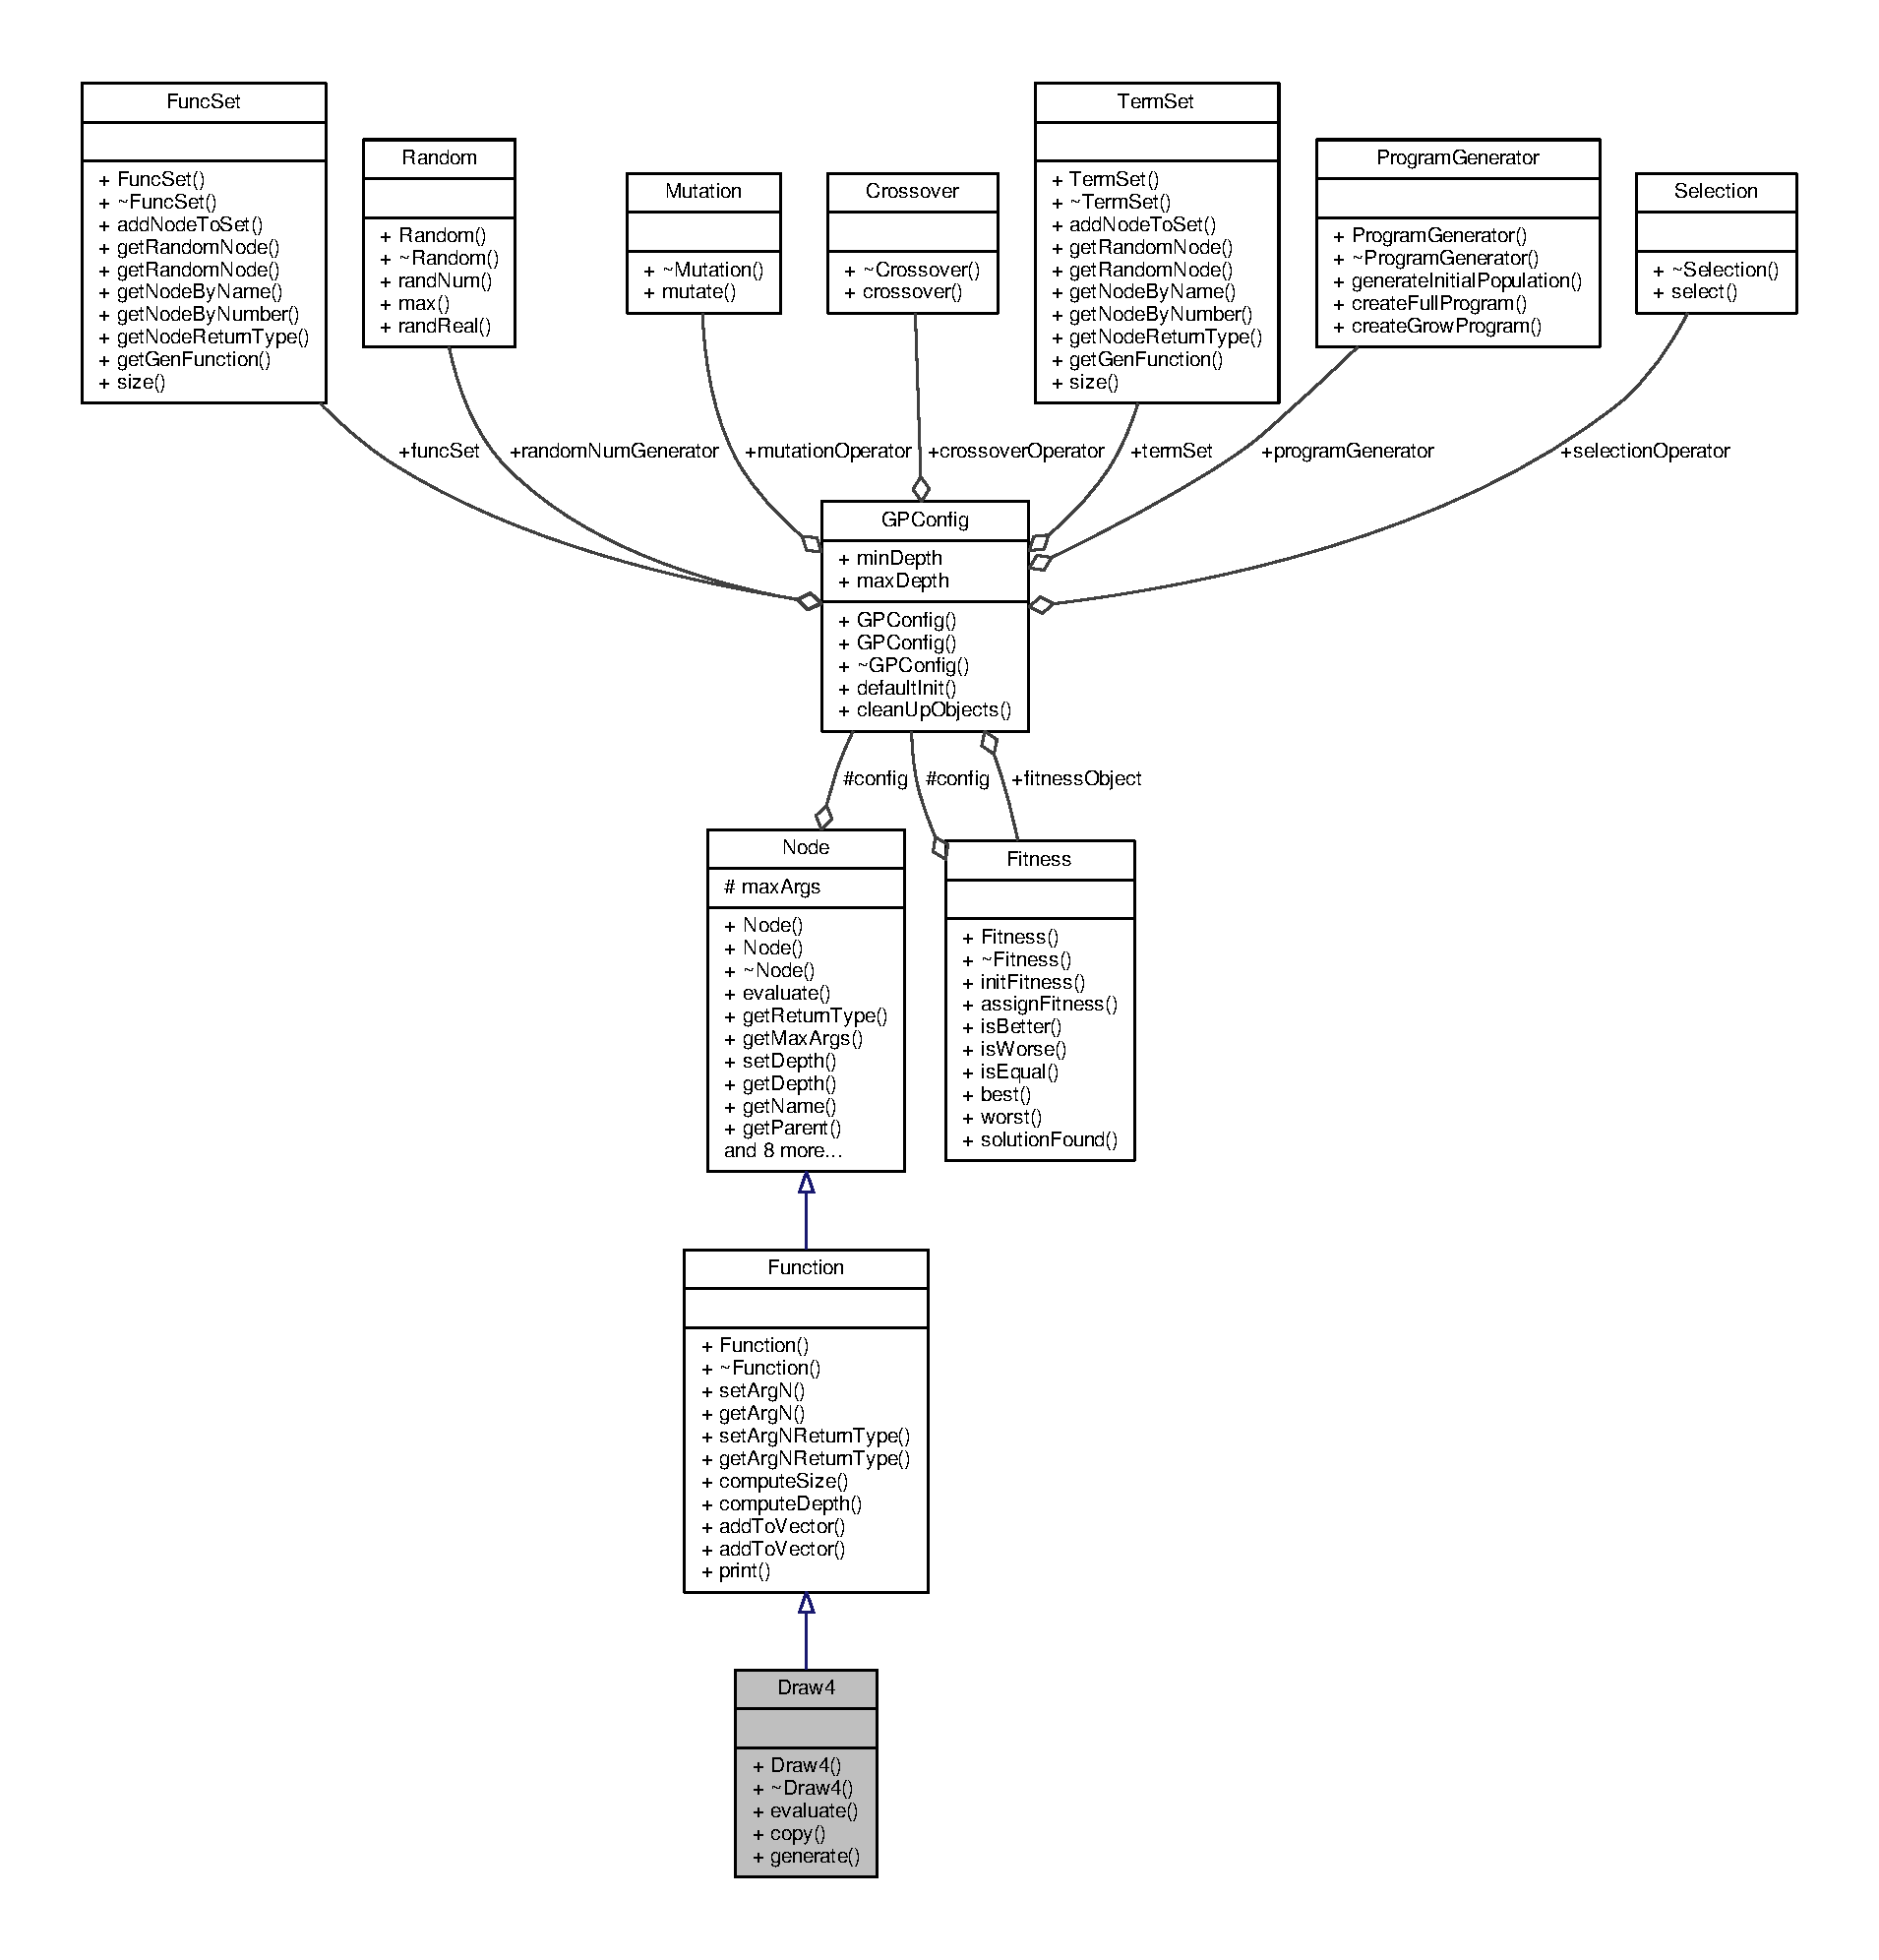
\includegraphics[width=350pt]{classDraw4__coll__graph}
\end{center}
\end{figure}
\subsection*{Public Member Functions}
\begin{DoxyCompactItemize}
\item 
\hypertarget{classDraw4_a30a878a94519eb6c291629927d5edf5d}{}\label{classDraw4_a30a878a94519eb6c291629927d5edf5d} 
{\bfseries Draw4} (\hyperlink{classGPConfig}{G\+P\+Config} $\ast$conf)
\item 
\hypertarget{classDraw4_a2eeefbe82ec2b6fef14e8bd5947c02ac}{}\label{classDraw4_a2eeefbe82ec2b6fef14e8bd5947c02ac} 
virtual void {\bfseries evaluate} (\hyperlink{classReturnData}{Return\+Data} $\ast$out)
\item 
\hypertarget{classDraw4_a6e4128cfa6b2b59dd08eb7e25da03f2e}{}\label{classDraw4_a6e4128cfa6b2b59dd08eb7e25da03f2e} 
virtual \hyperlink{classNode}{Node} $\ast$ {\bfseries copy} ()
\end{DoxyCompactItemize}
\subsection*{Static Public Member Functions}
\begin{DoxyCompactItemize}
\item 
\hypertarget{classDraw4_a125086be4643dd452fc5f952a61f9e83}{}\label{classDraw4_a125086be4643dd452fc5f952a61f9e83} 
static \hyperlink{classFunction}{Function} $\ast$ {\bfseries generate} (const string \&name, \hyperlink{classGPConfig}{G\+P\+Config} $\ast$conf)
\end{DoxyCompactItemize}
\subsection*{Additional Inherited Members}


The documentation for this class was generated from the following files\+:\begin{DoxyCompactItemize}
\item 
/home/\+Lach/npr-\/v109/src\+\_\+109/Draw4.\+h\item 
/home/\+Lach/npr-\/v109/src\+\_\+109/Draw4.\+cpp\end{DoxyCompactItemize}

\hypertarget{classDraw6}{}\section{Draw6 Class Reference}
\label{classDraw6}\index{Draw6@{Draw6}}


Inheritance diagram for Draw6\+:
\nopagebreak
\begin{figure}[H]
\begin{center}
\leavevmode
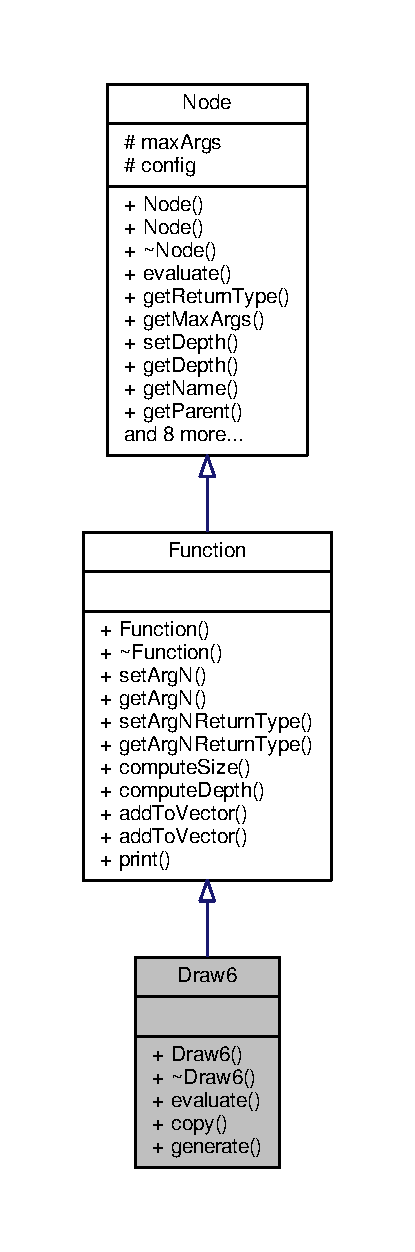
\includegraphics[height=550pt]{classDraw6__inherit__graph}
\end{center}
\end{figure}


Collaboration diagram for Draw6\+:
\nopagebreak
\begin{figure}[H]
\begin{center}
\leavevmode
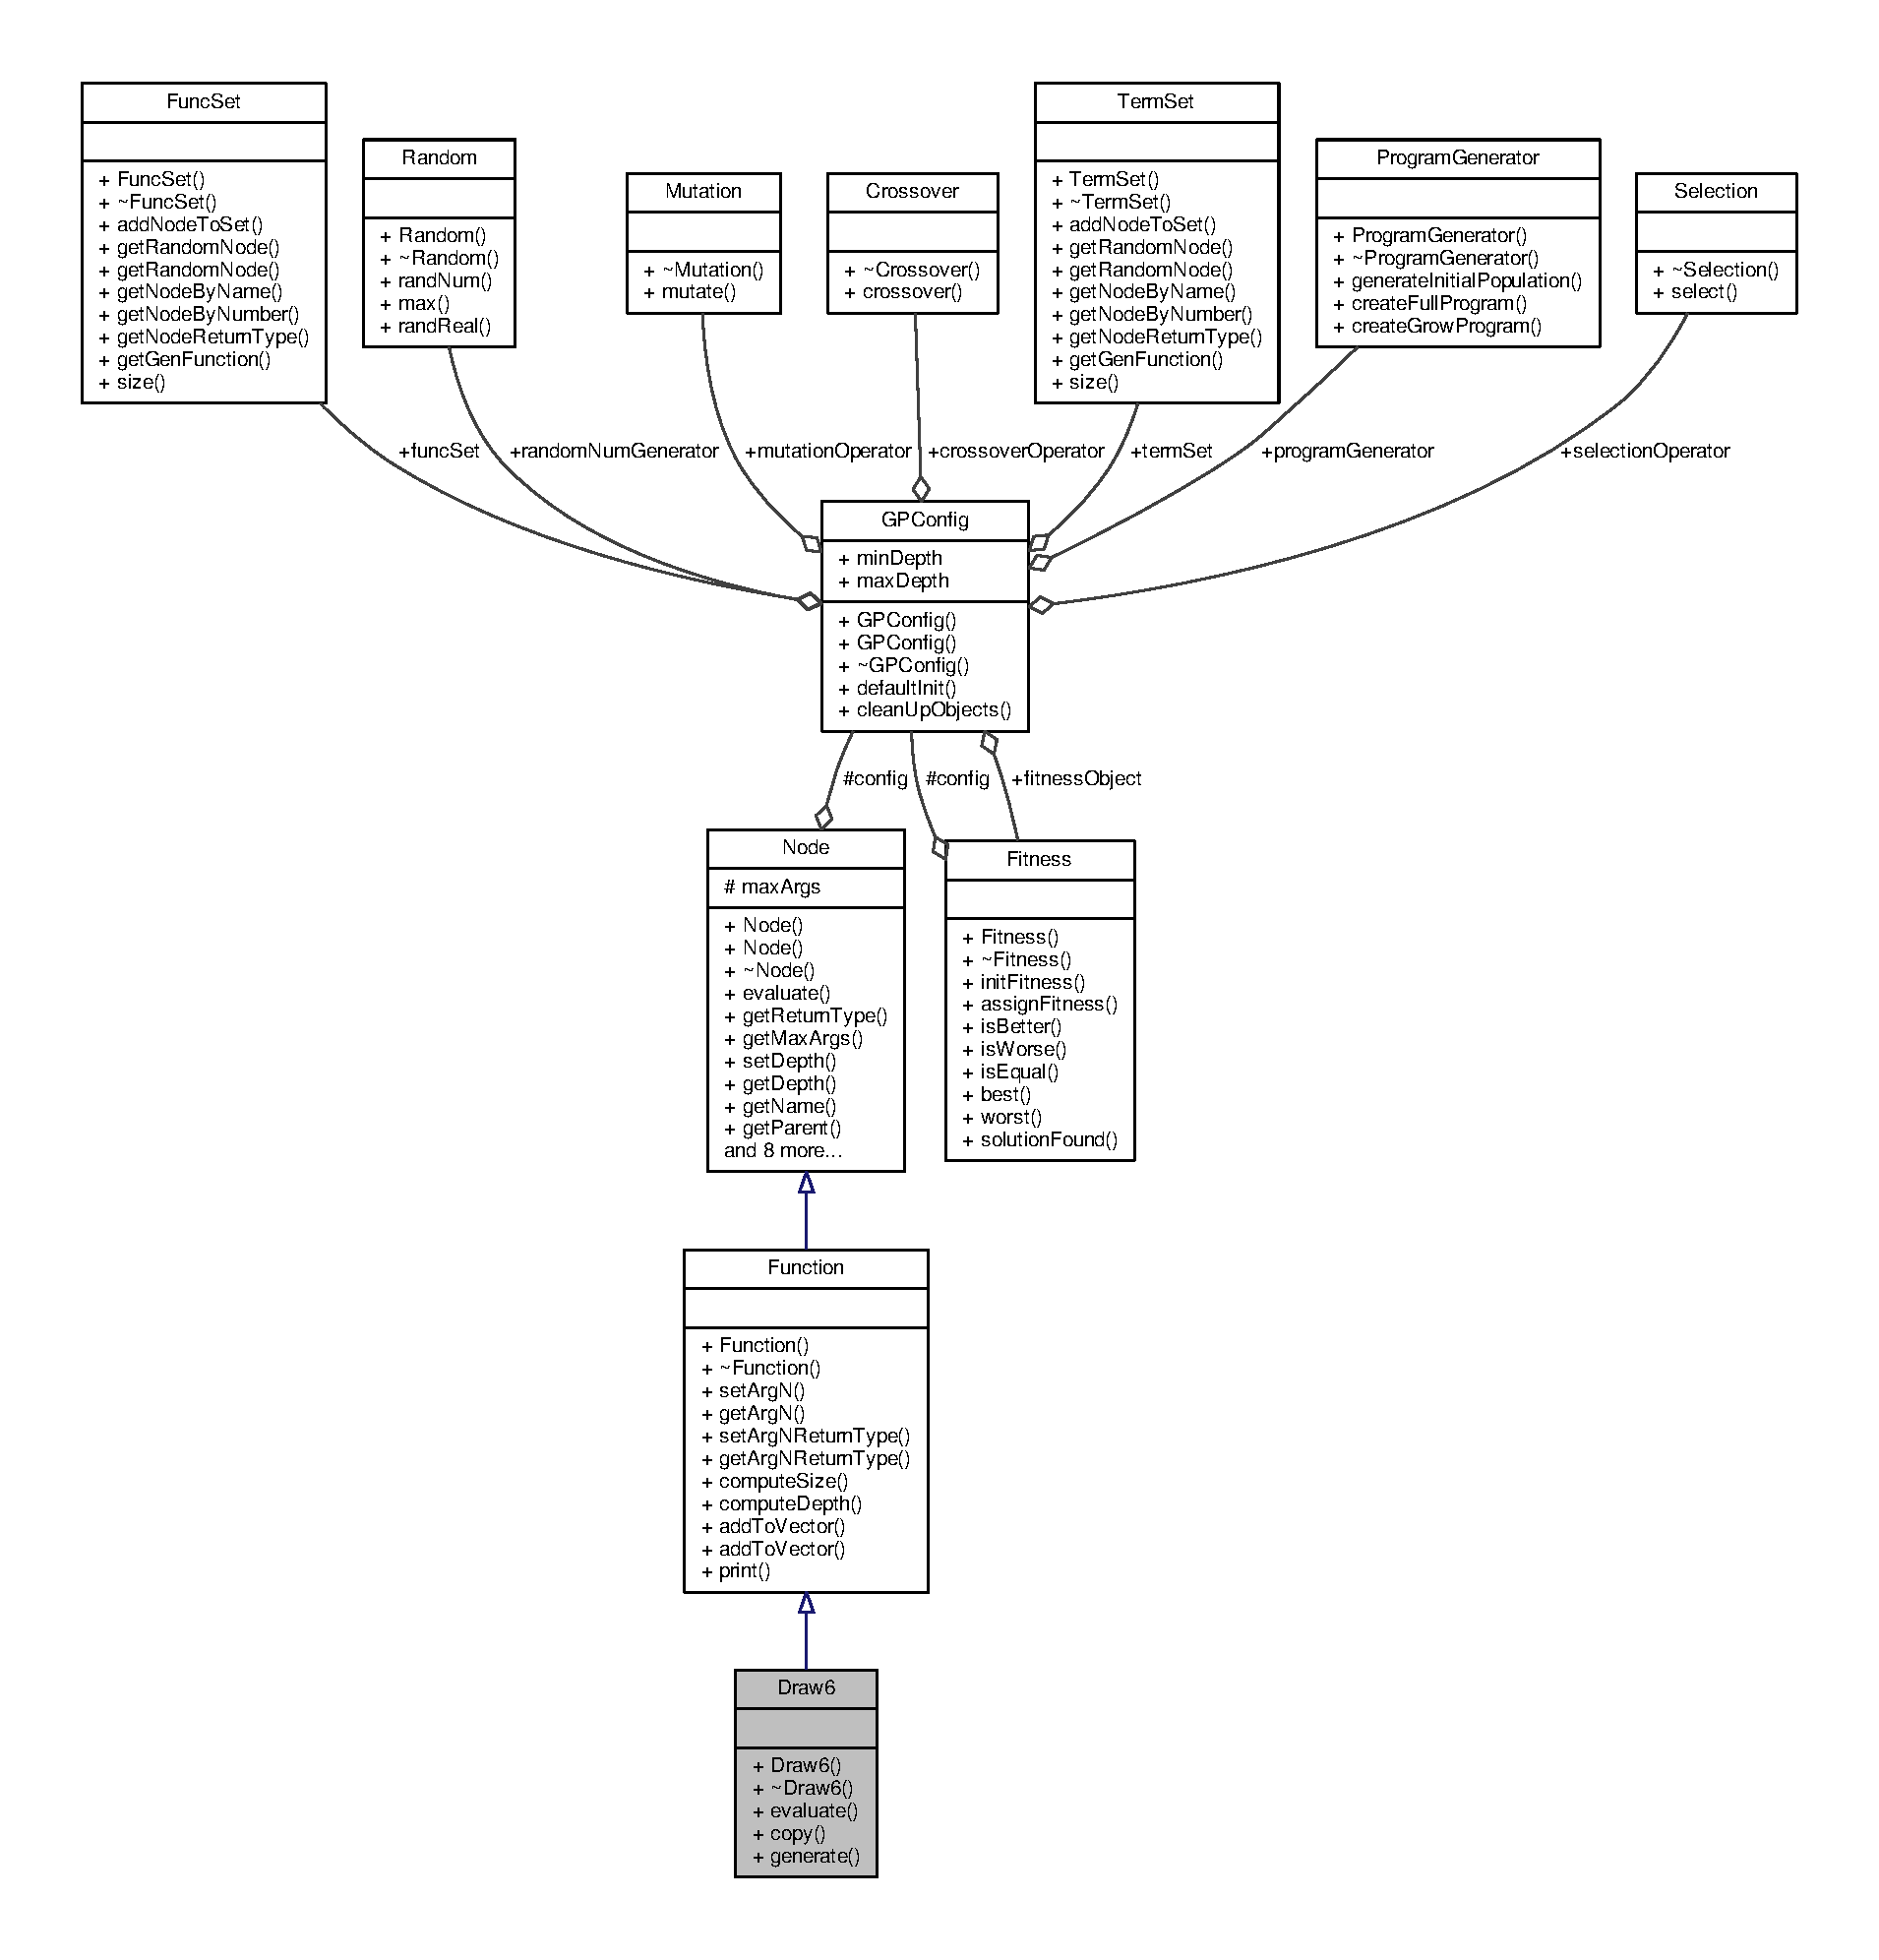
\includegraphics[width=350pt]{classDraw6__coll__graph}
\end{center}
\end{figure}
\subsection*{Public Member Functions}
\begin{DoxyCompactItemize}
\item 
\hypertarget{classDraw6_a3ce8484795df7bd08600ee8a7d457852}{}\label{classDraw6_a3ce8484795df7bd08600ee8a7d457852} 
{\bfseries Draw6} (\hyperlink{classGPConfig}{G\+P\+Config} $\ast$conf)
\item 
\hypertarget{classDraw6_afc1c9a9b88e1857dc72e9d92abe7a701}{}\label{classDraw6_afc1c9a9b88e1857dc72e9d92abe7a701} 
virtual void {\bfseries evaluate} (\hyperlink{classReturnData}{Return\+Data} $\ast$out)
\item 
\hypertarget{classDraw6_a005e2fba5cbe94cf402f242a05e86cd2}{}\label{classDraw6_a005e2fba5cbe94cf402f242a05e86cd2} 
virtual \hyperlink{classNode}{Node} $\ast$ {\bfseries copy} ()
\end{DoxyCompactItemize}
\subsection*{Static Public Member Functions}
\begin{DoxyCompactItemize}
\item 
\hypertarget{classDraw6_afc0f21375d2221fc5b558e7144e3e59d}{}\label{classDraw6_afc0f21375d2221fc5b558e7144e3e59d} 
static \hyperlink{classFunction}{Function} $\ast$ {\bfseries generate} (const string \&name, \hyperlink{classGPConfig}{G\+P\+Config} $\ast$conf)
\end{DoxyCompactItemize}
\subsection*{Additional Inherited Members}


The documentation for this class was generated from the following files\+:\begin{DoxyCompactItemize}
\item 
/home/\+Lach/npr-\/v109/src\+\_\+109/Draw6.\+h\item 
/home/\+Lach/npr-\/v109/src\+\_\+109/Draw6.\+cpp\end{DoxyCompactItemize}

\hypertarget{classDrawColorTriangle}{}\section{Draw\+Color\+Triangle Class Reference}
\label{classDrawColorTriangle}\index{Draw\+Color\+Triangle@{Draw\+Color\+Triangle}}


Inheritance diagram for Draw\+Color\+Triangle\+:
\nopagebreak
\begin{figure}[H]
\begin{center}
\leavevmode
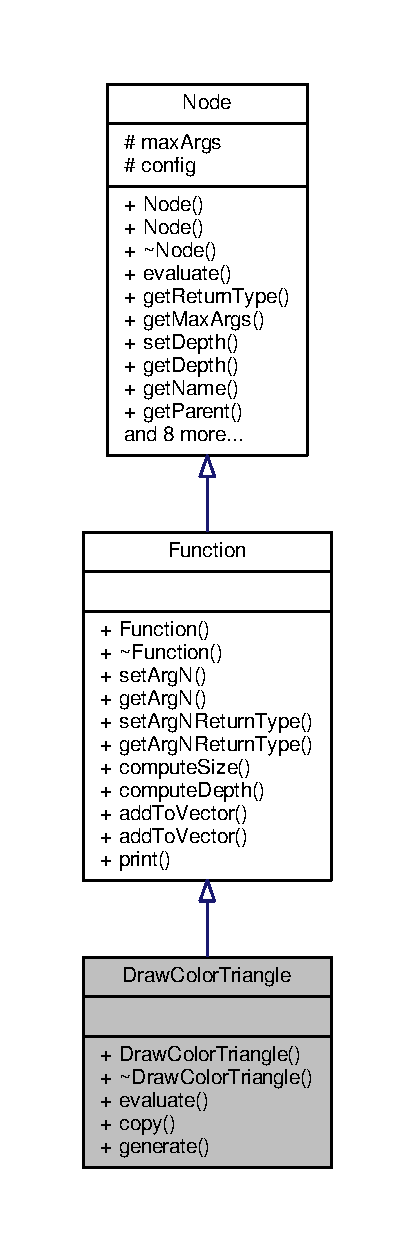
\includegraphics[height=550pt]{classDrawColorTriangle__inherit__graph}
\end{center}
\end{figure}


Collaboration diagram for Draw\+Color\+Triangle\+:
\nopagebreak
\begin{figure}[H]
\begin{center}
\leavevmode
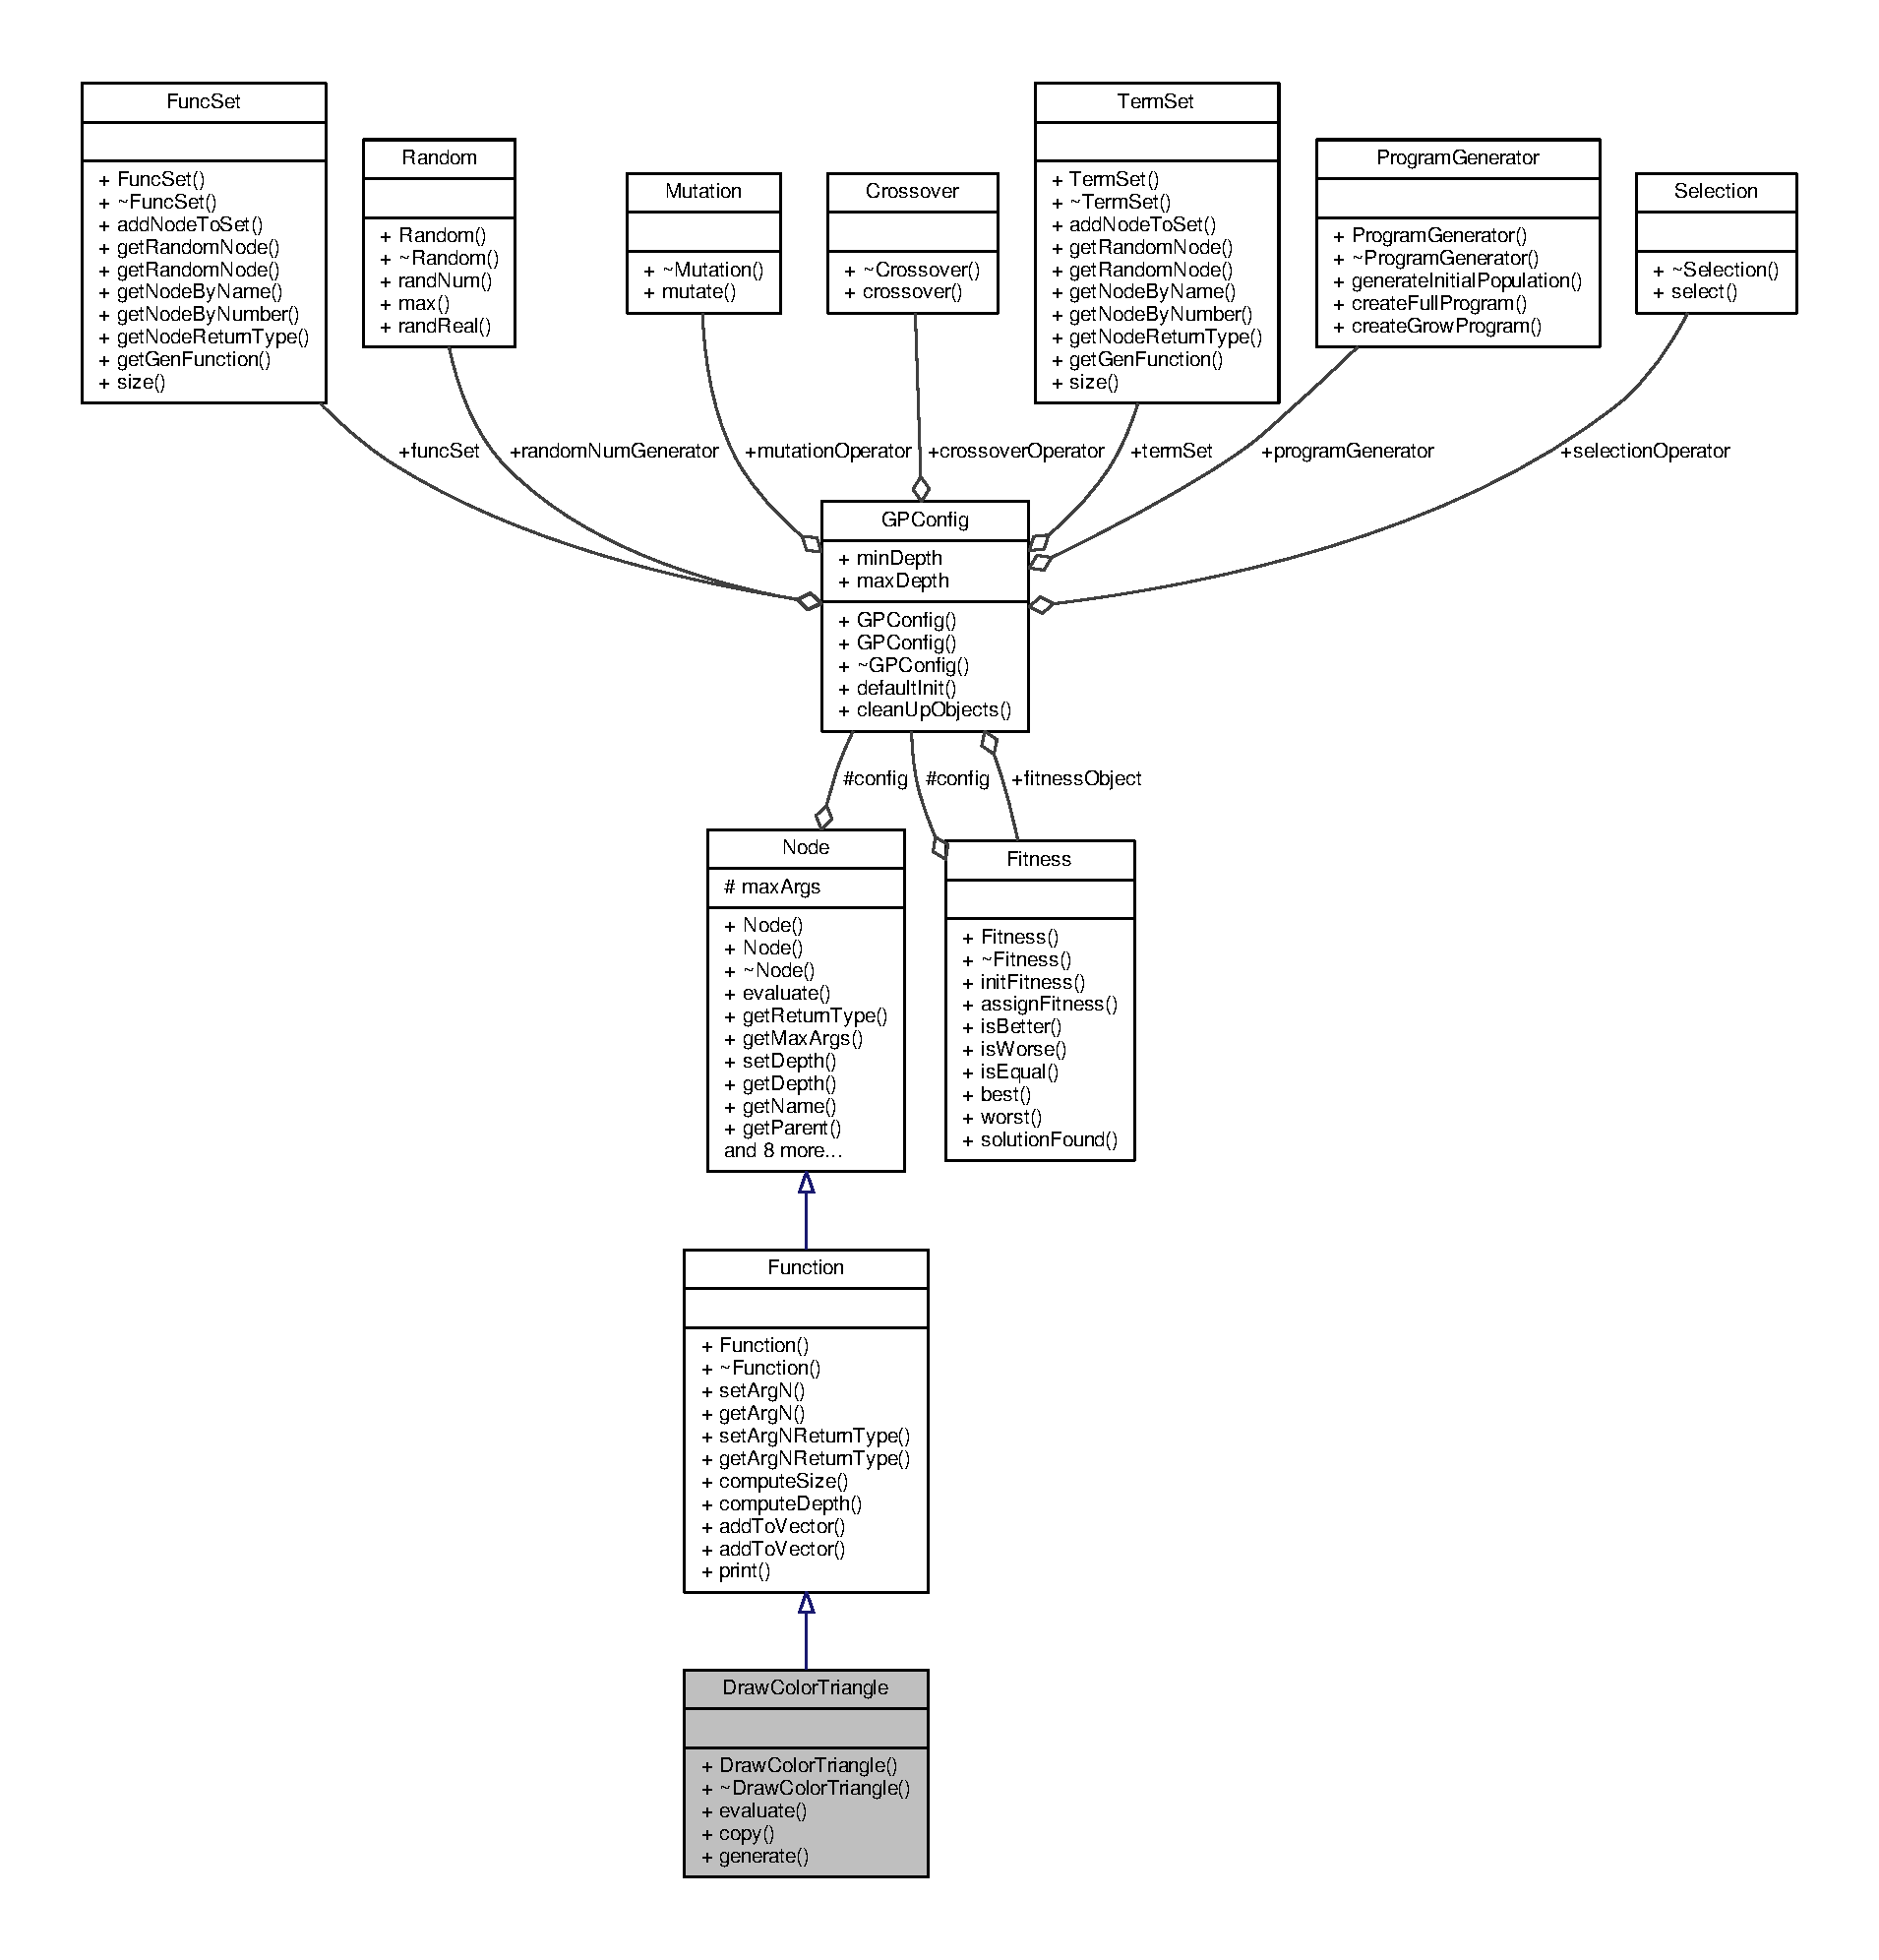
\includegraphics[width=350pt]{classDrawColorTriangle__coll__graph}
\end{center}
\end{figure}
\subsection*{Public Member Functions}
\begin{DoxyCompactItemize}
\item 
\hypertarget{classDrawColorTriangle_a0bbb6e498405631981f2af8c30bed2a3}{}\label{classDrawColorTriangle_a0bbb6e498405631981f2af8c30bed2a3} 
{\bfseries Draw\+Color\+Triangle} (\hyperlink{classGPConfig}{G\+P\+Config} $\ast$conf)
\item 
\hypertarget{classDrawColorTriangle_a015d98a34270b2e0d50abc398cec39e3}{}\label{classDrawColorTriangle_a015d98a34270b2e0d50abc398cec39e3} 
virtual void {\bfseries evaluate} (\hyperlink{classReturnData}{Return\+Data} $\ast$out)
\item 
\hypertarget{classDrawColorTriangle_a8854b0eedda24cb7e68088ea04fa3d31}{}\label{classDrawColorTriangle_a8854b0eedda24cb7e68088ea04fa3d31} 
virtual \hyperlink{classNode}{Node} $\ast$ {\bfseries copy} ()
\end{DoxyCompactItemize}
\subsection*{Static Public Member Functions}
\begin{DoxyCompactItemize}
\item 
\hypertarget{classDrawColorTriangle_aafd3098c23fae0a80e8aae9297b9e490}{}\label{classDrawColorTriangle_aafd3098c23fae0a80e8aae9297b9e490} 
static \hyperlink{classFunction}{Function} $\ast$ {\bfseries generate} (const string \&name, \hyperlink{classGPConfig}{G\+P\+Config} $\ast$conf)
\end{DoxyCompactItemize}
\subsection*{Additional Inherited Members}


The documentation for this class was generated from the following files\+:\begin{DoxyCompactItemize}
\item 
/home/\+Lach/npr-\/v109/src\+\_\+109/Draw\+Color\+Triangle.\+h\item 
/home/\+Lach/npr-\/v109/src\+\_\+109/Draw\+Color\+Triangle.\+cpp\end{DoxyCompactItemize}

\hypertarget{classDrawGrayTriangle}{}\section{Draw\+Gray\+Triangle Class Reference}
\label{classDrawGrayTriangle}\index{Draw\+Gray\+Triangle@{Draw\+Gray\+Triangle}}


Inheritance diagram for Draw\+Gray\+Triangle\+:
\nopagebreak
\begin{figure}[H]
\begin{center}
\leavevmode
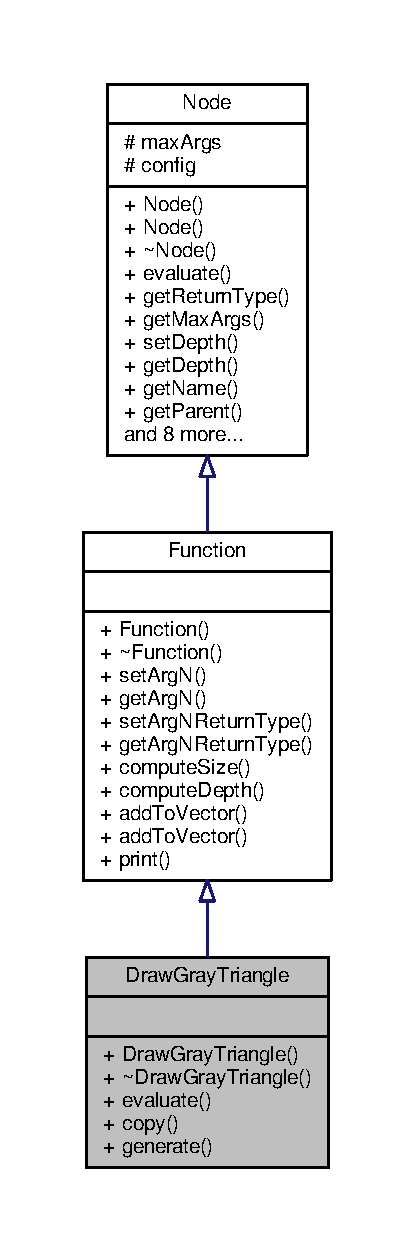
\includegraphics[height=550pt]{classDrawGrayTriangle__inherit__graph}
\end{center}
\end{figure}


Collaboration diagram for Draw\+Gray\+Triangle\+:
\nopagebreak
\begin{figure}[H]
\begin{center}
\leavevmode
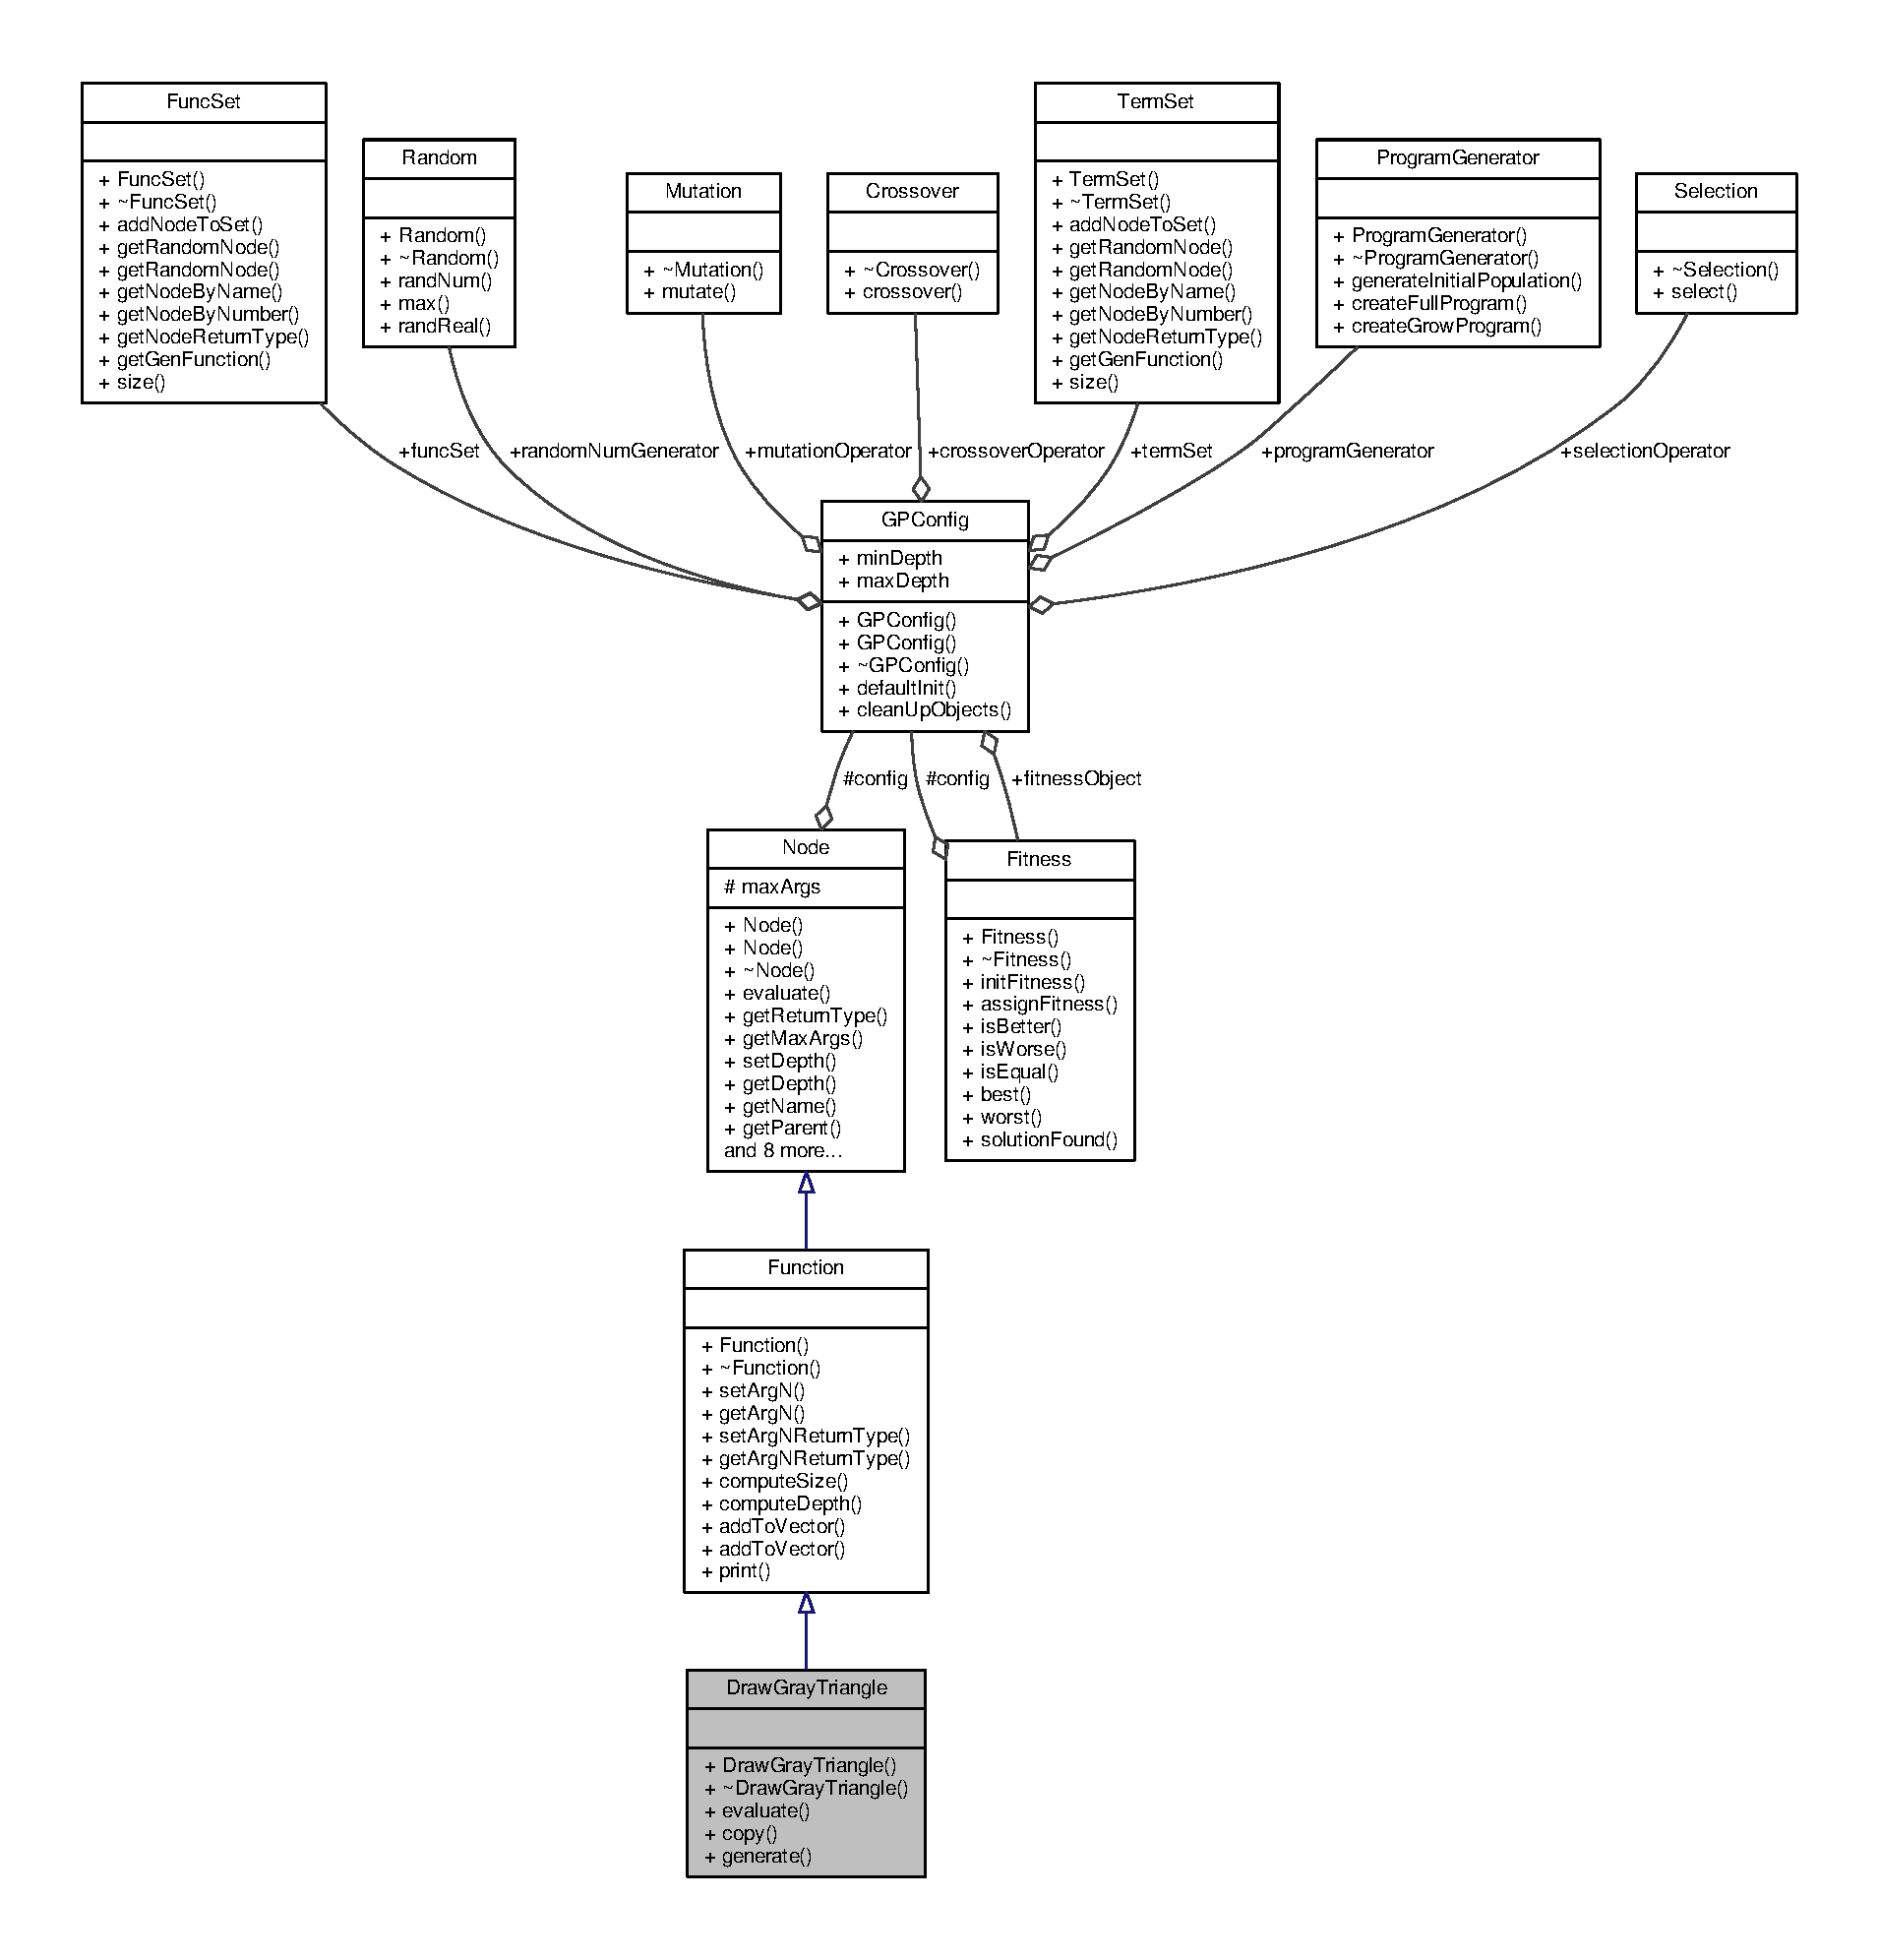
\includegraphics[width=350pt]{classDrawGrayTriangle__coll__graph}
\end{center}
\end{figure}
\subsection*{Public Member Functions}
\begin{DoxyCompactItemize}
\item 
\hypertarget{classDrawGrayTriangle_a7a518e20ef8d09167ce78beb13c736cd}{}\label{classDrawGrayTriangle_a7a518e20ef8d09167ce78beb13c736cd} 
{\bfseries Draw\+Gray\+Triangle} (\hyperlink{classGPConfig}{G\+P\+Config} $\ast$conf)
\item 
\hypertarget{classDrawGrayTriangle_a17a78c3748736ef48dc8951b07361e68}{}\label{classDrawGrayTriangle_a17a78c3748736ef48dc8951b07361e68} 
virtual void {\bfseries evaluate} (\hyperlink{classReturnData}{Return\+Data} $\ast$out)
\item 
\hypertarget{classDrawGrayTriangle_a085f4c505bbb6ff6e129649f29917276}{}\label{classDrawGrayTriangle_a085f4c505bbb6ff6e129649f29917276} 
virtual \hyperlink{classNode}{Node} $\ast$ {\bfseries copy} ()
\end{DoxyCompactItemize}
\subsection*{Static Public Member Functions}
\begin{DoxyCompactItemize}
\item 
\hypertarget{classDrawGrayTriangle_ac9f2292e5d9b3709bb4f5fbb80a73e25}{}\label{classDrawGrayTriangle_ac9f2292e5d9b3709bb4f5fbb80a73e25} 
static \hyperlink{classFunction}{Function} $\ast$ {\bfseries generate} (const string \&name, \hyperlink{classGPConfig}{G\+P\+Config} $\ast$conf)
\end{DoxyCompactItemize}
\subsection*{Additional Inherited Members}


The documentation for this class was generated from the following files\+:\begin{DoxyCompactItemize}
\item 
/home/\+Lach/npr-\/v109/src\+\_\+109/Draw\+Gray\+Triangle.\+h\item 
/home/\+Lach/npr-\/v109/src\+\_\+109/Draw\+Gray\+Triangle.\+cpp\end{DoxyCompactItemize}

\hypertarget{classNodeVector_1_1Element}{}\section{Node\+Vector$<$ Type $>$\+:\+:Element Class Reference}
\label{classNodeVector_1_1Element}\index{Node\+Vector$<$ Type $>$\+::\+Element@{Node\+Vector$<$ Type $>$\+::\+Element}}


Collaboration diagram for Node\+Vector$<$ Type $>$\+:\+:Element\+:
\nopagebreak
\begin{figure}[H]
\begin{center}
\leavevmode
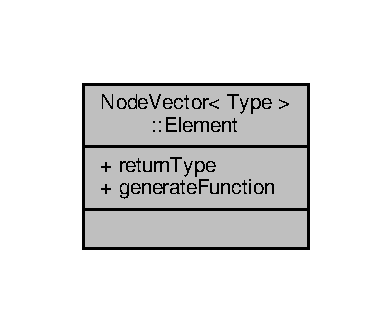
\includegraphics[width=188pt]{classNodeVector_1_1Element__coll__graph}
\end{center}
\end{figure}
\subsection*{Public Attributes}
\begin{DoxyCompactItemize}
\item 
\hypertarget{classNodeVector_1_1Element_a75e5f7179322ec4c3f6b9b62318c2c38}{}\label{classNodeVector_1_1Element_a75e5f7179322ec4c3f6b9b62318c2c38} 
int {\bfseries return\+Type}
\item 
\hypertarget{classNodeVector_1_1Element_a9835441c75670f207457aa1a167fbd37}{}\label{classNodeVector_1_1Element_a9835441c75670f207457aa1a167fbd37} 
Type $\ast$($\ast$ {\bfseries generate\+Function} )(const string \&, \hyperlink{classGPConfig}{G\+P\+Config} $\ast$)
\end{DoxyCompactItemize}


The documentation for this class was generated from the following file\+:\begin{DoxyCompactItemize}
\item 
/home/\+Lach/npr-\/v109/\+R\+M\+I\+T\+G\+P.\+1.\+5/Node\+Vector.\+h\end{DoxyCompactItemize}

\hypertarget{classFitness}{}\section{Fitness Class Reference}
\label{classFitness}\index{Fitness@{Fitness}}


Inheritance diagram for Fitness\+:
\nopagebreak
\begin{figure}[H]
\begin{center}
\leavevmode
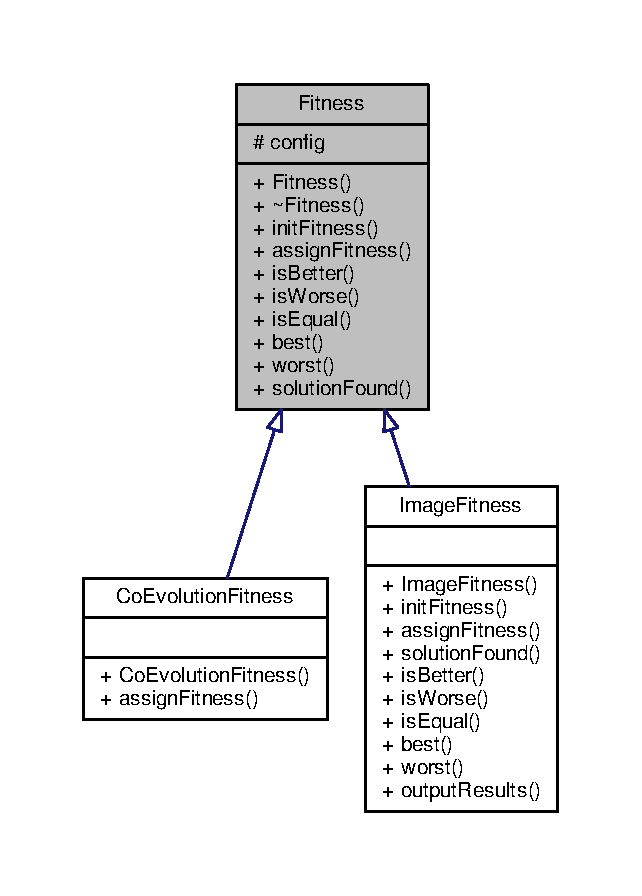
\includegraphics[width=308pt]{classFitness__inherit__graph}
\end{center}
\end{figure}


Collaboration diagram for Fitness\+:
\nopagebreak
\begin{figure}[H]
\begin{center}
\leavevmode
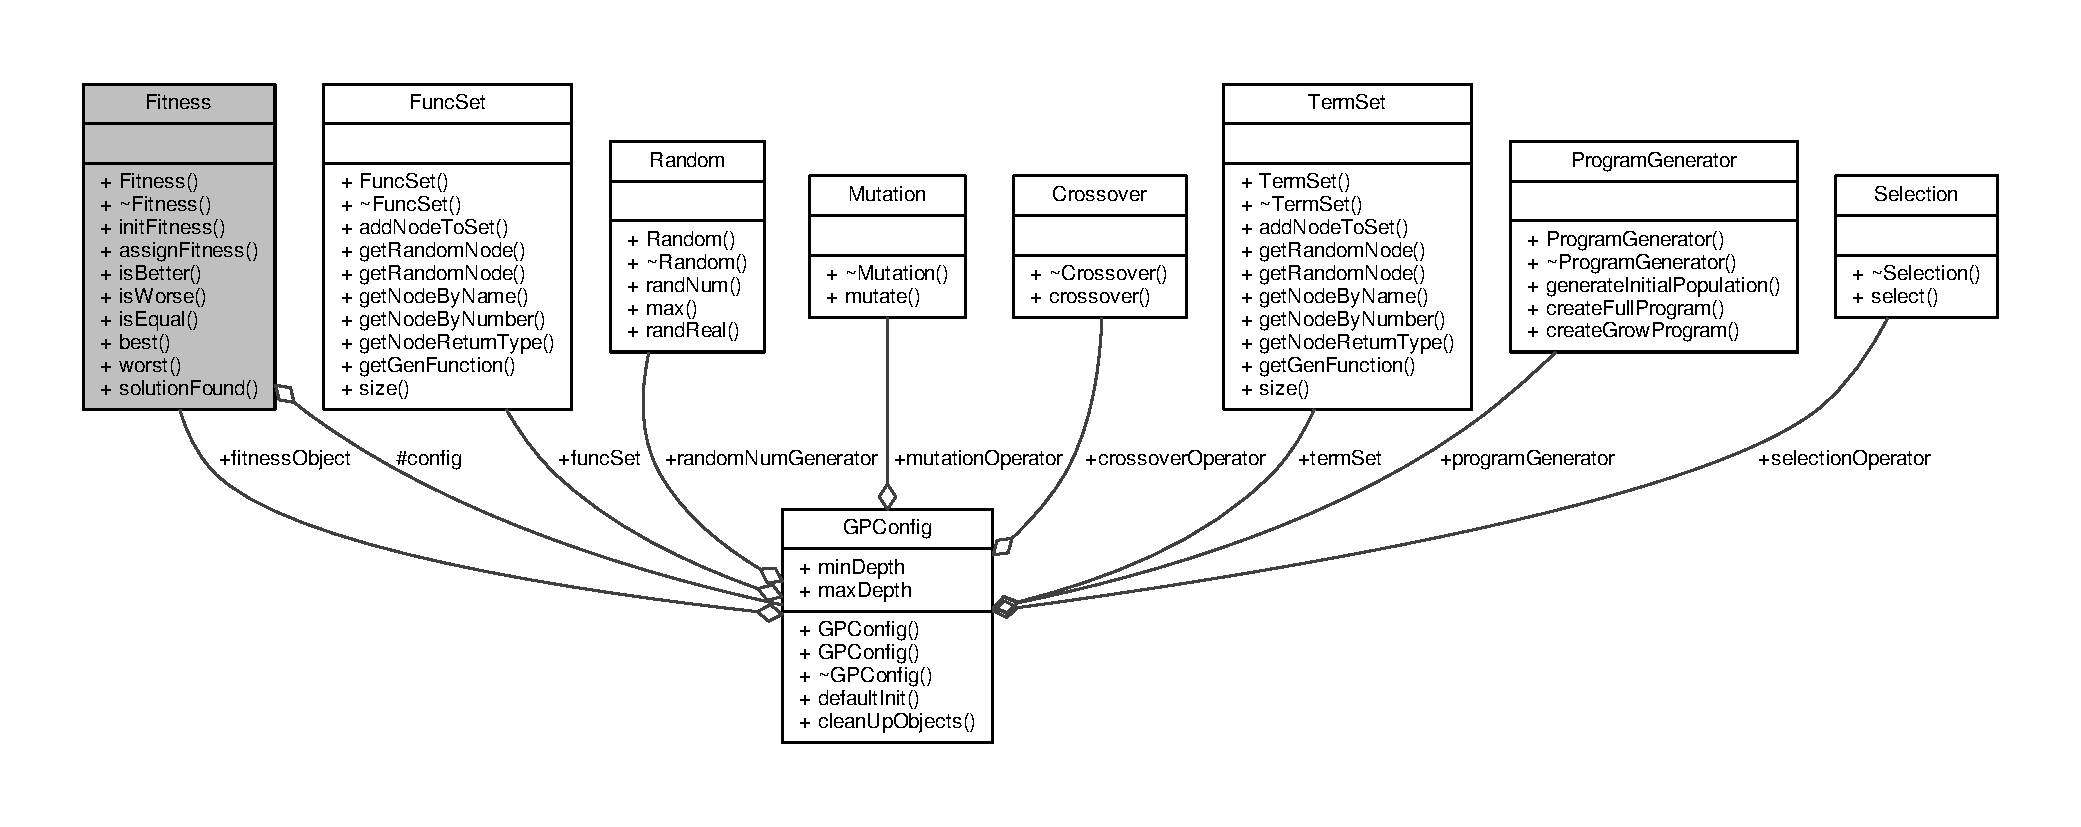
\includegraphics[width=350pt]{classFitness__coll__graph}
\end{center}
\end{figure}
\subsection*{Public Member Functions}
\begin{DoxyCompactItemize}
\item 
\hypertarget{classFitness_ae7a108ef7b21c86d21edc1d65fb94791}{}\label{classFitness_ae7a108ef7b21c86d21edc1d65fb94791} 
{\bfseries Fitness} (\hyperlink{classGPConfig}{G\+P\+Config} $\ast$conf)
\item 
\hypertarget{classFitness_af0cc76842533549497d736317291adeb}{}\label{classFitness_af0cc76842533549497d736317291adeb} 
virtual void {\bfseries init\+Fitness} ()=0
\item 
\hypertarget{classFitness_ad0204160e312a1949c92dbe97dc45283}{}\label{classFitness_ad0204160e312a1949c92dbe97dc45283} 
virtual void {\bfseries assign\+Fitness} (\hyperlink{classGeneticProgram}{Genetic\+Program} $\ast$pop\mbox{[}$\,$\mbox{]}, int pop\+Size)=0
\item 
\hypertarget{classFitness_ad0121622fdd110ac1da209c000ec0efa}{}\label{classFitness_ad0121622fdd110ac1da209c000ec0efa} 
virtual bool {\bfseries is\+Better} (\hyperlink{classGeneticProgram}{Genetic\+Program} $\ast$gp1, \hyperlink{classGeneticProgram}{Genetic\+Program} $\ast$gp2)=0
\item 
\hypertarget{classFitness_a0faa716e3afd9de0580ed7526b7eeed3}{}\label{classFitness_a0faa716e3afd9de0580ed7526b7eeed3} 
virtual bool {\bfseries is\+Worse} (\hyperlink{classGeneticProgram}{Genetic\+Program} $\ast$gp1, \hyperlink{classGeneticProgram}{Genetic\+Program} $\ast$gp2)=0
\item 
\hypertarget{classFitness_acd0b1070998ce9c8f1522f0107cc81e8}{}\label{classFitness_acd0b1070998ce9c8f1522f0107cc81e8} 
virtual bool {\bfseries is\+Equal} (\hyperlink{classGeneticProgram}{Genetic\+Program} $\ast$gp1, \hyperlink{classGeneticProgram}{Genetic\+Program} $\ast$gp2)=0
\item 
\hypertarget{classFitness_a6d16f5fa00718ec77703a16cdde52bba}{}\label{classFitness_a6d16f5fa00718ec77703a16cdde52bba} 
virtual double {\bfseries best} ()=0
\item 
\hypertarget{classFitness_a826f973a29bf98da811315b77c4c3710}{}\label{classFitness_a826f973a29bf98da811315b77c4c3710} 
virtual double {\bfseries worst} ()=0
\item 
\hypertarget{classFitness_a580a796f63acf4afdcb9061c484692c0}{}\label{classFitness_a580a796f63acf4afdcb9061c484692c0} 
virtual bool {\bfseries solution\+Found} (\hyperlink{classGeneticProgram}{Genetic\+Program} $\ast$pop\mbox{[}$\,$\mbox{]}, int pop\+Size)=0
\end{DoxyCompactItemize}
\subsection*{Protected Attributes}
\begin{DoxyCompactItemize}
\item 
\hypertarget{classFitness_af8b8f65772f11313377f15acfcba8ec3}{}\label{classFitness_af8b8f65772f11313377f15acfcba8ec3} 
\hyperlink{classGPConfig}{G\+P\+Config} $\ast$ {\bfseries config}
\end{DoxyCompactItemize}


The documentation for this class was generated from the following files\+:\begin{DoxyCompactItemize}
\item 
/home/\+Lach/npr-\/v109/\+R\+M\+I\+T\+G\+P.\+1.\+5/Fitness.\+h\item 
/home/\+Lach/npr-\/v109/\+R\+M\+I\+T\+G\+P.\+1.\+5/Fitness.\+cpp\end{DoxyCompactItemize}

\hypertarget{classFuncSet}{}\section{Func\+Set Class Reference}
\label{classFuncSet}\index{Func\+Set@{Func\+Set}}


Collaboration diagram for Func\+Set\+:
\nopagebreak
\begin{figure}[H]
\begin{center}
\leavevmode
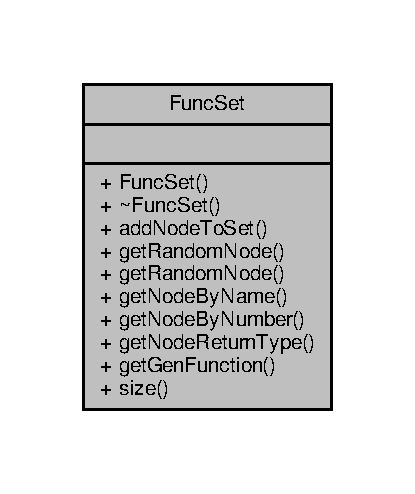
\includegraphics[width=199pt]{classFuncSet__coll__graph}
\end{center}
\end{figure}
\subsection*{Public Member Functions}
\begin{DoxyCompactItemize}
\item 
\hypertarget{classFuncSet_af38d587fdf20c058935cf7be826c4459}{}\label{classFuncSet_af38d587fdf20c058935cf7be826c4459} 
{\bfseries Func\+Set} (\hyperlink{classGPConfig}{G\+P\+Config} $\ast$conf)
\item 
\hypertarget{classFuncSet_a488cdd01ffacf8fe6d4081a56cf48285}{}\label{classFuncSet_a488cdd01ffacf8fe6d4081a56cf48285} 
void {\bfseries add\+Node\+To\+Set} (int return\+Type, \hyperlink{classFunction}{Function} $\ast$($\ast$generate\+Function)(const string \&, \hyperlink{classGPConfig}{G\+P\+Config} $\ast$))
\item 
\hypertarget{classFuncSet_a7ba39dff0e351c1b23dcd7de77065178}{}\label{classFuncSet_a7ba39dff0e351c1b23dcd7de77065178} 
\hyperlink{classFunction}{Function} $\ast$ {\bfseries get\+Random\+Node} ()
\item 
\hypertarget{classFuncSet_a56a52e61e2aeafea1bb012e4ab161307}{}\label{classFuncSet_a56a52e61e2aeafea1bb012e4ab161307} 
\hyperlink{classFunction}{Function} $\ast$ {\bfseries get\+Random\+Node} (int return\+Type)
\item 
\hypertarget{classFuncSet_a9b115eb0e18850a4ee8c81102eb7c491}{}\label{classFuncSet_a9b115eb0e18850a4ee8c81102eb7c491} 
\hyperlink{classNode}{Node} $\ast$ {\bfseries get\+Node\+By\+Name} (const string \&name)
\item 
\hypertarget{classFuncSet_adaa6674456af8906a05fa1e861e16cf4}{}\label{classFuncSet_adaa6674456af8906a05fa1e861e16cf4} 
\hyperlink{classNode}{Node} $\ast$ {\bfseries get\+Node\+By\+Number} (int position)
\item 
\hypertarget{classFuncSet_a3e346c9bed6d63bb77a4005f1cf90fc1}{}\label{classFuncSet_a3e346c9bed6d63bb77a4005f1cf90fc1} 
int {\bfseries get\+Node\+Return\+Type} (int position)
\item 
\hypertarget{classFuncSet_ac0e0a59155d2d9bf384b6094d8dde7d9}{}\label{classFuncSet_ac0e0a59155d2d9bf384b6094d8dde7d9} 
func\+Gen {\bfseries get\+Gen\+Function} (int position)
\item 
\hypertarget{classFuncSet_a018edfe8710687117b9f40619c867200}{}\label{classFuncSet_a018edfe8710687117b9f40619c867200} 
int {\bfseries size} () const
\end{DoxyCompactItemize}


The documentation for this class was generated from the following files\+:\begin{DoxyCompactItemize}
\item 
/home/\+Lach/npr-\/v109/\+R\+M\+I\+T\+G\+P.\+1.\+5/Node\+Set.\+h\item 
/home/\+Lach/npr-\/v109/\+R\+M\+I\+T\+G\+P.\+1.\+5/Node\+Set.\+cpp\end{DoxyCompactItemize}

\hypertarget{classFunction}{}\section{Function Class Reference}
\label{classFunction}\index{Function@{Function}}


Inheritance diagram for Function\+:
\nopagebreak
\begin{figure}[H]
\begin{center}
\leavevmode
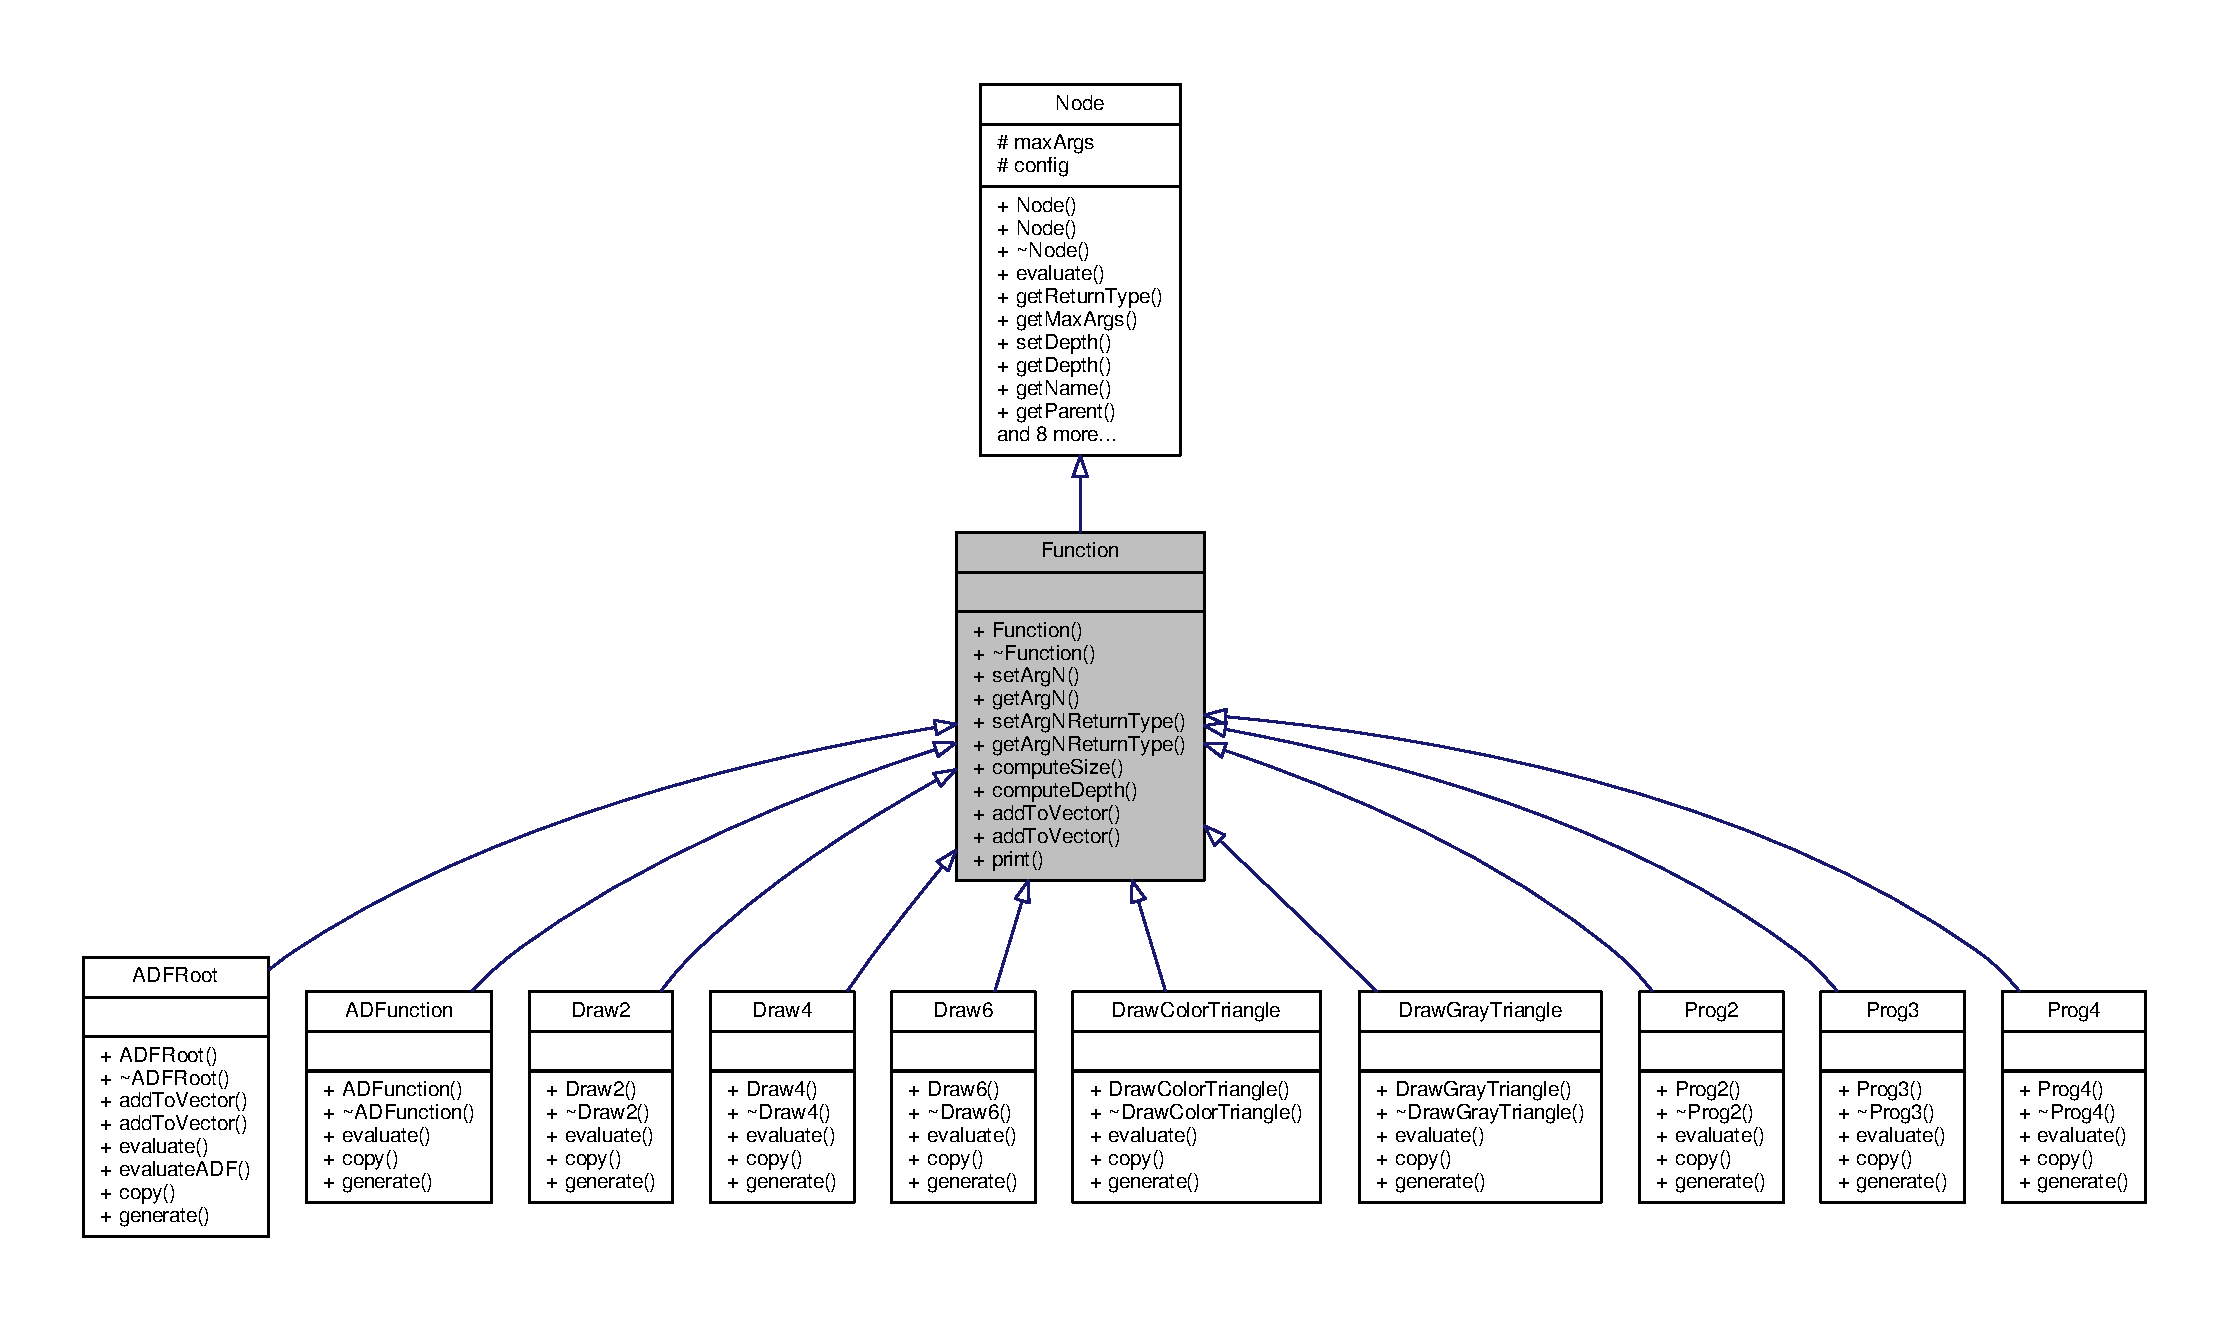
\includegraphics[width=350pt]{classFunction__inherit__graph}
\end{center}
\end{figure}


Collaboration diagram for Function\+:
\nopagebreak
\begin{figure}[H]
\begin{center}
\leavevmode
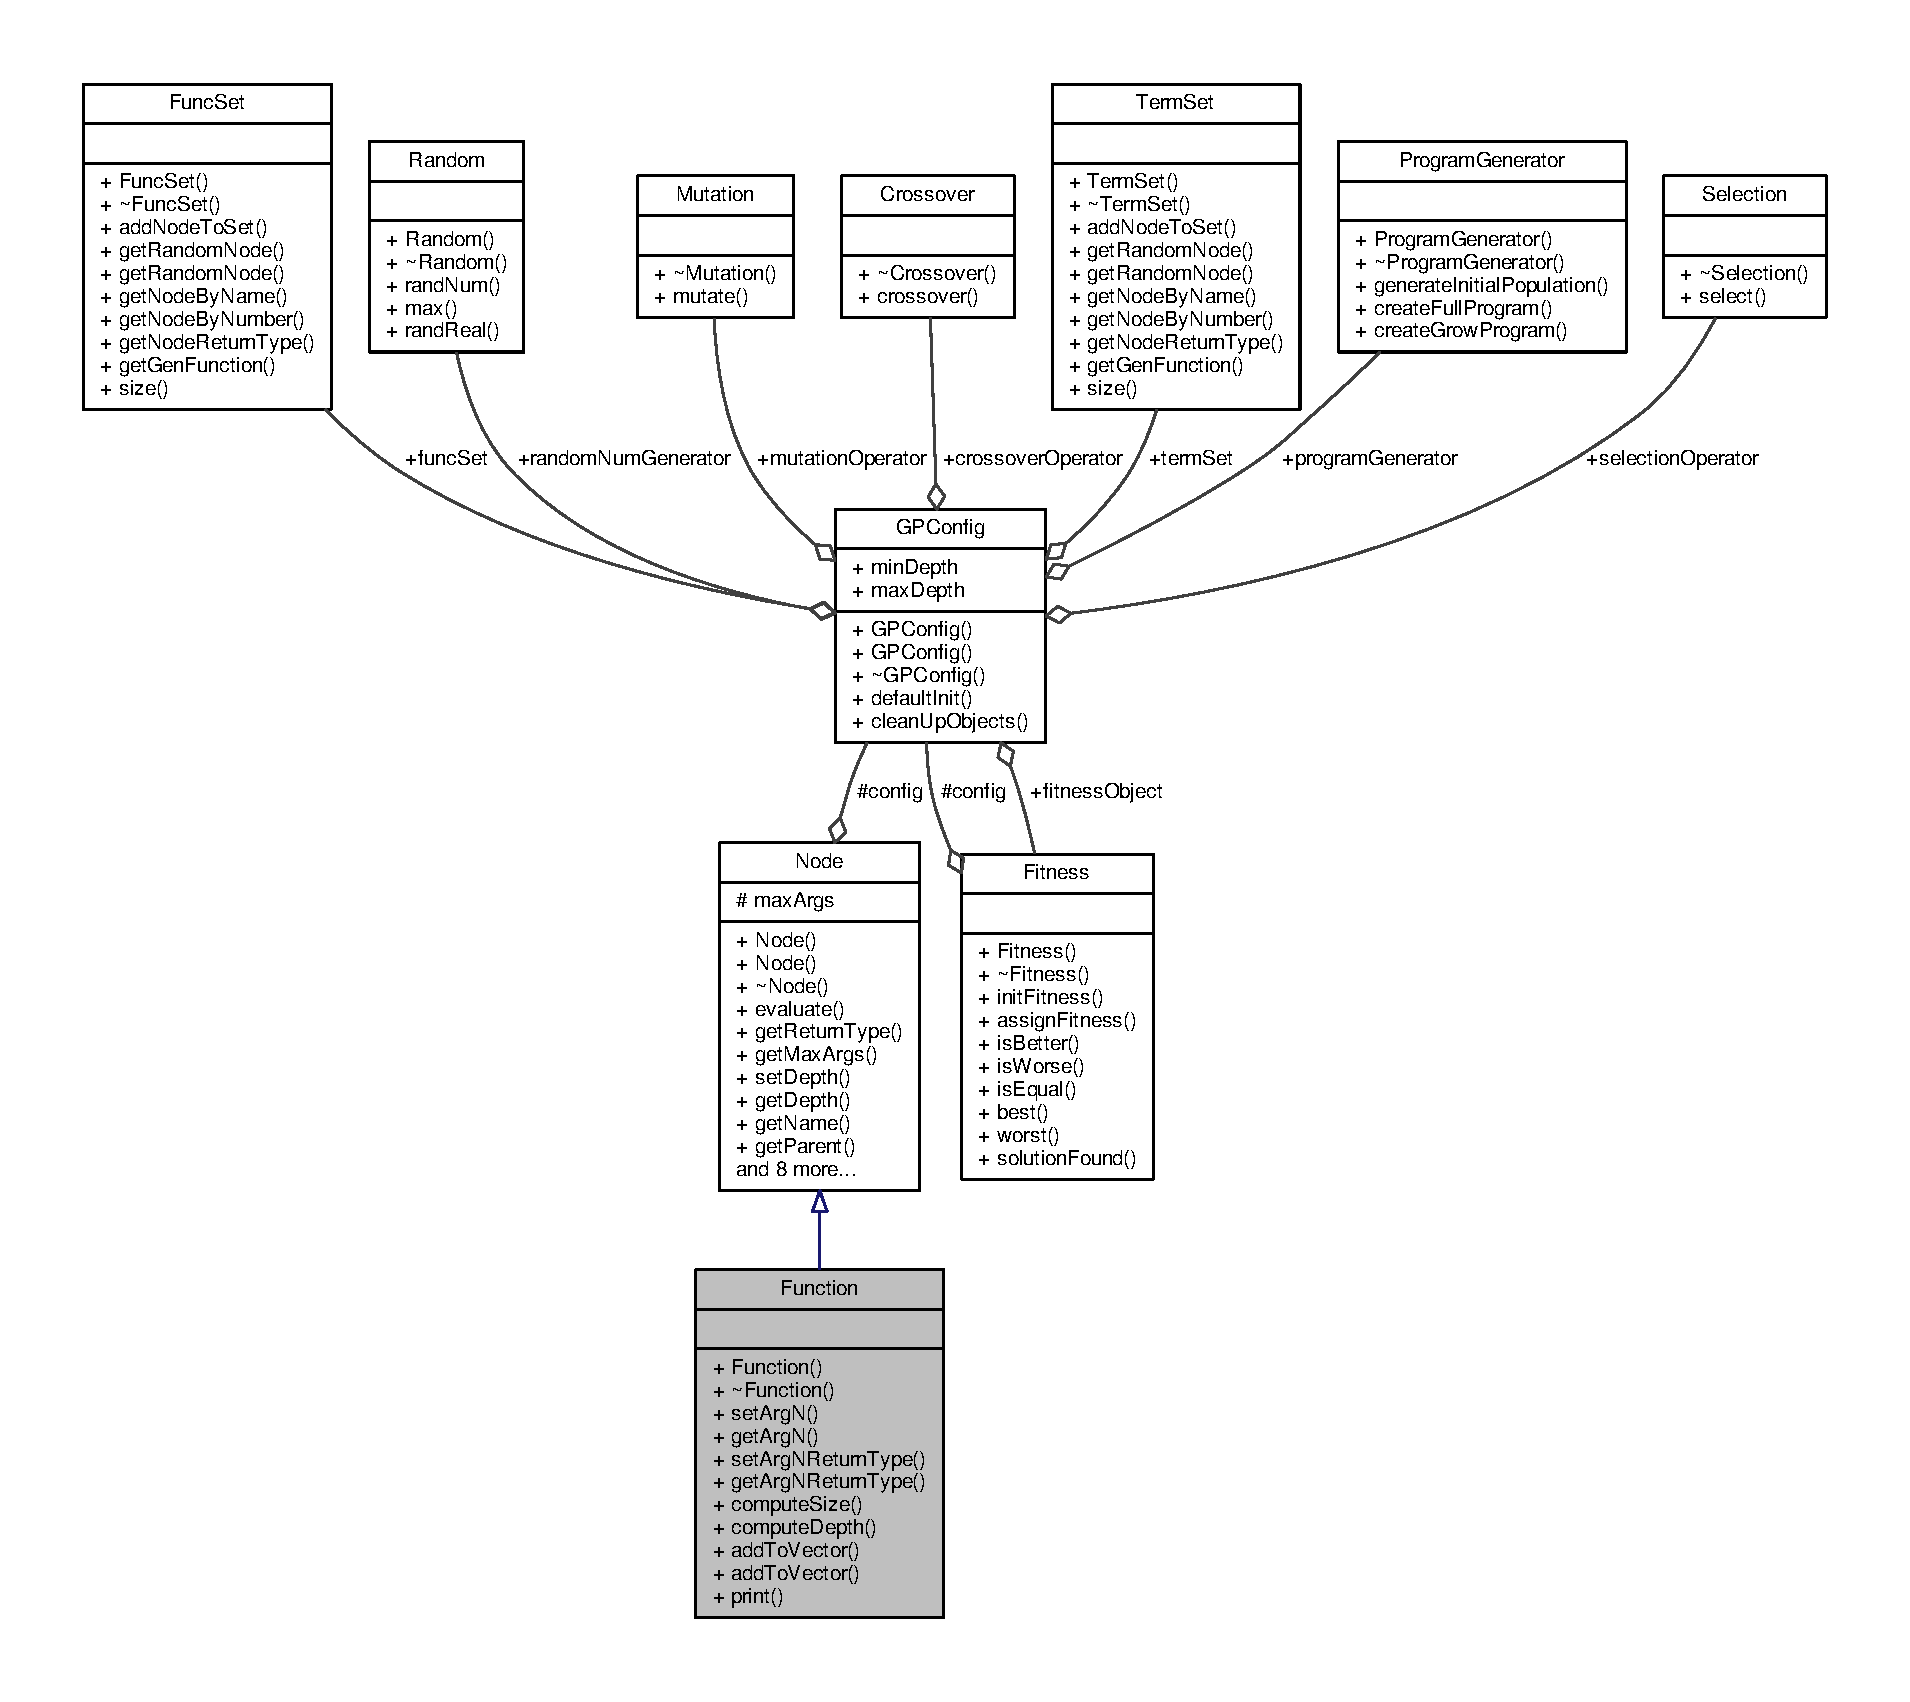
\includegraphics[width=350pt]{classFunction__coll__graph}
\end{center}
\end{figure}
\subsection*{Public Member Functions}
\begin{DoxyCompactItemize}
\item 
\hypertarget{classFunction_ac6ace12b3f85a5cc3cbac74d689a4c97}{}\label{classFunction_ac6ace12b3f85a5cc3cbac74d689a4c97} 
{\bfseries Function} (int type, int num\+Args, string n, \hyperlink{classGPConfig}{G\+P\+Config} $\ast$conf)
\item 
\hypertarget{classFunction_a8c700b4566ed38a2e0a2e43298006562}{}\label{classFunction_a8c700b4566ed38a2e0a2e43298006562} 
void {\bfseries set\+ArgN} (int N, \hyperlink{classNode}{Node} $\ast$n)
\item 
\hypertarget{classFunction_a7f59d12d6f9c025f624c8e7a3ba4ab50}{}\label{classFunction_a7f59d12d6f9c025f624c8e7a3ba4ab50} 
\hyperlink{classNode}{Node} $\ast$ {\bfseries get\+ArgN} (int N) const
\item 
\hypertarget{classFunction_a81f92fe00fb304d3843d921621b9ea92}{}\label{classFunction_a81f92fe00fb304d3843d921621b9ea92} 
void {\bfseries set\+Arg\+N\+Return\+Type} (int N, int type)
\item 
\hypertarget{classFunction_a806fff8d1517a3ef7e747bd680e8f1bc}{}\label{classFunction_a806fff8d1517a3ef7e747bd680e8f1bc} 
int {\bfseries get\+Arg\+N\+Return\+Type} (int N) const
\item 
\hypertarget{classFunction_aa4e87ae2aa129545e59c7fbefa6ff30b}{}\label{classFunction_aa4e87ae2aa129545e59c7fbefa6ff30b} 
virtual int {\bfseries compute\+Size} ()
\item 
\hypertarget{classFunction_a147422c1eaa324d692fb6edf35da3a59}{}\label{classFunction_a147422c1eaa324d692fb6edf35da3a59} 
virtual int {\bfseries compute\+Depth} (int cur\+Depth)
\item 
\hypertarget{classFunction_a426a42cef2b34a808a079bdcb53d8e54}{}\label{classFunction_a426a42cef2b34a808a079bdcb53d8e54} 
virtual void {\bfseries add\+To\+Vector} (vector$<$ \hyperlink{classNode}{Node} $\ast$$>$ \&vec)
\item 
\hypertarget{classFunction_a78671c12f81c0eb3e0a54a4df9716b94}{}\label{classFunction_a78671c12f81c0eb3e0a54a4df9716b94} 
virtual void {\bfseries add\+To\+Vector} (vector$<$ \hyperlink{classNode}{Node} $\ast$$>$ \&vec, int type\+Num)
\item 
\hypertarget{classFunction_a2d8cbf61ef2fb349958b818f87fedd83}{}\label{classFunction_a2d8cbf61ef2fb349958b818f87fedd83} 
virtual void {\bfseries print} (string \&s)
\end{DoxyCompactItemize}
\subsection*{Additional Inherited Members}


The documentation for this class was generated from the following files\+:\begin{DoxyCompactItemize}
\item 
/home/\+Lach/npr-\/v109/\+R\+M\+I\+T\+G\+P.\+1.\+5/Function.\+h\item 
/home/\+Lach/npr-\/v109/\+R\+M\+I\+T\+G\+P.\+1.\+5/Function.\+cpp\end{DoxyCompactItemize}

\hypertarget{classGeneticProgram}{}\section{Genetic\+Program Class Reference}
\label{classGeneticProgram}\index{Genetic\+Program@{Genetic\+Program}}


Collaboration diagram for Genetic\+Program\+:
\nopagebreak
\begin{figure}[H]
\begin{center}
\leavevmode
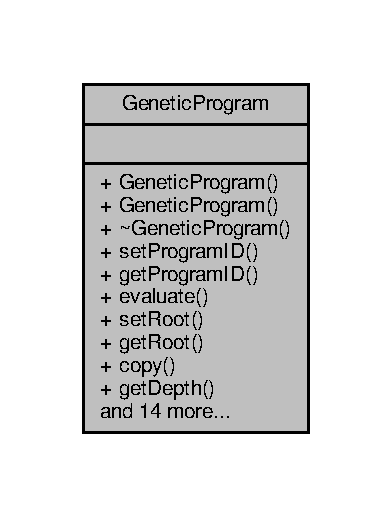
\includegraphics[width=188pt]{classGeneticProgram__coll__graph}
\end{center}
\end{figure}
\subsection*{Public Member Functions}
\begin{DoxyCompactItemize}
\item 
\hypertarget{classGeneticProgram_ab9e2508fa3c24361571569d09fc6a16c}{}\label{classGeneticProgram_ab9e2508fa3c24361571569d09fc6a16c} 
{\bfseries Genetic\+Program} (\hyperlink{classGPConfig}{G\+P\+Config} $\ast$conf)
\item 
\hypertarget{classGeneticProgram_aec99f476dfaaa2a2d63e0ae0b71bb31c}{}\label{classGeneticProgram_aec99f476dfaaa2a2d63e0ae0b71bb31c} 
{\bfseries Genetic\+Program} (\hyperlink{classGeneticProgram}{Genetic\+Program} \&g)
\item 
\hypertarget{classGeneticProgram_a8daa2e6454f2e38c4ee1879575ff60d1}{}\label{classGeneticProgram_a8daa2e6454f2e38c4ee1879575ff60d1} 
void {\bfseries set\+Program\+ID} (int id)
\item 
\hypertarget{classGeneticProgram_ac4270a77f69bbae79134e4e243be330a}{}\label{classGeneticProgram_ac4270a77f69bbae79134e4e243be330a} 
int {\bfseries get\+Program\+ID} () const
\item 
\hypertarget{classGeneticProgram_a2370fa2cacf7824f7ebadce840b0b2ea}{}\label{classGeneticProgram_a2370fa2cacf7824f7ebadce840b0b2ea} 
void {\bfseries evaluate} (\hyperlink{classReturnData}{Return\+Data} $\ast$out)
\item 
\hypertarget{classGeneticProgram_a60d27503bbf1b7a7e5d8590dfbc376f2}{}\label{classGeneticProgram_a60d27503bbf1b7a7e5d8590dfbc376f2} 
void {\bfseries set\+Root} (\hyperlink{classNode}{Node} $\ast$value)
\item 
\hypertarget{classGeneticProgram_a5ca5bd98689535360b4e8b282edceb83}{}\label{classGeneticProgram_a5ca5bd98689535360b4e8b282edceb83} 
\hyperlink{classNode}{Node} $\ast$ {\bfseries get\+Root} ()
\item 
\hypertarget{classGeneticProgram_ab46b8f5b1094253b9c86cfee676d88fe}{}\label{classGeneticProgram_ab46b8f5b1094253b9c86cfee676d88fe} 
\hyperlink{classGeneticProgram}{Genetic\+Program} $\ast$ {\bfseries copy} ()
\item 
\hypertarget{classGeneticProgram_a0236834ac9b8f4cd11703f9467c6d5b9}{}\label{classGeneticProgram_a0236834ac9b8f4cd11703f9467c6d5b9} 
int {\bfseries get\+Depth} () const
\item 
\hypertarget{classGeneticProgram_ae71d8e6193bec285f0821ce2b677804a}{}\label{classGeneticProgram_ae71d8e6193bec285f0821ce2b677804a} 
int {\bfseries get\+Size} () const
\item 
\hypertarget{classGeneticProgram_a7fcbcb1c72fb1123558d8c3458aa9630}{}\label{classGeneticProgram_a7fcbcb1c72fb1123558d8c3458aa9630} 
void {\bfseries compute\+Size\+And\+Depth} ()
\item 
\hypertarget{classGeneticProgram_a26d07af8f37418992cb031f748a6cd8e}{}\label{classGeneticProgram_a26d07af8f37418992cb031f748a6cd8e} 
\hyperlink{classNode}{Node} $\ast$ {\bfseries get\+Random\+Node} ()
\item 
\hypertarget{classGeneticProgram_a81c41b96e2d57f906558dfa7f8a557d9}{}\label{classGeneticProgram_a81c41b96e2d57f906558dfa7f8a557d9} 
\hyperlink{classNode}{Node} $\ast$ {\bfseries get\+Random\+Node} (int type\+Num)
\item 
\hypertarget{classGeneticProgram_a1532f6a6b458495c5dd399c74ea838e7}{}\label{classGeneticProgram_a1532f6a6b458495c5dd399c74ea838e7} 
void {\bfseries delete\+Tree} ()
\item 
\hypertarget{classGeneticProgram_ab11a81758b70a1a383598b3523712fe1}{}\label{classGeneticProgram_ab11a81758b70a1a383598b3523712fe1} 
void {\bfseries delete\+Tree} (\hyperlink{classNode}{Node} $\ast$the\+Root)
\item 
\hypertarget{classGeneticProgram_a18ac2cdc76a52cd7854af44008e0ba07}{}\label{classGeneticProgram_a18ac2cdc76a52cd7854af44008e0ba07} 
void {\bfseries print} (string \&s)
\item 
\hypertarget{classGeneticProgram_ac9e88c0250e07288e520c7e6b35b3d49}{}\label{classGeneticProgram_ac9e88c0250e07288e520c7e6b35b3d49} 
void {\bfseries set\+Return\+Type} (int type)
\item 
\hypertarget{classGeneticProgram_a962fb648e94aae61294e441da1674393}{}\label{classGeneticProgram_a962fb648e94aae61294e441da1674393} 
int {\bfseries get\+Return\+Type} () const
\item 
\hypertarget{classGeneticProgram_af8e4e08bf8c0eb2d1411bc91c1243b97}{}\label{classGeneticProgram_af8e4e08bf8c0eb2d1411bc91c1243b97} 
void {\bfseries set\+Fitness} (double f)
\item 
\hypertarget{classGeneticProgram_ab1c33e4a36a003d1154f1fae1c8899c6}{}\label{classGeneticProgram_ab1c33e4a36a003d1154f1fae1c8899c6} 
double {\bfseries get\+Fitness} () const
\item 
\hypertarget{classGeneticProgram_a7a6e3c1282b12e0da39331dc44c558ef}{}\label{classGeneticProgram_a7a6e3c1282b12e0da39331dc44c558ef} 
void {\bfseries set\+Adj\+Fitness} (double f)
\item 
\hypertarget{classGeneticProgram_a4051ef3b612dd063bb6287f787fb78fe}{}\label{classGeneticProgram_a4051ef3b612dd063bb6287f787fb78fe} 
double {\bfseries get\+Adj\+Fitness} () const
\item 
\hypertarget{classGeneticProgram_a1e482c80cf346bde1a5833614af3cd82}{}\label{classGeneticProgram_a1e482c80cf346bde1a5833614af3cd82} 
void {\bfseries parse\+Program} (string \&program\+String)
\end{DoxyCompactItemize}


The documentation for this class was generated from the following files\+:\begin{DoxyCompactItemize}
\item 
/home/\+Lach/npr-\/v109/\+R\+M\+I\+T\+G\+P.\+1.\+5/Genetic\+Program.\+h\item 
/home/\+Lach/npr-\/v109/\+R\+M\+I\+T\+G\+P.\+1.\+5/Genetic\+Program.\+cpp\end{DoxyCompactItemize}

\hypertarget{classGPConfig}{}\section{G\+P\+Config Class Reference}
\label{classGPConfig}\index{G\+P\+Config@{G\+P\+Config}}


Collaboration diagram for G\+P\+Config\+:
\nopagebreak
\begin{figure}[H]
\begin{center}
\leavevmode
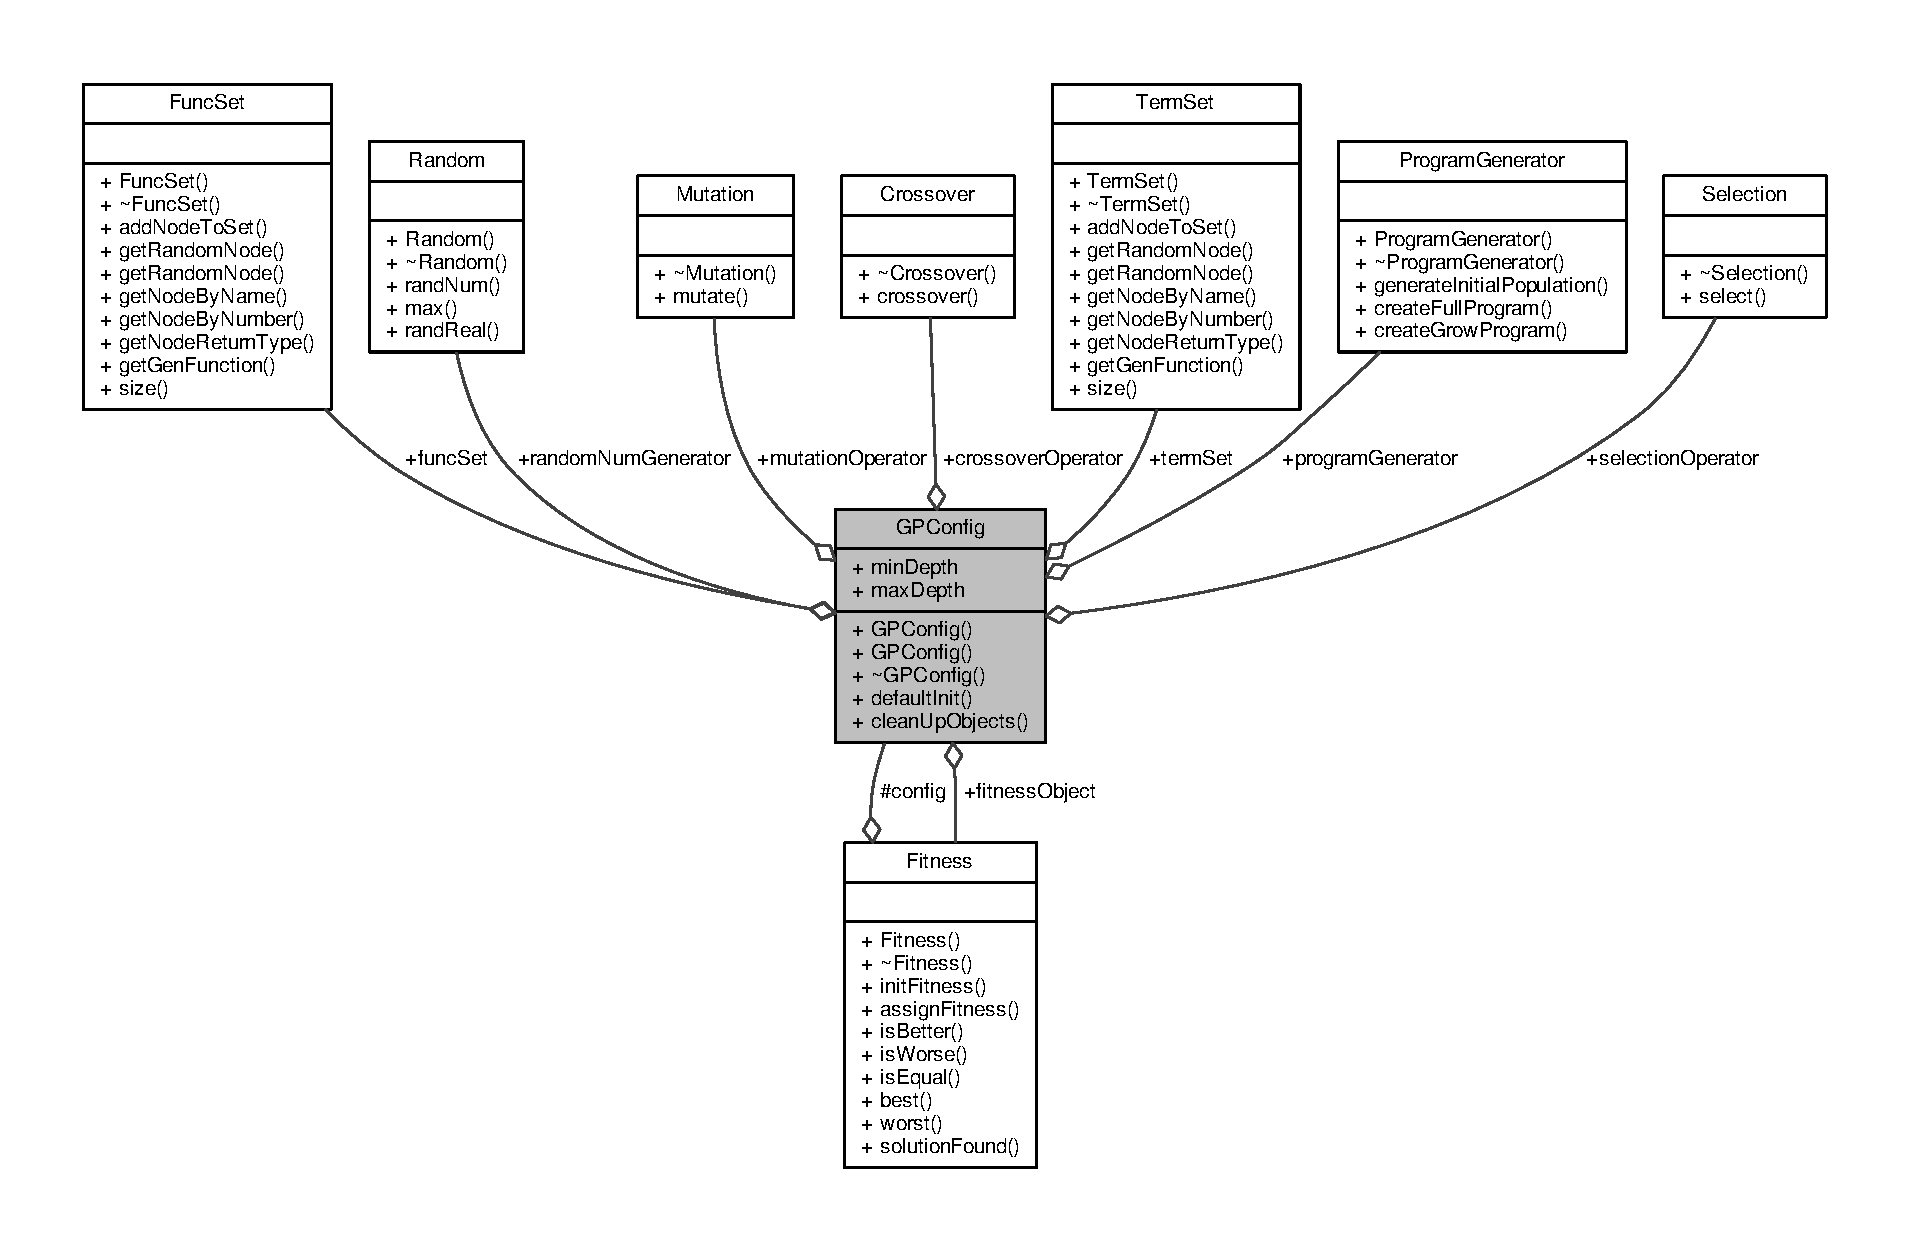
\includegraphics[width=350pt]{classGPConfig__coll__graph}
\end{center}
\end{figure}
\subsection*{Public Member Functions}
\begin{DoxyCompactItemize}
\item 
\hypertarget{classGPConfig_aab0af46c7d372c9a2f0586f02626c41d}{}\label{classGPConfig_aab0af46c7d372c9a2f0586f02626c41d} 
{\bfseries G\+P\+Config} (\hyperlink{classGPConfig}{G\+P\+Config} \&c)
\item 
\hypertarget{classGPConfig_a58149f4ce73c4551fabe5958b75aadee}{}\label{classGPConfig_a58149f4ce73c4551fabe5958b75aadee} 
virtual void {\bfseries default\+Init} ()
\item 
\hypertarget{classGPConfig_ac3031839d0721927269b57948d60c7b6}{}\label{classGPConfig_ac3031839d0721927269b57948d60c7b6} 
void {\bfseries clean\+Up\+Objects} ()
\end{DoxyCompactItemize}
\subsection*{Public Attributes}
\begin{DoxyCompactItemize}
\item 
\hypertarget{classGPConfig_a2f3cd90e27adbd9b268e5e971ea307a1}{}\label{classGPConfig_a2f3cd90e27adbd9b268e5e971ea307a1} 
int {\bfseries min\+Depth}
\item 
\hypertarget{classGPConfig_aa303ff5961d10678cf9a7450e86c865c}{}\label{classGPConfig_aa303ff5961d10678cf9a7450e86c865c} 
int {\bfseries max\+Depth}
\item 
\hypertarget{classGPConfig_a6e87e49e9df1a1099bd90841cc5007e4}{}\label{classGPConfig_a6e87e49e9df1a1099bd90841cc5007e4} 
\hyperlink{classFuncSet}{Func\+Set} {\bfseries func\+Set}
\item 
\hypertarget{classGPConfig_a0c61334e69d034e4dfa98c04703e7964}{}\label{classGPConfig_a0c61334e69d034e4dfa98c04703e7964} 
\hyperlink{classTermSet}{Term\+Set} {\bfseries term\+Set}
\item 
\hypertarget{classGPConfig_acf1e34811aefbf81986a0eb100fa05fd}{}\label{classGPConfig_acf1e34811aefbf81986a0eb100fa05fd} 
\hyperlink{classRandom}{Random} $\ast$ {\bfseries random\+Num\+Generator}
\item 
\hypertarget{classGPConfig_a29e9edd7b124a56391efc247ec0b5993}{}\label{classGPConfig_a29e9edd7b124a56391efc247ec0b5993} 
\hyperlink{classCrossover}{Crossover} $\ast$ {\bfseries crossover\+Operator}
\item 
\hypertarget{classGPConfig_a59f07ecbd6c5bef5747ff7b0d8df7d34}{}\label{classGPConfig_a59f07ecbd6c5bef5747ff7b0d8df7d34} 
\hyperlink{classMutation}{Mutation} $\ast$ {\bfseries mutation\+Operator}
\item 
\hypertarget{classGPConfig_a9c959060158716312a82be4a6ee4ed8f}{}\label{classGPConfig_a9c959060158716312a82be4a6ee4ed8f} 
\hyperlink{classSelection}{Selection} $\ast$ {\bfseries selection\+Operator}
\item 
\hypertarget{classGPConfig_a805803520f30f53973703b0c3cd56906}{}\label{classGPConfig_a805803520f30f53973703b0c3cd56906} 
\hyperlink{classFitness}{Fitness} $\ast$ {\bfseries fitness\+Object}
\item 
\hypertarget{classGPConfig_aad657d4dcb34731371624dc2f2ad04cb}{}\label{classGPConfig_aad657d4dcb34731371624dc2f2ad04cb} 
\hyperlink{classProgramGenerator}{Program\+Generator} $\ast$ {\bfseries program\+Generator}
\end{DoxyCompactItemize}


The documentation for this class was generated from the following files\+:\begin{DoxyCompactItemize}
\item 
/home/\+Lach/npr-\/v109/\+R\+M\+I\+T\+G\+P.\+1.\+5/G\+P\+Config.\+h\item 
/home/\+Lach/npr-\/v109/\+R\+M\+I\+T\+G\+P.\+1.\+5/G\+P\+Config.\+cpp\end{DoxyCompactItemize}

\hypertarget{classGridPopulation}{}\section{Grid\+Population Class Reference}
\label{classGridPopulation}\index{Grid\+Population@{Grid\+Population}}


Inheritance diagram for Grid\+Population\+:
\nopagebreak
\begin{figure}[H]
\begin{center}
\leavevmode
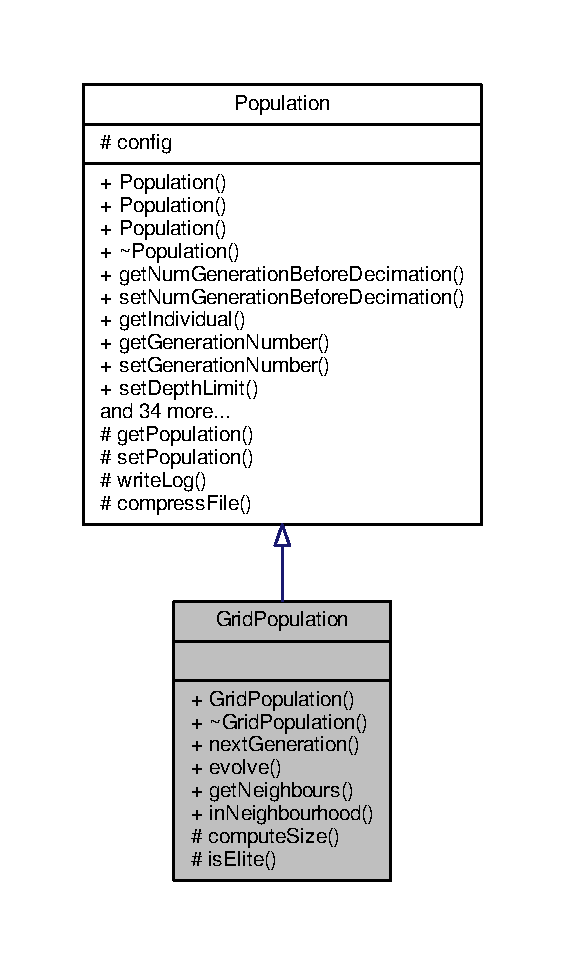
\includegraphics[width=271pt]{classGridPopulation__inherit__graph}
\end{center}
\end{figure}


Collaboration diagram for Grid\+Population\+:
\nopagebreak
\begin{figure}[H]
\begin{center}
\leavevmode
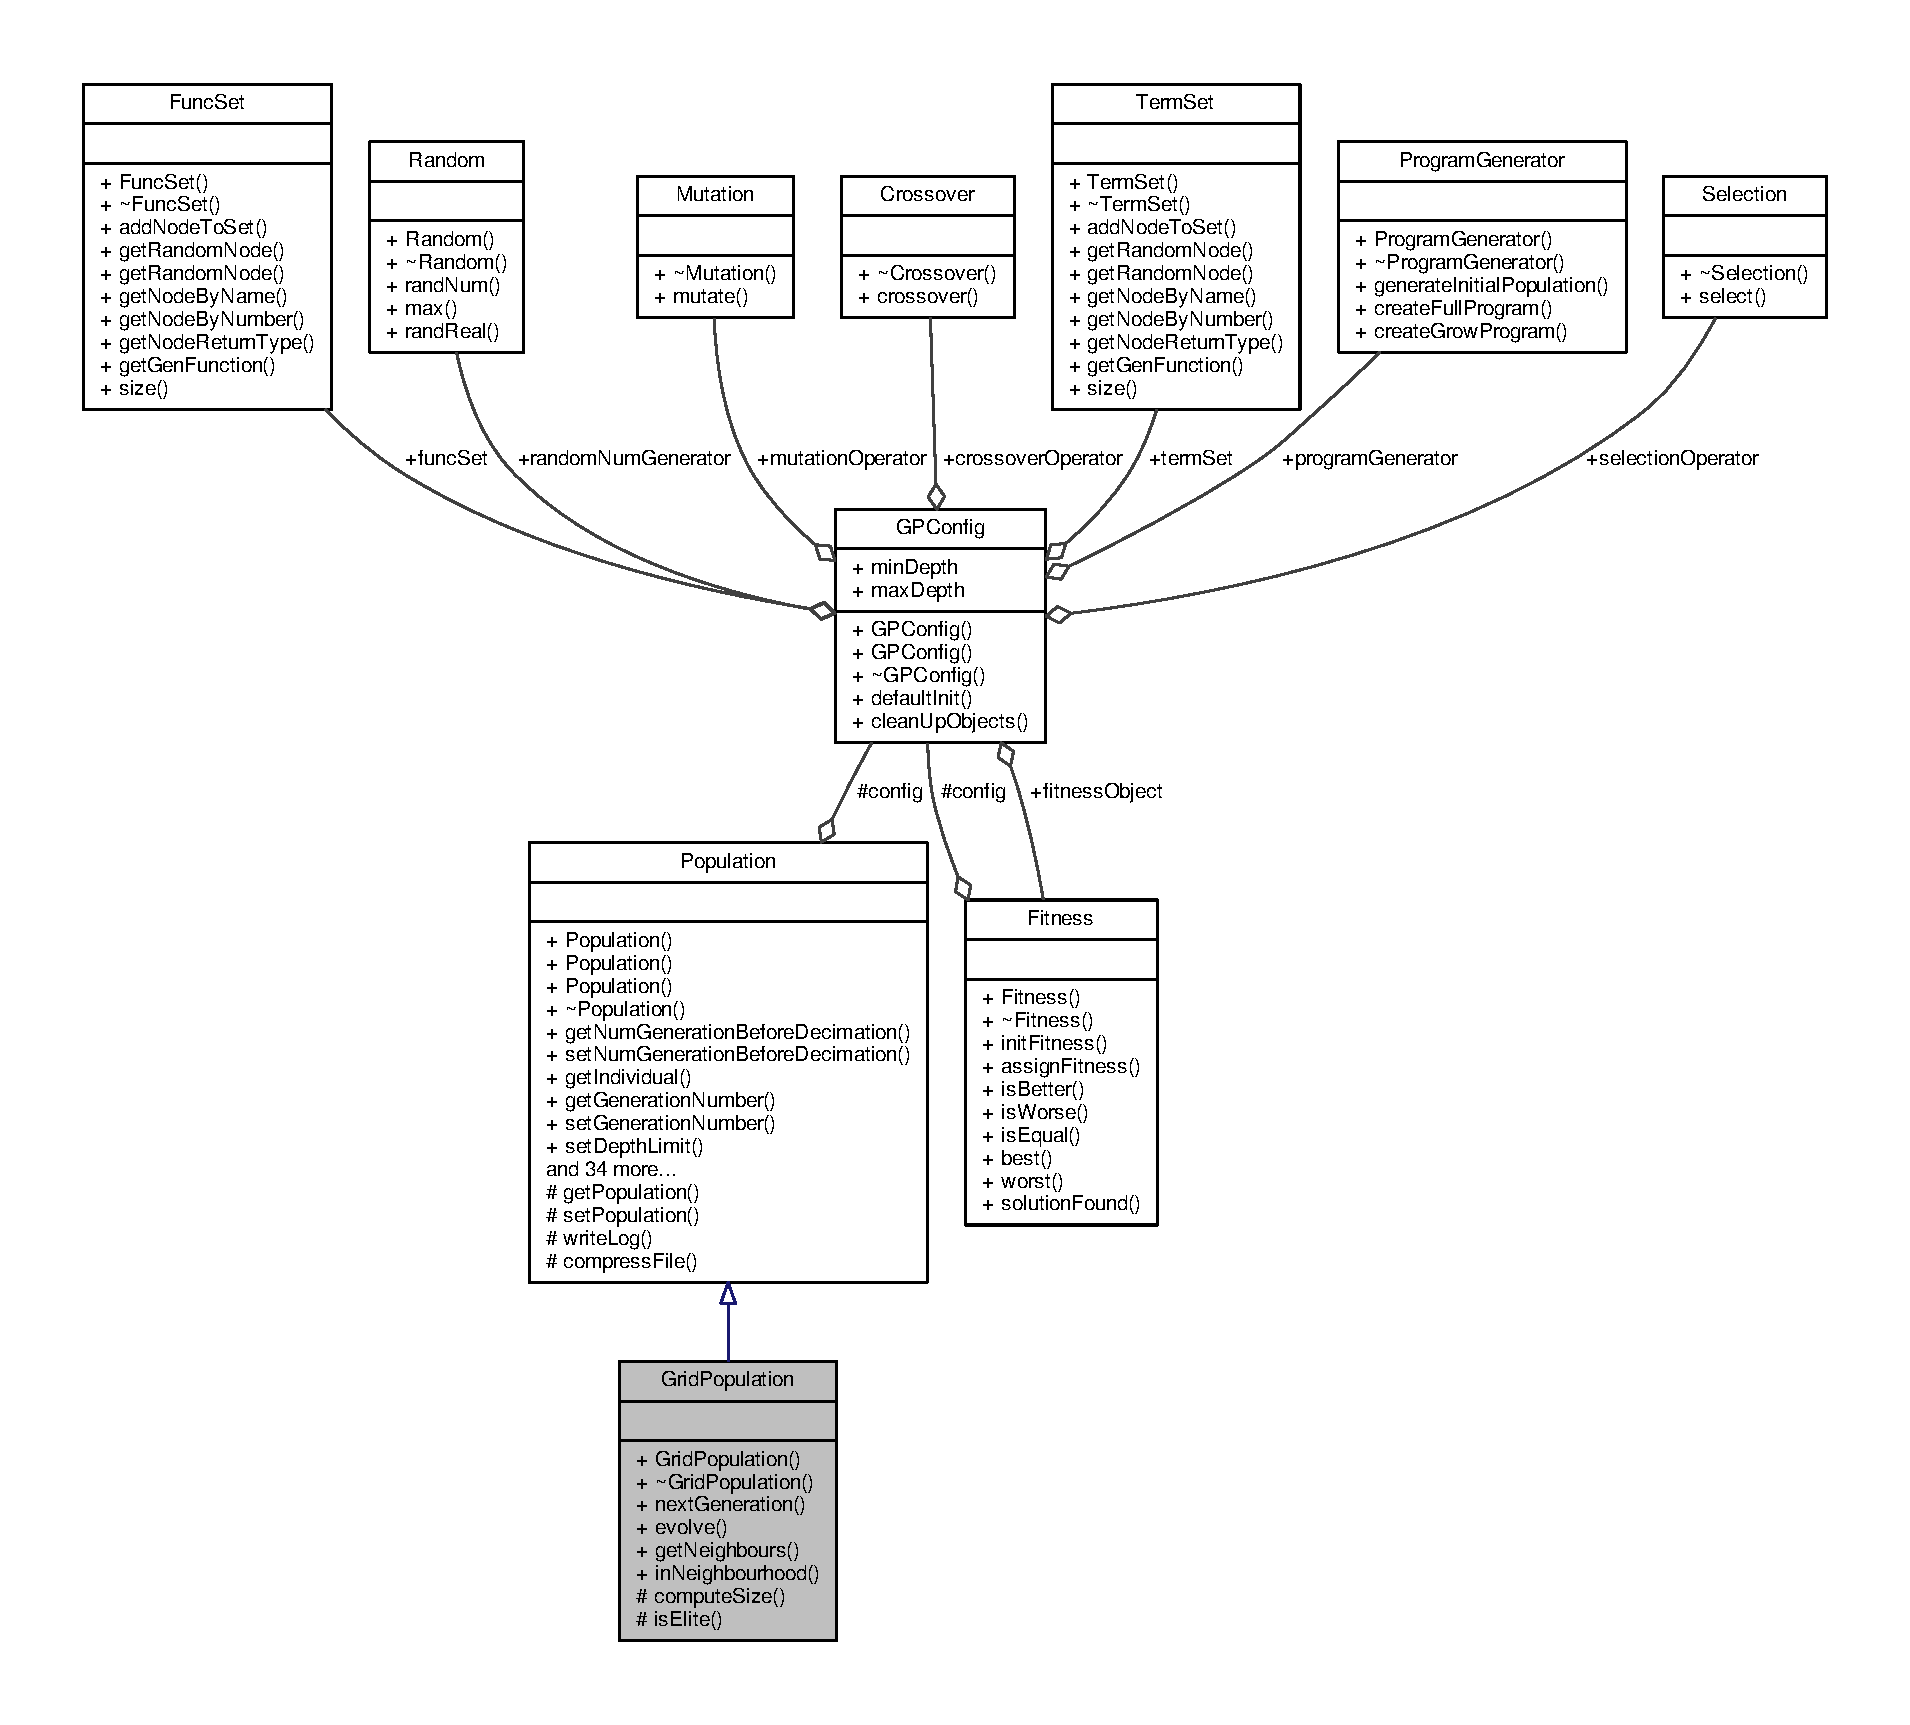
\includegraphics[width=350pt]{classGridPopulation__coll__graph}
\end{center}
\end{figure}
\subsection*{Public Member Functions}
\begin{DoxyCompactItemize}
\item 
\hypertarget{classGridPopulation_ad3529857b166c6e83969671d7dd1d1c9}{}\label{classGridPopulation_ad3529857b166c6e83969671d7dd1d1c9} 
{\bfseries Grid\+Population} (int x\+Size, int y\+Size, int dist, char $\ast$log\+File\+Name, \hyperlink{classGPConfig}{G\+P\+Config} $\ast$conf)
\item 
\hypertarget{classGridPopulation_a6e70ac22deef76063607ed924606b4be}{}\label{classGridPopulation_a6e70ac22deef76063607ed924606b4be} 
virtual void {\bfseries next\+Generation} ()
\item 
\hypertarget{classGridPopulation_a7d8b0eb0e9a22461322408032fef942f}{}\label{classGridPopulation_a7d8b0eb0e9a22461322408032fef942f} 
virtual bool {\bfseries evolve} (int num\+Generations)
\item 
\hypertarget{classGridPopulation_a5c6dc71b10a17a5f9bb574e86a21b6e5}{}\label{classGridPopulation_a5c6dc71b10a17a5f9bb574e86a21b6e5} 
virtual int {\bfseries get\+Neighbours} (int individual, int $\ast$numbers, \hyperlink{classGeneticProgram}{Genetic\+Program} $\ast$$\ast$dest)
\item 
\hypertarget{classGridPopulation_a3d6361d1c013d88f5e78186c017f8f20}{}\label{classGridPopulation_a3d6361d1c013d88f5e78186c017f8f20} 
virtual bool {\bfseries in\+Neighbourhood} (Point2D \&point, Point2D \&neighbour)
\end{DoxyCompactItemize}
\subsection*{Protected Member Functions}
\begin{DoxyCompactItemize}
\item 
\hypertarget{classGridPopulation_ab787bde0136b7fefc3eeabdf4f416676}{}\label{classGridPopulation_ab787bde0136b7fefc3eeabdf4f416676} 
virtual int {\bfseries compute\+Size} (int distance)
\item 
\hypertarget{classGridPopulation_a2a48584c03e41711526cd0825c6e0169}{}\label{classGridPopulation_a2a48584c03e41711526cd0825c6e0169} 
virtual bool {\bfseries is\+Elite} (\hyperlink{classGeneticProgram}{Genetic\+Program} $\ast$program, \hyperlink{classGeneticProgram}{Genetic\+Program} $\ast$$\ast$best, int num\+To\+Check)
\end{DoxyCompactItemize}
\subsection*{Additional Inherited Members}


The documentation for this class was generated from the following files\+:\begin{DoxyCompactItemize}
\item 
/home/\+Lach/npr-\/v109/\+R\+M\+I\+T\+G\+P.\+1.\+5/Grid\+Population.\+h\item 
/home/\+Lach/npr-\/v109/\+R\+M\+I\+T\+G\+P.\+1.\+5/Grid\+Population.\+cpp\end{DoxyCompactItemize}

\hypertarget{structHSV}{}\section{H\+SV Struct Reference}
\label{structHSV}\index{H\+SV@{H\+SV}}


Collaboration diagram for H\+SV\+:
\nopagebreak
\begin{figure}[H]
\begin{center}
\leavevmode
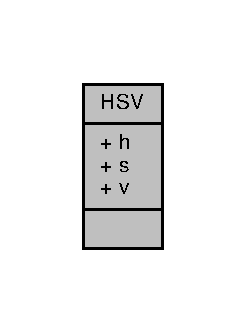
\includegraphics[width=118pt]{structHSV__coll__graph}
\end{center}
\end{figure}
\subsection*{Public Attributes}
\begin{DoxyCompactItemize}
\item 
\hypertarget{structHSV_ab038be2f08af85438d55554c5580d79c}{}\label{structHSV_ab038be2f08af85438d55554c5580d79c} 
int {\bfseries h}
\item 
\hypertarget{structHSV_a9bb3f6690e6879d417c4488b81cf90ca}{}\label{structHSV_a9bb3f6690e6879d417c4488b81cf90ca} 
int {\bfseries s}
\item 
\hypertarget{structHSV_acf84a724f9e1478f30f1238ca487ad69}{}\label{structHSV_acf84a724f9e1478f30f1238ca487ad69} 
int {\bfseries v}
\end{DoxyCompactItemize}


The documentation for this struct was generated from the following file\+:\begin{DoxyCompactItemize}
\item 
/home/\+Lach/npr-\/v109/src\+\_\+109/Utility.\+h\end{DoxyCompactItemize}

\hypertarget{classImageFitness}{}\section{Image\+Fitness Class Reference}
\label{classImageFitness}\index{Image\+Fitness@{Image\+Fitness}}


Inheritance diagram for Image\+Fitness\+:
\nopagebreak
\begin{figure}[H]
\begin{center}
\leavevmode
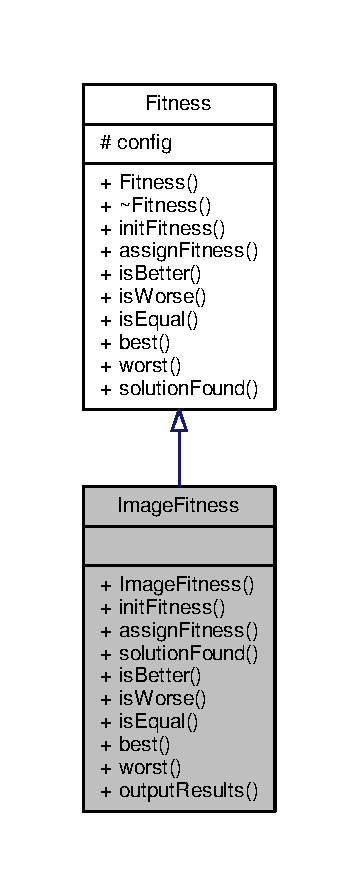
\includegraphics[width=172pt]{classImageFitness__inherit__graph}
\end{center}
\end{figure}


Collaboration diagram for Image\+Fitness\+:
\nopagebreak
\begin{figure}[H]
\begin{center}
\leavevmode
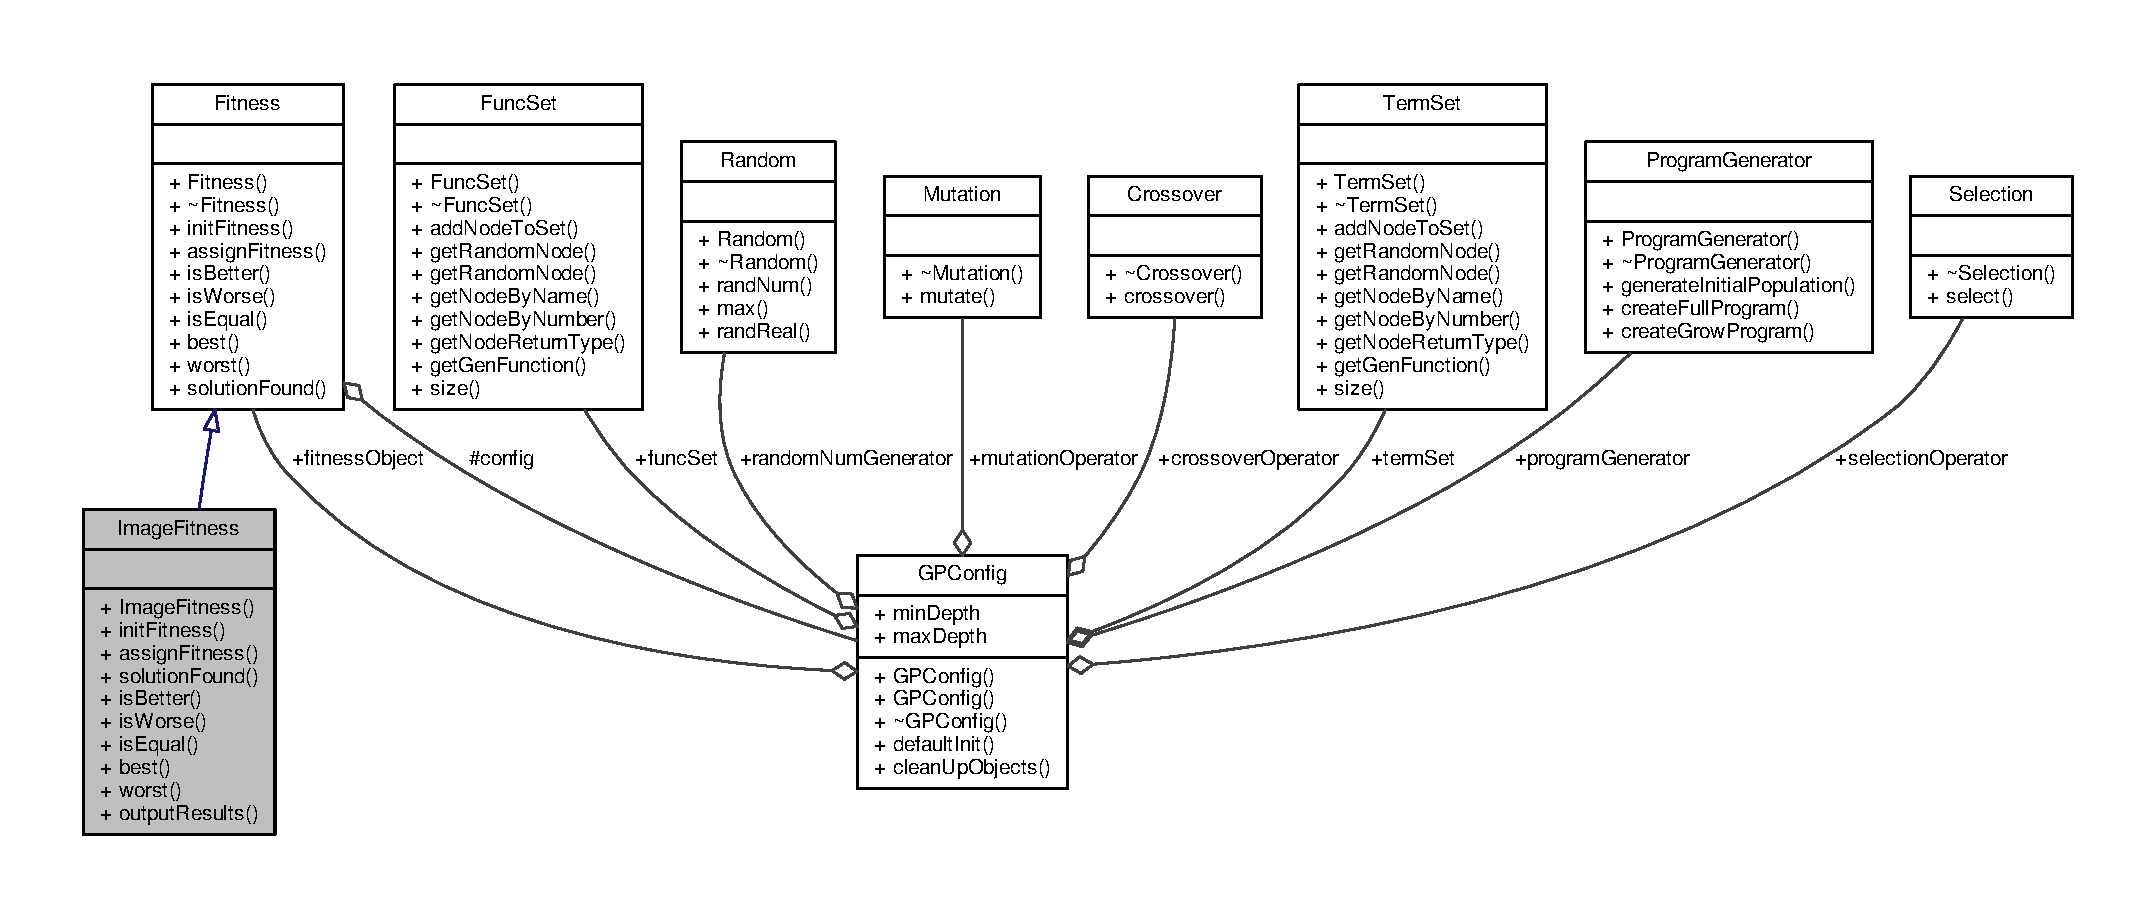
\includegraphics[width=350pt]{classImageFitness__coll__graph}
\end{center}
\end{figure}
\subsection*{Public Member Functions}
\begin{DoxyCompactItemize}
\item 
\hypertarget{classImageFitness_abe7707371984af9215fcd812b51defef}{}\label{classImageFitness_abe7707371984af9215fcd812b51defef} 
{\bfseries Image\+Fitness} (\hyperlink{classGPConfig}{G\+P\+Config} $\ast$conf)
\item 
\hypertarget{classImageFitness_a87b7ded1718e3a5ddf41855e18c060d3}{}\label{classImageFitness_a87b7ded1718e3a5ddf41855e18c060d3} 
virtual void {\bfseries init\+Fitness} ()
\item 
\hypertarget{classImageFitness_ab7a09b58e0f1aa28eb54e92b1c7c1e39}{}\label{classImageFitness_ab7a09b58e0f1aa28eb54e92b1c7c1e39} 
virtual void {\bfseries assign\+Fitness} (\hyperlink{classGeneticProgram}{Genetic\+Program} $\ast$pop\mbox{[}$\,$\mbox{]}, int pop\+Size)
\item 
\hypertarget{classImageFitness_a20dad1b0e981f8d0e6f968982566b073}{}\label{classImageFitness_a20dad1b0e981f8d0e6f968982566b073} 
virtual bool {\bfseries solution\+Found} (\hyperlink{classGeneticProgram}{Genetic\+Program} $\ast$pop\mbox{[}$\,$\mbox{]}, int pop\+Size)
\item 
\hypertarget{classImageFitness_a8b981e2d67357f1316bce965da2cb511}{}\label{classImageFitness_a8b981e2d67357f1316bce965da2cb511} 
virtual bool {\bfseries is\+Better} (\hyperlink{classGeneticProgram}{Genetic\+Program} $\ast$gp1, \hyperlink{classGeneticProgram}{Genetic\+Program} $\ast$gp2)
\item 
\hypertarget{classImageFitness_ad140d00e2dd89edc72ebceadf8aaee00}{}\label{classImageFitness_ad140d00e2dd89edc72ebceadf8aaee00} 
virtual bool {\bfseries is\+Worse} (\hyperlink{classGeneticProgram}{Genetic\+Program} $\ast$gp1, \hyperlink{classGeneticProgram}{Genetic\+Program} $\ast$gp2)
\item 
\hypertarget{classImageFitness_a49732d7c1838113c37dae1bf102643e9}{}\label{classImageFitness_a49732d7c1838113c37dae1bf102643e9} 
virtual bool {\bfseries is\+Equal} (\hyperlink{classGeneticProgram}{Genetic\+Program} $\ast$gp1, \hyperlink{classGeneticProgram}{Genetic\+Program} $\ast$gp2)
\item 
\hypertarget{classImageFitness_a7906f6594096f7ebaf5e64bcfb56a657}{}\label{classImageFitness_a7906f6594096f7ebaf5e64bcfb56a657} 
virtual double {\bfseries best} ()
\item 
\hypertarget{classImageFitness_a58acec0b8d5e84da69221aab18308c47}{}\label{classImageFitness_a58acec0b8d5e84da69221aab18308c47} 
virtual double {\bfseries worst} ()
\item 
\hypertarget{classImageFitness_a3834397e9a1486dc37b2e4eb133bc84f}{}\label{classImageFitness_a3834397e9a1486dc37b2e4eb133bc84f} 
void {\bfseries output\+Results} (\hyperlink{classGeneticProgram}{Genetic\+Program} $\ast$, char $\ast$, char $\ast$, double)
\end{DoxyCompactItemize}
\subsection*{Additional Inherited Members}


The documentation for this class was generated from the following files\+:\begin{DoxyCompactItemize}
\item 
/home/\+Lach/npr-\/v109/src\+\_\+109/Image\+Fitness.\+h\item 
/home/\+Lach/npr-\/v109/src\+\_\+109/Image\+Fitness.\+cpp\end{DoxyCompactItemize}

\hypertarget{classMaskMaker}{}\section{Mask\+Maker Class Reference}
\label{classMaskMaker}\index{Mask\+Maker@{Mask\+Maker}}


Collaboration diagram for Mask\+Maker\+:
\nopagebreak
\begin{figure}[H]
\begin{center}
\leavevmode
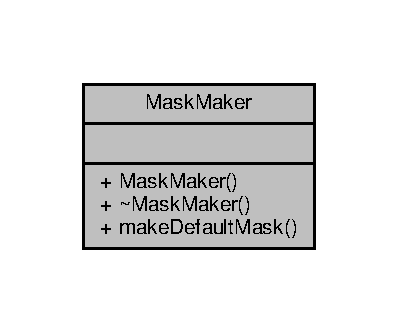
\includegraphics[width=191pt]{classMaskMaker__coll__graph}
\end{center}
\end{figure}
\subsection*{Public Member Functions}
\begin{DoxyCompactItemize}
\item 
\hypertarget{classMaskMaker_a94e5e9132a4dd3e4e1d8d1cdc8e0fcd2}{}\label{classMaskMaker_a94e5e9132a4dd3e4e1d8d1cdc8e0fcd2} 
{\bfseries Mask\+Maker} (const char $\ast$source\+File, const char $\ast$output\+File, unsigned T, unsigned N)
\item 
\hypertarget{classMaskMaker_a0fe6264b064fa722664f2eefb73af9e1}{}\label{classMaskMaker_a0fe6264b064fa722664f2eefb73af9e1} 
void {\bfseries make\+Default\+Mask} ()
\end{DoxyCompactItemize}


The documentation for this class was generated from the following files\+:\begin{DoxyCompactItemize}
\item 
/home/\+Lach/npr-\/v109/src\+\_\+109/Mask\+Maker.\+h\item 
/home/\+Lach/npr-\/v109/src\+\_\+109/Mask\+Maker.\+cpp\end{DoxyCompactItemize}

\hypertarget{classMutation}{}\section{Mutation Class Reference}
\label{classMutation}\index{Mutation@{Mutation}}


Collaboration diagram for Mutation\+:
\nopagebreak
\begin{figure}[H]
\begin{center}
\leavevmode
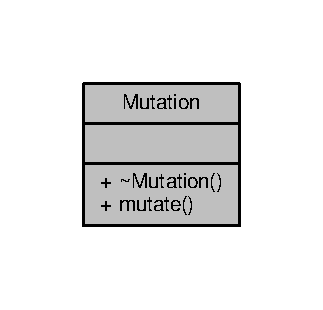
\includegraphics[width=155pt]{classMutation__coll__graph}
\end{center}
\end{figure}
\subsection*{Public Member Functions}
\begin{DoxyCompactItemize}
\item 
\hypertarget{classMutation_a49ce75b387f10483d51ef12af9525f1a}{}\label{classMutation_a49ce75b387f10483d51ef12af9525f1a} 
virtual void {\bfseries mutate} (\hyperlink{classGeneticProgram}{Genetic\+Program} \&gp, \hyperlink{classGPConfig}{G\+P\+Config} $\ast$conf)
\end{DoxyCompactItemize}


The documentation for this class was generated from the following files\+:\begin{DoxyCompactItemize}
\item 
/home/\+Lach/npr-\/v109/\+R\+M\+I\+T\+G\+P.\+1.\+5/Mutation.\+h\item 
/home/\+Lach/npr-\/v109/\+R\+M\+I\+T\+G\+P.\+1.\+5/Mutation.\+cpp\end{DoxyCompactItemize}

\hypertarget{classNode}{}\section{Node Class Reference}
\label{classNode}\index{Node@{Node}}


Inheritance diagram for Node\+:
\nopagebreak
\begin{figure}[H]
\begin{center}
\leavevmode
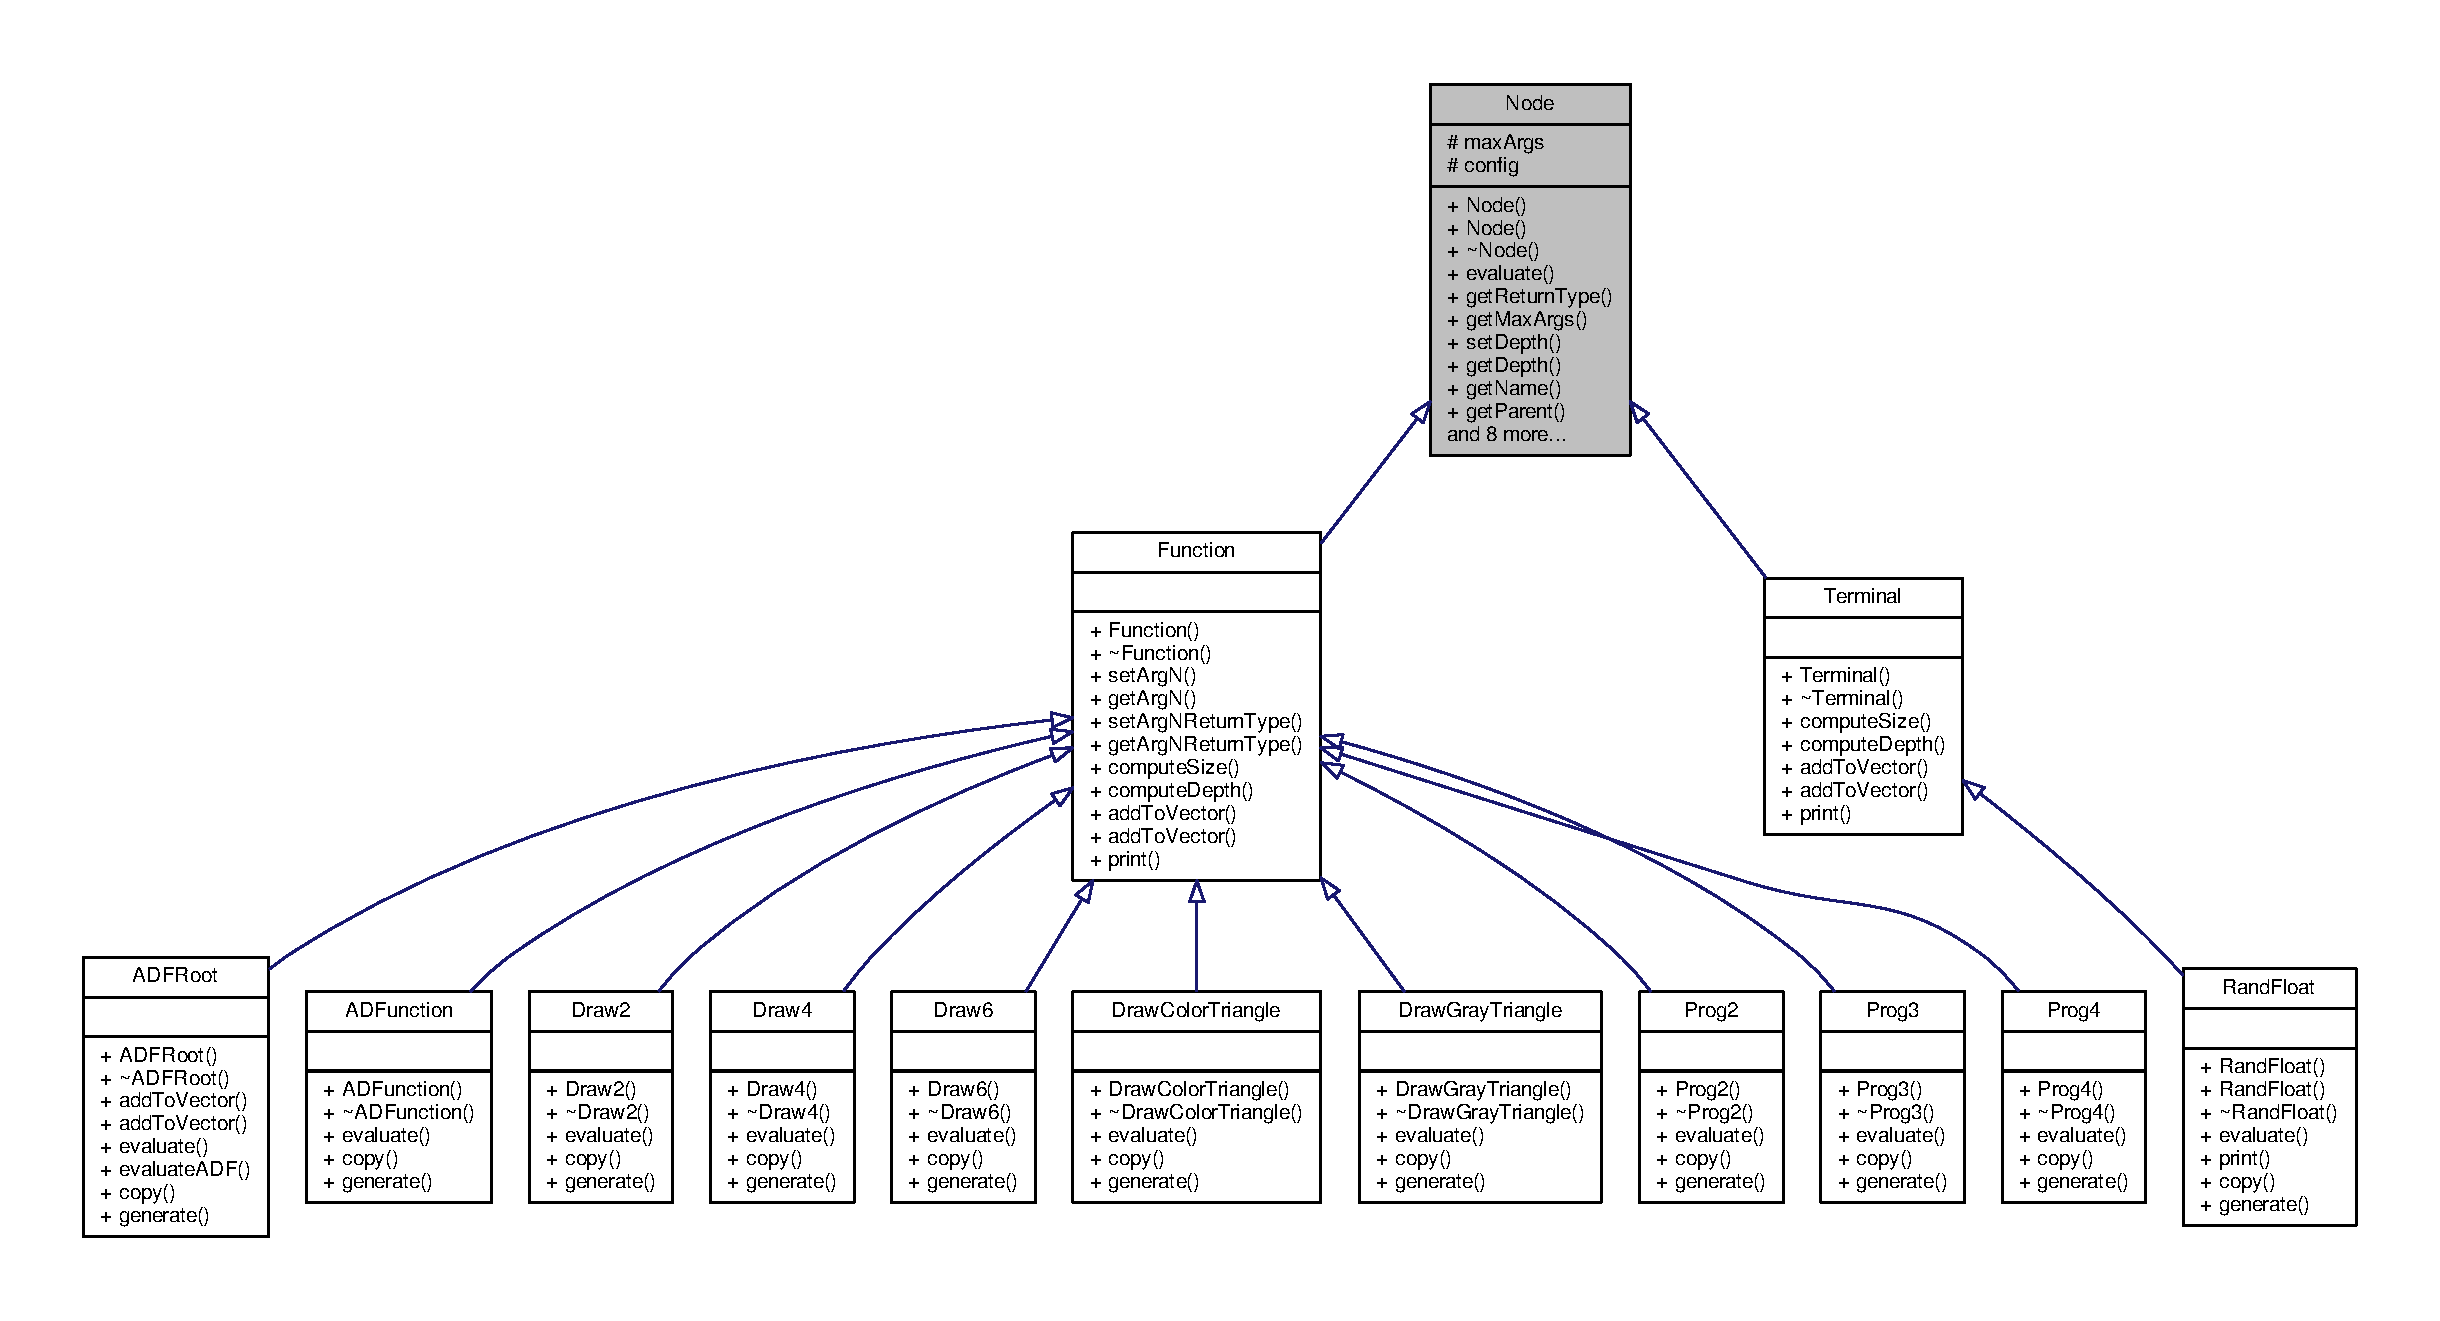
\includegraphics[width=350pt]{classNode__inherit__graph}
\end{center}
\end{figure}


Collaboration diagram for Node\+:
\nopagebreak
\begin{figure}[H]
\begin{center}
\leavevmode
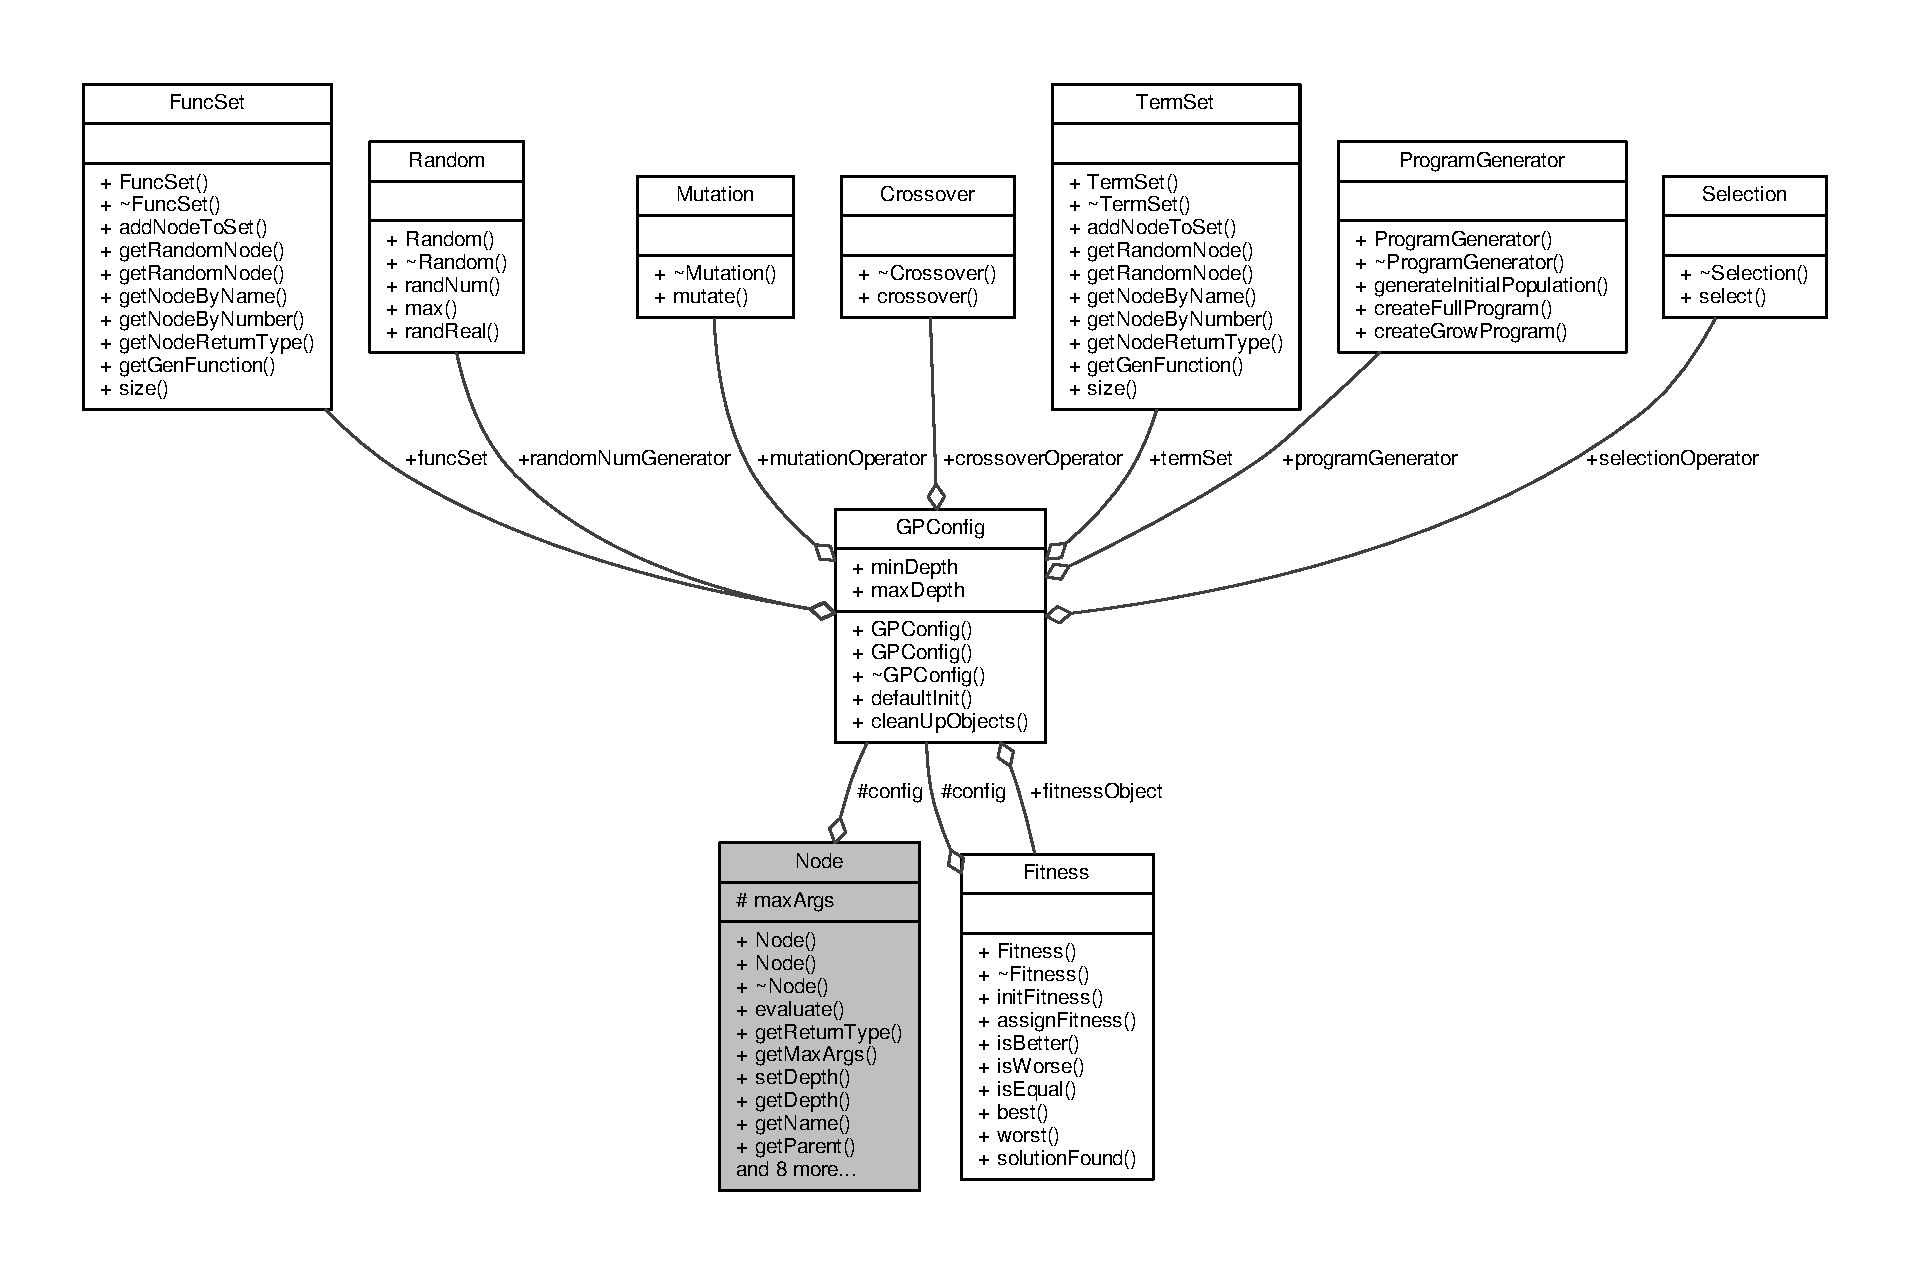
\includegraphics[width=350pt]{classNode__coll__graph}
\end{center}
\end{figure}
\subsection*{Public Member Functions}
\begin{DoxyCompactItemize}
\item 
\hypertarget{classNode_ae883e3232f71ca37b0523927bf57a7b6}{}\label{classNode_ae883e3232f71ca37b0523927bf57a7b6} 
{\bfseries Node} (int type, int num\+Args, string name, \hyperlink{classGPConfig}{G\+P\+Config} $\ast$conf)
\item 
\hypertarget{classNode_a8264fbb54d07be499bdc93e785f79351}{}\label{classNode_a8264fbb54d07be499bdc93e785f79351} 
{\bfseries Node} (\hyperlink{classNode}{Node} \&n)
\item 
\hypertarget{classNode_aa03774d17d9f331d7fc65c604bd04bc5}{}\label{classNode_aa03774d17d9f331d7fc65c604bd04bc5} 
virtual void {\bfseries evaluate} (\hyperlink{classReturnData}{Return\+Data} $\ast$out)=0
\item 
\hypertarget{classNode_a3bc9da611ff37236175a80c71e9eb350}{}\label{classNode_a3bc9da611ff37236175a80c71e9eb350} 
int {\bfseries get\+Return\+Type} () const
\item 
\hypertarget{classNode_afe50ea7da284533d08ab1c3965b32620}{}\label{classNode_afe50ea7da284533d08ab1c3965b32620} 
int {\bfseries get\+Max\+Args} () const
\item 
\hypertarget{classNode_a6c55a155ccbbcd8d62fb7300c5354715}{}\label{classNode_a6c55a155ccbbcd8d62fb7300c5354715} 
void {\bfseries set\+Depth} (const int d)
\item 
\hypertarget{classNode_a5cf0aef99d92c05310e12966273a0e7c}{}\label{classNode_a5cf0aef99d92c05310e12966273a0e7c} 
int {\bfseries get\+Depth} () const
\item 
\hypertarget{classNode_a33b290707977cb91f336bd7a40a6bd3a}{}\label{classNode_a33b290707977cb91f336bd7a40a6bd3a} 
string {\bfseries get\+Name} () const
\item 
\hypertarget{classNode_a3cad655320d50751c43c5cec9356dcf3}{}\label{classNode_a3cad655320d50751c43c5cec9356dcf3} 
\hyperlink{classNode}{Node} $\ast$ {\bfseries get\+Parent} () const
\item 
\hypertarget{classNode_a7aa7ebe6ad965b1ed545e8b12d823c1d}{}\label{classNode_a7aa7ebe6ad965b1ed545e8b12d823c1d} 
\hyperlink{classNode}{Node} $\ast$ {\bfseries get\+Root\+Node} () const
\item 
\hypertarget{classNode_ad7c28414b0d242ce7c491e22cf006041}{}\label{classNode_ad7c28414b0d242ce7c491e22cf006041} 
void {\bfseries set\+Parent} (\hyperlink{classNode}{Node} $\ast$n)
\item 
\hypertarget{classNode_a465c78ca0653d656c4b6be729a01e619}{}\label{classNode_a465c78ca0653d656c4b6be729a01e619} 
virtual int {\bfseries compute\+Size} ()=0
\item 
\hypertarget{classNode_a736c8c6ff2675222fffb054c8b5e71cf}{}\label{classNode_a736c8c6ff2675222fffb054c8b5e71cf} 
virtual int {\bfseries compute\+Depth} (int cur\+Depth)=0
\item 
\hypertarget{classNode_ae18241c6519adc9a20d2187a46c0dc6e}{}\label{classNode_ae18241c6519adc9a20d2187a46c0dc6e} 
virtual void {\bfseries add\+To\+Vector} (vector$<$ \hyperlink{classNode}{Node} $\ast$$>$ \&vec)=0
\item 
\hypertarget{classNode_a2c1e22a28cacaf7a1033377574b4ed23}{}\label{classNode_a2c1e22a28cacaf7a1033377574b4ed23} 
virtual void {\bfseries add\+To\+Vector} (vector$<$ \hyperlink{classNode}{Node} $\ast$$>$ \&vec, int type\+Num)=0
\item 
\hypertarget{classNode_a62fe30e16e81b24c73cf93b1577de5c0}{}\label{classNode_a62fe30e16e81b24c73cf93b1577de5c0} 
virtual void {\bfseries print} (string \&s)=0
\item 
\hypertarget{classNode_a3f9b0b2b5678e23f143c9fdaaf3e8c5c}{}\label{classNode_a3f9b0b2b5678e23f143c9fdaaf3e8c5c} 
virtual \hyperlink{classNode}{Node} $\ast$ {\bfseries copy} ()=0
\end{DoxyCompactItemize}
\subsection*{Protected Attributes}
\begin{DoxyCompactItemize}
\item 
\hypertarget{classNode_afc05e3b5c6bf0eace3fd8d8df8a15c7c}{}\label{classNode_afc05e3b5c6bf0eace3fd8d8df8a15c7c} 
int {\bfseries max\+Args}
\item 
\hypertarget{classNode_ae0353541456b3dcd4ed5521cbe7215fc}{}\label{classNode_ae0353541456b3dcd4ed5521cbe7215fc} 
\hyperlink{classGPConfig}{G\+P\+Config} $\ast$ {\bfseries config}
\end{DoxyCompactItemize}


The documentation for this class was generated from the following files\+:\begin{DoxyCompactItemize}
\item 
/home/\+Lach/npr-\/v109/\+R\+M\+I\+T\+G\+P.\+1.\+5/Node.\+h\item 
/home/\+Lach/npr-\/v109/\+R\+M\+I\+T\+G\+P.\+1.\+5/Node.\+cpp\end{DoxyCompactItemize}

\hypertarget{classNodeVector}{}\section{Node\+Vector$<$ Type $>$ Class Template Reference}
\label{classNodeVector}\index{Node\+Vector$<$ Type $>$@{Node\+Vector$<$ Type $>$}}


Collaboration diagram for Node\+Vector$<$ Type $>$\+:
\nopagebreak
\begin{figure}[H]
\begin{center}
\leavevmode
\includegraphics[width=225pt]{classNodeVector__coll__graph}
\end{center}
\end{figure}
\subsection*{Classes}
\begin{DoxyCompactItemize}
\item 
class \hyperlink{classNodeVector_1_1Element}{Element}
\end{DoxyCompactItemize}
\subsection*{Public Member Functions}
\begin{DoxyCompactItemize}
\item 
\hypertarget{classNodeVector_a38cd6775097581eb3fa51904505551ca}{}\label{classNodeVector_a38cd6775097581eb3fa51904505551ca} 
virtual void {\bfseries set\+G\+P\+Config} (\hyperlink{classGPConfig}{G\+P\+Config} $\ast$conf)
\item 
\hypertarget{classNodeVector_a35b8d230582dc5f2fca7005ed1f56277}{}\label{classNodeVector_a35b8d230582dc5f2fca7005ed1f56277} 
virtual void {\bfseries add\+Element} (\hyperlink{classNodeVector_1_1Element}{Element} elem)
\item 
\hypertarget{classNodeVector_a5bfc55e64d49c06d1ecad86d0f5cd5fb}{}\label{classNodeVector_a5bfc55e64d49c06d1ecad86d0f5cd5fb} 
virtual \hyperlink{classNodeVector_1_1Element}{Element} $\ast$ {\bfseries get\+Element} (int pos)
\item 
\hypertarget{classNodeVector_aa9d5b553e48aed8fd27404a646622a93}{}\label{classNodeVector_aa9d5b553e48aed8fd27404a646622a93} 
virtual Type $\ast$ {\bfseries get\+Random\+Element} ()
\item 
\hypertarget{classNodeVector_a6654cfbddb5867db262f388447ea7596}{}\label{classNodeVector_a6654cfbddb5867db262f388447ea7596} 
virtual Type $\ast$ {\bfseries get\+Random\+Typed\+Element} (int return\+Type)
\item 
\hypertarget{classNodeVector_a216c2a874bacd4f5c351ee4875c13a32}{}\label{classNodeVector_a216c2a874bacd4f5c351ee4875c13a32} 
virtual int {\bfseries size} () const
\end{DoxyCompactItemize}


The documentation for this class was generated from the following files\+:\begin{DoxyCompactItemize}
\item 
/home/\+Lach/npr-\/v109/\+R\+M\+I\+T\+G\+P.\+1.\+5/Node\+Set.\+h\item 
/home/\+Lach/npr-\/v109/\+R\+M\+I\+T\+G\+P.\+1.\+5/Node\+Vector.\+h\end{DoxyCompactItemize}

\hypertarget{classPalette}{}\section{Palette Class Reference}
\label{classPalette}\index{Palette@{Palette}}


Collaboration diagram for Palette\+:
\nopagebreak
\begin{figure}[H]
\begin{center}
\leavevmode
\includegraphics[width=194pt]{classPalette__coll__graph}
\end{center}
\end{figure}
\subsection*{Public Member Functions}
\begin{DoxyCompactItemize}
\item 
\hypertarget{classPalette_a9e7d1cfc83132e54f881c95acf0cb0d9}{}\label{classPalette_a9e7d1cfc83132e54f881c95acf0cb0d9} 
{\bfseries Palette} (\hyperlink{classTarget}{Target} $\ast$target)
\item 
\hypertarget{classPalette_ab861218bb6b4b64f24c774deaf26cada}{}\label{classPalette_ab861218bb6b4b64f24c774deaf26cada} 
{\bfseries Palette} (const char $\ast$)
\item 
\hypertarget{classPalette_abec7160109e458ab445ba1eaf752ab85}{}\label{classPalette_abec7160109e458ab445ba1eaf752ab85} 
\hyperlink{structRGB}{R\+GB} {\bfseries get\+Random\+R\+GB} (float f)
\item 
\hypertarget{classPalette_a11248e33e13b761d483f251ec21d9d11}{}\label{classPalette_a11248e33e13b761d483f251ec21d9d11} 
\hyperlink{structHSV}{H\+SV} {\bfseries get\+Random\+H\+SV} (float f)
\item 
\hypertarget{classPalette_a016d36d5c8d07f336291dd06841e7569}{}\label{classPalette_a016d36d5c8d07f336291dd06841e7569} 
\hyperlink{structRGB}{R\+GB} {\bfseries make\+Random\+R\+GB} ()
\item 
\hypertarget{classPalette_a1f6bd00bd930ba9ca75327871adedcb5}{}\label{classPalette_a1f6bd00bd930ba9ca75327871adedcb5} 
\hyperlink{structHSV}{H\+SV} {\bfseries make\+Random\+H\+SV} ()
\end{DoxyCompactItemize}


The documentation for this class was generated from the following files\+:\begin{DoxyCompactItemize}
\item 
/home/\+Lach/npr-\/v109/src\+\_\+109/Palette.\+h\item 
/home/\+Lach/npr-\/v109/src\+\_\+109/Palette.\+cpp\end{DoxyCompactItemize}

\hypertarget{classPixel}{}\section{Pixel Class Reference}
\label{classPixel}\index{Pixel@{Pixel}}


Collaboration diagram for Pixel\+:
\nopagebreak
\begin{figure}[H]
\begin{center}
\leavevmode
\includegraphics[width=160pt]{classPixel__coll__graph}
\end{center}
\end{figure}
\subsection*{Public Member Functions}
\begin{DoxyCompactItemize}
\item 
\hypertarget{classPixel_afe2eb7843df8e519d6abc8b9d4df9688}{}\label{classPixel_afe2eb7843df8e519d6abc8b9d4df9688} 
{\bfseries Pixel} (\hyperlink{structRGB}{R\+GB})
\item 
\hypertarget{classPixel_a5099935f8ed4a93fc04fe94e9897b721}{}\label{classPixel_a5099935f8ed4a93fc04fe94e9897b721} 
{\bfseries Pixel} (\hyperlink{structHSV}{H\+SV})
\item 
\hypertarget{classPixel_a123fe9b4701578656ce46429001ea301}{}\label{classPixel_a123fe9b4701578656ce46429001ea301} 
\hyperlink{structRGB}{R\+GB} {\bfseries get\+R\+GB} ()
\item 
\hypertarget{classPixel_adb6c4a94e33ac4029577ce7304ee43dc}{}\label{classPixel_adb6c4a94e33ac4029577ce7304ee43dc} 
\hyperlink{structHSV}{H\+SV} {\bfseries get\+H\+SV} ()
\item 
\hypertarget{classPixel_a6e0eb6c9581fbde8e13fd771ff88ada6}{}\label{classPixel_a6e0eb6c9581fbde8e13fd771ff88ada6} 
color\+\_\+t {\bfseries getR} ()
\item 
\hypertarget{classPixel_a69bf3cfda8d9543593764c9f2692ba26}{}\label{classPixel_a69bf3cfda8d9543593764c9f2692ba26} 
color\+\_\+t {\bfseries getG} ()
\item 
\hypertarget{classPixel_a4249cdc22eb5d95d89928f9f1640849e}{}\label{classPixel_a4249cdc22eb5d95d89928f9f1640849e} 
color\+\_\+t {\bfseries getB} ()
\item 
\hypertarget{classPixel_ab2a622b2533c857b396dc6ff0e4894c8}{}\label{classPixel_ab2a622b2533c857b396dc6ff0e4894c8} 
int {\bfseries getH} () const
\item 
\hypertarget{classPixel_ae5cdc463e1ecaed891cfa18c131700e3}{}\label{classPixel_ae5cdc463e1ecaed891cfa18c131700e3} 
int {\bfseries getS} () const
\item 
\hypertarget{classPixel_a6d76a94b02bccb393fd07dc9cfc54131}{}\label{classPixel_a6d76a94b02bccb393fd07dc9cfc54131} 
int {\bfseries getV} () const
\item 
\hypertarget{classPixel_a3a632ce38ad1a93a65406114f08cd628}{}\label{classPixel_a3a632ce38ad1a93a65406114f08cd628} 
void {\bfseries set\+Color} (\hyperlink{structRGB}{R\+GB})
\item 
\hypertarget{classPixel_a1d004a491b2c5ee95880a70d7cf21b86}{}\label{classPixel_a1d004a491b2c5ee95880a70d7cf21b86} 
void {\bfseries set\+Color} (\hyperlink{structHSV}{H\+SV})
\item 
\hypertarget{classPixel_a7669a7187a0d2a009de71c77871b58de}{}\label{classPixel_a7669a7187a0d2a009de71c77871b58de} 
void {\bfseries setR} (color\+\_\+t channel)
\item 
\hypertarget{classPixel_a3d4e74403f26074ba90a426d993088a9}{}\label{classPixel_a3d4e74403f26074ba90a426d993088a9} 
void {\bfseries setG} (color\+\_\+t channel)
\item 
\hypertarget{classPixel_ae1af48d6d61212522a678e3dc4daa22e}{}\label{classPixel_ae1af48d6d61212522a678e3dc4daa22e} 
void {\bfseries setB} (color\+\_\+t channel)
\item 
\hypertarget{classPixel_a9235a7497036c9066feeb8d019791bdc}{}\label{classPixel_a9235a7497036c9066feeb8d019791bdc} 
void {\bfseries setH} (int channel)
\item 
\hypertarget{classPixel_a0414e865cfc3a1e451f7a80cd7f165b8}{}\label{classPixel_a0414e865cfc3a1e451f7a80cd7f165b8} 
void {\bfseries setS} (int channel)
\item 
\hypertarget{classPixel_aa86fd55d3fd189062f94f3e557d3b988}{}\label{classPixel_aa86fd55d3fd189062f94f3e557d3b988} 
void {\bfseries setV} (int channel)
\item 
\hypertarget{classPixel_af81a1dc95e90fe9bf836c0e3b27cdbba}{}\label{classPixel_af81a1dc95e90fe9bf836c0e3b27cdbba} 
bool {\bfseries operator$<$} (const \hyperlink{classPixel}{Pixel} \&)
\item 
\hypertarget{classPixel_a0b56df19ddd3e7b7c53107047ff9083b}{}\label{classPixel_a0b56df19ddd3e7b7c53107047ff9083b} 
bool {\bfseries operator=} (const \hyperlink{classPixel}{Pixel} \&)
\item 
\hypertarget{classPixel_abded9446d55db7ec7eff0beb52d5c5a4}{}\label{classPixel_abded9446d55db7ec7eff0beb52d5c5a4} 
void {\bfseries to\+String} ()
\end{DoxyCompactItemize}


The documentation for this class was generated from the following files\+:\begin{DoxyCompactItemize}
\item 
/home/\+Lach/npr-\/v109/src\+\_\+109/Pixel.\+h\item 
/home/\+Lach/npr-\/v109/src\+\_\+109/Pixel.\+cpp\end{DoxyCompactItemize}

\hypertarget{classPopulation}{}\section{Population Class Reference}
\label{classPopulation}\index{Population@{Population}}


Inheritance diagram for Population\+:
\nopagebreak
\begin{figure}[H]
\begin{center}
\leavevmode
\includegraphics[width=340pt]{classPopulation__inherit__graph}
\end{center}
\end{figure}


Collaboration diagram for Population\+:
\nopagebreak
\begin{figure}[H]
\begin{center}
\leavevmode
\includegraphics[width=350pt]{classPopulation__coll__graph}
\end{center}
\end{figure}
\subsection*{Public Member Functions}
\begin{DoxyCompactItemize}
\item 
\hypertarget{classPopulation_a8ddb40058bdb88365e0cebe9ca92ddec}{}\label{classPopulation_a8ddb40058bdb88365e0cebe9ca92ddec} 
{\bfseries Population} (int size, char $\ast$log\+File\+Name, \hyperlink{classGPConfig}{G\+P\+Config} $\ast$conf)
\item 
\hypertarget{classPopulation_aa1d072ac78ec85f51655a037bb8a7398}{}\label{classPopulation_aa1d072ac78ec85f51655a037bb8a7398} 
{\bfseries Population} (int size, int init\+Size, char $\ast$log\+File\+Name, \hyperlink{classGPConfig}{G\+P\+Config} $\ast$conf)
\item 
\hypertarget{classPopulation_ad3ff445634fd12511f52cc132526e7a9}{}\label{classPopulation_ad3ff445634fd12511f52cc132526e7a9} 
{\bfseries Population} (\hyperlink{classPopulation}{Population} \&p)
\item 
\hypertarget{classPopulation_a29a9459c191db37b5c83f7e59fb95191}{}\label{classPopulation_a29a9459c191db37b5c83f7e59fb95191} 
int {\bfseries get\+Num\+Generation\+Before\+Decimation} () const
\item 
\hypertarget{classPopulation_a45937bd5e6f7c798b3b4799827073e59}{}\label{classPopulation_a45937bd5e6f7c798b3b4799827073e59} 
void {\bfseries set\+Num\+Generation\+Before\+Decimation} (int num)
\item 
\hypertarget{classPopulation_a6b8cee653f903490310744b3eaf68599}{}\label{classPopulation_a6b8cee653f903490310744b3eaf68599} 
\hyperlink{classGeneticProgram}{Genetic\+Program} $\ast$ {\bfseries get\+Individual} (int individual)
\item 
\hypertarget{classPopulation_a3026360d53e420e29b6e92c9dce423df}{}\label{classPopulation_a3026360d53e420e29b6e92c9dce423df} 
int {\bfseries get\+Generation\+Number} () const
\item 
\hypertarget{classPopulation_a5b30c3f60f1aa578884850c4b3d7db97}{}\label{classPopulation_a5b30c3f60f1aa578884850c4b3d7db97} 
void {\bfseries set\+Generation\+Number} (int num)
\item 
\hypertarget{classPopulation_afab7c52ec951860d6d9a2daff217f790}{}\label{classPopulation_afab7c52ec951860d6d9a2daff217f790} 
void {\bfseries set\+Depth\+Limit} (int d)
\item 
\hypertarget{classPopulation_ae21576ee423094b5bd448de6142ad57e}{}\label{classPopulation_ae21576ee423094b5bd448de6142ad57e} 
void {\bfseries set\+Min\+Depth} (int d)
\item 
\hypertarget{classPopulation_aed5e025f21c935e1fd900ba60caf28fd}{}\label{classPopulation_aed5e025f21c935e1fd900ba60caf28fd} 
virtual void {\bfseries generate\+Initial\+Population} ()
\item 
\hypertarget{classPopulation_a09e29f6bbc36972a23b1985e7abacb6b}{}\label{classPopulation_a09e29f6bbc36972a23b1985e7abacb6b} 
virtual void {\bfseries correct\+Rates} ()
\item 
\hypertarget{classPopulation_ac033205445ee827a57744ae80da1d4d2}{}\label{classPopulation_ac033205445ee827a57744ae80da1d4d2} 
virtual void {\bfseries assign\+Fitness} ()
\item 
\hypertarget{classPopulation_a3374ac11fc34856b132aa8abf2921ccd}{}\label{classPopulation_a3374ac11fc34856b132aa8abf2921ccd} 
virtual void {\bfseries sort\+Population} ()
\item 
\hypertarget{classPopulation_a3c815f0afee70391b28eaacdfa84bed8}{}\label{classPopulation_a3c815f0afee70391b28eaacdfa84bed8} 
virtual bool {\bfseries evolve} (int num\+Generations)
\item 
\hypertarget{classPopulation_a3f677a82324b735a7ed093ec294ceae3}{}\label{classPopulation_a3f677a82324b735a7ed093ec294ceae3} 
virtual void {\bfseries next\+Generation} ()
\item 
\hypertarget{classPopulation_aa0975317ce7392a4d917b2b7517f28a3}{}\label{classPopulation_aa0975317ce7392a4d917b2b7517f28a3} 
virtual void {\bfseries adjust\+Fitness} ()
\item 
\hypertarget{classPopulation_ae05ed5246e8aeb4872827c8a816f3aab}{}\label{classPopulation_ae05ed5246e8aeb4872827c8a816f3aab} 
virtual void {\bfseries set\+Num\+Individuals} (int num)
\item 
\hypertarget{classPopulation_a662f89fbdae1840adf82d85786c38c10}{}\label{classPopulation_a662f89fbdae1840adf82d85786c38c10} 
int {\bfseries get\+Num\+Individuals} () const
\item 
\hypertarget{classPopulation_a4d42799a0bc164dcd442aa49a56fb172}{}\label{classPopulation_a4d42799a0bc164dcd442aa49a56fb172} 
void {\bfseries set\+Return\+Type} (int type)
\item 
\hypertarget{classPopulation_a1efef7276f278c8048de7206385691ec}{}\label{classPopulation_a1efef7276f278c8048de7206385691ec} 
int {\bfseries get\+Return\+Type} () const
\item 
\hypertarget{classPopulation_a8a9230fc234ceea29c31f2c00d9c19fe}{}\label{classPopulation_a8a9230fc234ceea29c31f2c00d9c19fe} 
void {\bfseries set\+Mutation\+Rate} (double rate)
\item 
\hypertarget{classPopulation_a4150690f958860d57096f5e5b4cfad28}{}\label{classPopulation_a4150690f958860d57096f5e5b4cfad28} 
double {\bfseries get\+Mutation\+Rate} ()
\item 
\hypertarget{classPopulation_a4209f68b66babc7452c9bce1664e5008}{}\label{classPopulation_a4209f68b66babc7452c9bce1664e5008} 
void {\bfseries set\+Num\+For\+Mutation} (int num)
\item 
\hypertarget{classPopulation_aedc7c53400e796b263bfc969d7850bc2}{}\label{classPopulation_aedc7c53400e796b263bfc969d7850bc2} 
int {\bfseries get\+Num\+For\+Mutation} ()
\item 
\hypertarget{classPopulation_a65a0cde08a3ecd0bb870d9db020dd7db}{}\label{classPopulation_a65a0cde08a3ecd0bb870d9db020dd7db} 
void {\bfseries set\+Crossover\+Rate} (double rate)
\item 
\hypertarget{classPopulation_a916556fdef7a25b1f063113343bb43ce}{}\label{classPopulation_a916556fdef7a25b1f063113343bb43ce} 
double {\bfseries get\+Crossover\+Rate} ()
\item 
\hypertarget{classPopulation_a7462bd779f966610604f29dd5bda0d03}{}\label{classPopulation_a7462bd779f966610604f29dd5bda0d03} 
void {\bfseries set\+Num\+For\+Crossover} (int num)
\item 
\hypertarget{classPopulation_a50d13a63bf6a5e6a627eacc24c81dadf}{}\label{classPopulation_a50d13a63bf6a5e6a627eacc24c81dadf} 
int {\bfseries get\+Num\+For\+Crossover} ()
\item 
\hypertarget{classPopulation_a0f40fb943b84b4fa244c604a694c801b}{}\label{classPopulation_a0f40fb943b84b4fa244c604a694c801b} 
void {\bfseries set\+Elitism\+Rate} (double rate)
\item 
\hypertarget{classPopulation_a08263afa57c291dc6dfccfe738ed16da}{}\label{classPopulation_a08263afa57c291dc6dfccfe738ed16da} 
double {\bfseries get\+Elitism\+Rate} ()
\item 
\hypertarget{classPopulation_ae65a41d6de20fa249577863cc767c4d5}{}\label{classPopulation_ae65a41d6de20fa249577863cc767c4d5} 
void {\bfseries set\+Num\+For\+Elitism} (int num)
\item 
\hypertarget{classPopulation_a20f6a695d326d83632db082fffd44d98}{}\label{classPopulation_a20f6a695d326d83632db082fffd44d98} 
int {\bfseries get\+Num\+For\+Elitism} ()
\item 
\hypertarget{classPopulation_ac92c7182e5123b0d726105e1442521d8}{}\label{classPopulation_ac92c7182e5123b0d726105e1442521d8} 
virtual \hyperlink{classGeneticProgram}{Genetic\+Program} $\ast$ {\bfseries get\+Best} ()
\item 
\hypertarget{classPopulation_af5ac94068bc2aa35b73c57d52f9e1867}{}\label{classPopulation_af5ac94068bc2aa35b73c57d52f9e1867} 
virtual \hyperlink{classGeneticProgram}{Genetic\+Program} $\ast$ {\bfseries get\+Worst} ()
\item 
\hypertarget{classPopulation_a93466941f5e075ab658295bf50c06eff}{}\label{classPopulation_a93466941f5e075ab658295bf50c06eff} 
void {\bfseries set\+Log\+Frequency} (int freq)
\item 
\hypertarget{classPopulation_ac7b41790d3a87aff85d6d25451b829bc}{}\label{classPopulation_ac7b41790d3a87aff85d6d25451b829bc} 
int {\bfseries get\+Log\+Frequency} () const
\item 
\hypertarget{classPopulation_a3485142204a414f2630eaaf2341efc61}{}\label{classPopulation_a3485142204a414f2630eaaf2341efc61} 
void {\bfseries compress\+Generation\+Files} (bool value)
\item 
\hypertarget{classPopulation_a3e7ceab5e911b2a30308df34e5f8cf6d}{}\label{classPopulation_a3e7ceab5e911b2a30308df34e5f8cf6d} 
bool {\bfseries get\+Compress\+Files} () const
\item 
\hypertarget{classPopulation_a368a1add601bc972b7609ec25907ca4a}{}\label{classPopulation_a368a1add601bc972b7609ec25907ca4a} 
virtual void {\bfseries write\+To\+File} ()
\item 
\hypertarget{classPopulation_a9beb1df411e9adf8498110f5442f9884}{}\label{classPopulation_a9beb1df411e9adf8498110f5442f9884} 
virtual void {\bfseries compute\+Statistics} ()
\item 
\hypertarget{classPopulation_ad5ac00644614fa50b92f6c88ee0fc236}{}\label{classPopulation_ad5ac00644614fa50b92f6c88ee0fc236} 
virtual void {\bfseries read\+From\+File} (char $\ast$file\+Name)
\item 
\hypertarget{classPopulation_a886082aaf6dfee2fd7b4a3160b5d3bd0}{}\label{classPopulation_a886082aaf6dfee2fd7b4a3160b5d3bd0} 
void {\bfseries q\+Sort} (\hyperlink{classGeneticProgram}{Genetic\+Program} $\ast$$\ast$individuals, int left, int right)
\end{DoxyCompactItemize}
\subsection*{Protected Member Functions}
\begin{DoxyCompactItemize}
\item 
\hypertarget{classPopulation_a053c12ad09287ddc2db5b17b3bab573d}{}\label{classPopulation_a053c12ad09287ddc2db5b17b3bab573d} 
\hyperlink{classGeneticProgram}{Genetic\+Program} $\ast$$\ast$ {\bfseries get\+Population} () const
\item 
\hypertarget{classPopulation_a5cebfb8e94eca66d4ec1acf6fb1ade8a}{}\label{classPopulation_a5cebfb8e94eca66d4ec1acf6fb1ade8a} 
void {\bfseries set\+Population} (\hyperlink{classGeneticProgram}{Genetic\+Program} $\ast$$\ast$new\+Pop, int size)
\item 
\hypertarget{classPopulation_a0584ecff1fbe2f0fd4bf80bbd2d4b18b}{}\label{classPopulation_a0584ecff1fbe2f0fd4bf80bbd2d4b18b} 
virtual void {\bfseries write\+Log} ()
\item 
\hypertarget{classPopulation_a29192a0c94ecf56c8e3ff0b5d91b9e32}{}\label{classPopulation_a29192a0c94ecf56c8e3ff0b5d91b9e32} 
virtual void {\bfseries compress\+File} (char $\ast$file\+Name)
\end{DoxyCompactItemize}
\subsection*{Protected Attributes}
\begin{DoxyCompactItemize}
\item 
\hypertarget{classPopulation_ac7ed1aad54d43b5ceabccb373124e51a}{}\label{classPopulation_ac7ed1aad54d43b5ceabccb373124e51a} 
\hyperlink{classGPConfig}{G\+P\+Config} $\ast$ {\bfseries config}
\end{DoxyCompactItemize}
\subsection*{Friends}
\begin{DoxyCompactItemize}
\item 
\hypertarget{classPopulation_ae3843f6ac1dc6e9943514e7f90203551}{}\label{classPopulation_ae3843f6ac1dc6e9943514e7f90203551} 
ostream \& {\bfseries operator$<$$<$} (ostream \&o, \hyperlink{classPopulation}{Population} \&p)
\item 
\hypertarget{classPopulation_a40a83a22188f62bff8f72b3d0876ebb8}{}\label{classPopulation_a40a83a22188f62bff8f72b3d0876ebb8} 
istream \& {\bfseries operator$>$$>$} (istream \&i, \hyperlink{classPopulation}{Population} \&p)
\end{DoxyCompactItemize}


The documentation for this class was generated from the following files\+:\begin{DoxyCompactItemize}
\item 
/home/\+Lach/npr-\/v109/\+R\+M\+I\+T\+G\+P.\+1.\+5/Population.\+h\item 
/home/\+Lach/npr-\/v109/\+R\+M\+I\+T\+G\+P.\+1.\+5/Population.\+cpp\end{DoxyCompactItemize}

\hypertarget{classProg2}{}\section{Prog2 Class Reference}
\label{classProg2}\index{Prog2@{Prog2}}


Inheritance diagram for Prog2\+:
\nopagebreak
\begin{figure}[H]
\begin{center}
\leavevmode
\includegraphics[height=550pt]{classProg2__inherit__graph}
\end{center}
\end{figure}


Collaboration diagram for Prog2\+:
\nopagebreak
\begin{figure}[H]
\begin{center}
\leavevmode
\includegraphics[width=350pt]{classProg2__coll__graph}
\end{center}
\end{figure}
\subsection*{Public Member Functions}
\begin{DoxyCompactItemize}
\item 
\hypertarget{classProg2_a484a9c7ee3c73a01e04a6c40a724ba70}{}\label{classProg2_a484a9c7ee3c73a01e04a6c40a724ba70} 
{\bfseries Prog2} (\hyperlink{classGPConfig}{G\+P\+Config} $\ast$conf)
\item 
\hypertarget{classProg2_a119d9652b5ad96835e3aa49feeecfbda}{}\label{classProg2_a119d9652b5ad96835e3aa49feeecfbda} 
virtual void {\bfseries evaluate} (\hyperlink{classReturnData}{Return\+Data} $\ast$out)
\item 
\hypertarget{classProg2_ab08249153b686963d3991d25d78f6827}{}\label{classProg2_ab08249153b686963d3991d25d78f6827} 
virtual \hyperlink{classNode}{Node} $\ast$ {\bfseries copy} ()
\end{DoxyCompactItemize}
\subsection*{Static Public Member Functions}
\begin{DoxyCompactItemize}
\item 
\hypertarget{classProg2_a6c0efb0ed015721372c384c2dab8cf2e}{}\label{classProg2_a6c0efb0ed015721372c384c2dab8cf2e} 
static \hyperlink{classFunction}{Function} $\ast$ {\bfseries generate} (const string \&name, \hyperlink{classGPConfig}{G\+P\+Config} $\ast$conf)
\end{DoxyCompactItemize}
\subsection*{Additional Inherited Members}


The documentation for this class was generated from the following files\+:\begin{DoxyCompactItemize}
\item 
/home/\+Lach/npr-\/v109/src\+\_\+109/Prog2.\+h\item 
/home/\+Lach/npr-\/v109/src\+\_\+109/Prog2.\+cpp\end{DoxyCompactItemize}

\hypertarget{classProg3}{}\section{Prog3 Class Reference}
\label{classProg3}\index{Prog3@{Prog3}}


Inheritance diagram for Prog3\+:
\nopagebreak
\begin{figure}[H]
\begin{center}
\leavevmode
\includegraphics[height=550pt]{classProg3__inherit__graph}
\end{center}
\end{figure}


Collaboration diagram for Prog3\+:
\nopagebreak
\begin{figure}[H]
\begin{center}
\leavevmode
\includegraphics[width=350pt]{classProg3__coll__graph}
\end{center}
\end{figure}
\subsection*{Public Member Functions}
\begin{DoxyCompactItemize}
\item 
\hypertarget{classProg3_a97abd230e67701241ff9b55211813175}{}\label{classProg3_a97abd230e67701241ff9b55211813175} 
{\bfseries Prog3} (\hyperlink{classGPConfig}{G\+P\+Config} $\ast$conf)
\item 
\hypertarget{classProg3_a03860caf456da8eca8a9e2e324d7df05}{}\label{classProg3_a03860caf456da8eca8a9e2e324d7df05} 
virtual void {\bfseries evaluate} (\hyperlink{classReturnData}{Return\+Data} $\ast$out)
\item 
\hypertarget{classProg3_a398d905914e1a6d7bb81ad97f97e9fa1}{}\label{classProg3_a398d905914e1a6d7bb81ad97f97e9fa1} 
virtual \hyperlink{classNode}{Node} $\ast$ {\bfseries copy} ()
\end{DoxyCompactItemize}
\subsection*{Static Public Member Functions}
\begin{DoxyCompactItemize}
\item 
\hypertarget{classProg3_a3632b942186a76c3eac8b2c97b964d62}{}\label{classProg3_a3632b942186a76c3eac8b2c97b964d62} 
static \hyperlink{classFunction}{Function} $\ast$ {\bfseries generate} (const string \&name, \hyperlink{classGPConfig}{G\+P\+Config} $\ast$conf)
\end{DoxyCompactItemize}
\subsection*{Additional Inherited Members}


The documentation for this class was generated from the following files\+:\begin{DoxyCompactItemize}
\item 
/home/\+Lach/npr-\/v109/src\+\_\+109/Prog3.\+h\item 
/home/\+Lach/npr-\/v109/src\+\_\+109/Prog3.\+cpp\end{DoxyCompactItemize}

\hypertarget{classProg4}{}\section{Prog4 Class Reference}
\label{classProg4}\index{Prog4@{Prog4}}


Inheritance diagram for Prog4\+:
\nopagebreak
\begin{figure}[H]
\begin{center}
\leavevmode
\includegraphics[height=550pt]{classProg4__inherit__graph}
\end{center}
\end{figure}


Collaboration diagram for Prog4\+:
\nopagebreak
\begin{figure}[H]
\begin{center}
\leavevmode
\includegraphics[width=350pt]{classProg4__coll__graph}
\end{center}
\end{figure}
\subsection*{Public Member Functions}
\begin{DoxyCompactItemize}
\item 
\hypertarget{classProg4_a5e86ff04b5e8652f917f2a838fa6b0aa}{}\label{classProg4_a5e86ff04b5e8652f917f2a838fa6b0aa} 
{\bfseries Prog4} (\hyperlink{classGPConfig}{G\+P\+Config} $\ast$conf)
\item 
\hypertarget{classProg4_a2bd6ea497e7e6d4ab5c109dd37ced620}{}\label{classProg4_a2bd6ea497e7e6d4ab5c109dd37ced620} 
virtual void {\bfseries evaluate} (\hyperlink{classReturnData}{Return\+Data} $\ast$out)
\item 
\hypertarget{classProg4_a855801b596cb17fe45c8fde5c701ea08}{}\label{classProg4_a855801b596cb17fe45c8fde5c701ea08} 
virtual \hyperlink{classNode}{Node} $\ast$ {\bfseries copy} ()
\end{DoxyCompactItemize}
\subsection*{Static Public Member Functions}
\begin{DoxyCompactItemize}
\item 
\hypertarget{classProg4_a4a828b4aadd8faac2f642ab2bdd45d58}{}\label{classProg4_a4a828b4aadd8faac2f642ab2bdd45d58} 
static \hyperlink{classFunction}{Function} $\ast$ {\bfseries generate} (const string \&name, \hyperlink{classGPConfig}{G\+P\+Config} $\ast$conf)
\end{DoxyCompactItemize}
\subsection*{Additional Inherited Members}


The documentation for this class was generated from the following files\+:\begin{DoxyCompactItemize}
\item 
/home/\+Lach/npr-\/v109/src\+\_\+109/Prog4.\+h\item 
/home/\+Lach/npr-\/v109/src\+\_\+109/Prog4.\+cpp\end{DoxyCompactItemize}

\hypertarget{classProgramGenerator}{}\section{Program\+Generator Class Reference}
\label{classProgramGenerator}\index{Program\+Generator@{Program\+Generator}}


Inheritance diagram for Program\+Generator\+:
\nopagebreak
\begin{figure}[H]
\begin{center}
\leavevmode
\includegraphics[width=218pt]{classProgramGenerator__inherit__graph}
\end{center}
\end{figure}


Collaboration diagram for Program\+Generator\+:
\nopagebreak
\begin{figure}[H]
\begin{center}
\leavevmode
\includegraphics[width=218pt]{classProgramGenerator__coll__graph}
\end{center}
\end{figure}
\subsection*{Public Member Functions}
\begin{DoxyCompactItemize}
\item 
\hypertarget{classProgramGenerator_a141581adb35baf3221ab0ce48d3836c3}{}\label{classProgramGenerator_a141581adb35baf3221ab0ce48d3836c3} 
{\bfseries Program\+Generator} (\hyperlink{classGPConfig}{G\+P\+Config} $\ast$conf)
\item 
\hypertarget{classProgramGenerator_a13e451a9e6685393cba48c19504852f5}{}\label{classProgramGenerator_a13e451a9e6685393cba48c19504852f5} 
virtual void {\bfseries generate\+Initial\+Population} (\hyperlink{classGeneticProgram}{Genetic\+Program} $\ast$pop\mbox{[}$\,$\mbox{]}, int num\+Individuals, int min\+Size, int max\+Size, int expected\+Size, int expected\+Return\+Type)
\item 
\hypertarget{classProgramGenerator_a987665263dd66c17e76857df8eda59b4}{}\label{classProgramGenerator_a987665263dd66c17e76857df8eda59b4} 
virtual \hyperlink{classNode}{Node} $\ast$ {\bfseries create\+Full\+Program} (int cur\+Depth, int max\+Depth, int expected\+Return\+Type)
\item 
\hypertarget{classProgramGenerator_a5774f10d0ad921abcdb5072071a63f34}{}\label{classProgramGenerator_a5774f10d0ad921abcdb5072071a63f34} 
virtual \hyperlink{classNode}{Node} $\ast$ {\bfseries create\+Grow\+Program} (int cur\+Depth, int max\+Depth, int expected\+Return\+Type)
\end{DoxyCompactItemize}


The documentation for this class was generated from the following files\+:\begin{DoxyCompactItemize}
\item 
/home/\+Lach/npr-\/v109/\+R\+M\+I\+T\+G\+P.\+1.\+5/Program\+Generator.\+h\item 
/home/\+Lach/npr-\/v109/\+R\+M\+I\+T\+G\+P.\+1.\+5/Program\+Generator.\+cpp\end{DoxyCompactItemize}

\hypertarget{classRalph}{}\section{Ralph Class Reference}
\label{classRalph}\index{Ralph@{Ralph}}


Collaboration diagram for Ralph\+:
\nopagebreak
\begin{figure}[H]
\begin{center}
\leavevmode
\includegraphics[width=198pt]{classRalph__coll__graph}
\end{center}
\end{figure}
\subsection*{Public Member Functions}
\begin{DoxyCompactItemize}
\item 
\hypertarget{classRalph_ab269d8a3ad97335078fe1dbe2c125ff6}{}\label{classRalph_ab269d8a3ad97335078fe1dbe2c125ff6} 
double {\bfseries compute\+R\+G\+B\+Image} (\hyperlink{structRGB}{R\+GB} $\ast$image, int width, int height)
\item 
\hypertarget{classRalph_a139bcc99790667b998a48719b20e9b2a}{}\label{classRalph_a139bcc99790667b998a48719b20e9b2a} 
double {\bfseries compute\+H\+S\+V\+Image} (\hyperlink{structHSV}{H\+SV} $\ast$image, int width, int height)
\end{DoxyCompactItemize}


The documentation for this class was generated from the following files\+:\begin{DoxyCompactItemize}
\item 
/home/\+Lach/npr-\/v109/src\+\_\+109/Ralph.\+h\item 
/home/\+Lach/npr-\/v109/src\+\_\+109/Ralph.\+cpp\end{DoxyCompactItemize}

\hypertarget{classRandFloat}{}\section{Rand\+Float Class Reference}
\label{classRandFloat}\index{Rand\+Float@{Rand\+Float}}


Inheritance diagram for Rand\+Float\+:
\nopagebreak
\begin{figure}[H]
\begin{center}
\leavevmode
\includegraphics[height=550pt]{classRandFloat__inherit__graph}
\end{center}
\end{figure}


Collaboration diagram for Rand\+Float\+:
\nopagebreak
\begin{figure}[H]
\begin{center}
\leavevmode
\includegraphics[width=350pt]{classRandFloat__coll__graph}
\end{center}
\end{figure}
\subsection*{Public Member Functions}
\begin{DoxyCompactItemize}
\item 
\hypertarget{classRandFloat_a5e94dcef866954df6b152fb8d2a5e5b7}{}\label{classRandFloat_a5e94dcef866954df6b152fb8d2a5e5b7} 
{\bfseries Rand\+Float} (\hyperlink{classGPConfig}{G\+P\+Config} $\ast$conf)
\item 
\hypertarget{classRandFloat_abb7becde66cc9884bfa23dc8b73b40be}{}\label{classRandFloat_abb7becde66cc9884bfa23dc8b73b40be} 
{\bfseries Rand\+Float} (float init\+Value, \hyperlink{classGPConfig}{G\+P\+Config} $\ast$conf)
\item 
\hypertarget{classRandFloat_a6207a53aae9ddde61b4df865a12a5761}{}\label{classRandFloat_a6207a53aae9ddde61b4df865a12a5761} 
virtual void {\bfseries evaluate} (\hyperlink{classReturnData}{Return\+Data} $\ast$out)
\item 
\hypertarget{classRandFloat_a1080521794c25b5ab881dab1d829bb80}{}\label{classRandFloat_a1080521794c25b5ab881dab1d829bb80} 
virtual void {\bfseries print} (string \&s)
\item 
\hypertarget{classRandFloat_a1c86fd91edd14ffef050a9b610cfec17}{}\label{classRandFloat_a1c86fd91edd14ffef050a9b610cfec17} 
virtual \hyperlink{classNode}{Node} $\ast$ {\bfseries copy} ()
\end{DoxyCompactItemize}
\subsection*{Static Public Member Functions}
\begin{DoxyCompactItemize}
\item 
\hypertarget{classRandFloat_a8ab1360b98f5c6cdeec81de6910b9004}{}\label{classRandFloat_a8ab1360b98f5c6cdeec81de6910b9004} 
static \hyperlink{classTerminal}{Terminal} $\ast$ {\bfseries generate} (const string \&name, \hyperlink{classGPConfig}{G\+P\+Config} $\ast$conf)
\end{DoxyCompactItemize}
\subsection*{Additional Inherited Members}


The documentation for this class was generated from the following files\+:\begin{DoxyCompactItemize}
\item 
/home/\+Lach/npr-\/v109/src\+\_\+109/Rand\+Float.\+h\item 
/home/\+Lach/npr-\/v109/src\+\_\+109/Rand\+Float.\+cpp\end{DoxyCompactItemize}

\hypertarget{classRandom}{}\section{Random Class Reference}
\label{classRandom}\index{Random@{Random}}


Collaboration diagram for Random\+:
\nopagebreak
\begin{figure}[H]
\begin{center}
\leavevmode
\includegraphics[width=154pt]{classRandom__coll__graph}
\end{center}
\end{figure}
\subsection*{Public Member Functions}
\begin{DoxyCompactItemize}
\item 
\hypertarget{classRandom_a6ed937af86218b90b14ca5bacf11b69b}{}\label{classRandom_a6ed937af86218b90b14ca5bacf11b69b} 
{\bfseries Random} (int seed=0)
\item 
\hypertarget{classRandom_acf5fc9ccf2687143402a7a34b1d1beb1}{}\label{classRandom_acf5fc9ccf2687143402a7a34b1d1beb1} 
virtual long {\bfseries rand\+Num} () const
\item 
\hypertarget{classRandom_af1b5f0f67b2739b74cf4c48f237cae8a}{}\label{classRandom_af1b5f0f67b2739b74cf4c48f237cae8a} 
virtual long {\bfseries max} () const
\item 
\hypertarget{classRandom_ac48a61d572a88ddf88a22f807374eb9d}{}\label{classRandom_ac48a61d572a88ddf88a22f807374eb9d} 
virtual double {\bfseries rand\+Real} () const
\end{DoxyCompactItemize}


The documentation for this class was generated from the following files\+:\begin{DoxyCompactItemize}
\item 
/home/\+Lach/npr-\/v109/\+R\+M\+I\+T\+G\+P.\+1.\+5/Random.\+h\item 
/home/\+Lach/npr-\/v109/\+R\+M\+I\+T\+G\+P.\+1.\+5/Random.\+cpp\end{DoxyCompactItemize}

\hypertarget{classReturnData}{}\section{Return\+Data Class Reference}
\label{classReturnData}\index{Return\+Data@{Return\+Data}}


Inheritance diagram for Return\+Data\+:
\nopagebreak
\begin{figure}[H]
\begin{center}
\leavevmode
\includegraphics[width=350pt]{classReturnData__inherit__graph}
\end{center}
\end{figure}


Collaboration diagram for Return\+Data\+:
\nopagebreak
\begin{figure}[H]
\begin{center}
\leavevmode
\includegraphics[width=168pt]{classReturnData__coll__graph}
\end{center}
\end{figure}
\subsection*{Public Member Functions}
\begin{DoxyCompactItemize}
\item 
\hypertarget{classReturnData_a2084b45b7c5c4f93a7dbf0cafcc295ae}{}\label{classReturnData_a2084b45b7c5c4f93a7dbf0cafcc295ae} 
int {\bfseries get\+Type\+Num} () const
\end{DoxyCompactItemize}
\subsection*{Protected Member Functions}
\begin{DoxyCompactItemize}
\item 
\hypertarget{classReturnData_a7cee6b7b913045fe03ad0444b09bd3f7}{}\label{classReturnData_a7cee6b7b913045fe03ad0444b09bd3f7} 
void {\bfseries set\+Type\+Num} (int num)
\end{DoxyCompactItemize}


The documentation for this class was generated from the following files\+:\begin{DoxyCompactItemize}
\item 
/home/\+Lach/npr-\/v109/\+R\+M\+I\+T\+G\+P.\+1.\+5/Return\+Data.\+h\item 
/home/\+Lach/npr-\/v109/\+R\+M\+I\+T\+G\+P.\+1.\+5/Return\+Data.\+cpp\end{DoxyCompactItemize}

\hypertarget{classReturnFloat}{}\section{Return\+Float Class Reference}
\label{classReturnFloat}\index{Return\+Float@{Return\+Float}}


Inheritance diagram for Return\+Float\+:
\nopagebreak
\begin{figure}[H]
\begin{center}
\leavevmode
\includegraphics[width=169pt]{classReturnFloat__inherit__graph}
\end{center}
\end{figure}


Collaboration diagram for Return\+Float\+:
\nopagebreak
\begin{figure}[H]
\begin{center}
\leavevmode
\includegraphics[width=169pt]{classReturnFloat__coll__graph}
\end{center}
\end{figure}
\subsection*{Public Member Functions}
\begin{DoxyCompactItemize}
\item 
\hypertarget{classReturnFloat_a3d8aea3ea6e416098554dfd157cb60eb}{}\label{classReturnFloat_a3d8aea3ea6e416098554dfd157cb60eb} 
void {\bfseries set\+Data} (float num)
\item 
\hypertarget{classReturnFloat_afc9b184da42b7190b22602c3392b3d6e}{}\label{classReturnFloat_afc9b184da42b7190b22602c3392b3d6e} 
float {\bfseries get\+Data} () const
\end{DoxyCompactItemize}
\subsection*{Static Public Attributes}
\begin{DoxyCompactItemize}
\item 
\hypertarget{classReturnFloat_aba14d134e5986c2c8e706a6a6107e867}{}\label{classReturnFloat_aba14d134e5986c2c8e706a6a6107e867} 
static const int {\bfseries T\+Y\+P\+E\+N\+UM} = 2
\end{DoxyCompactItemize}
\subsection*{Additional Inherited Members}


The documentation for this class was generated from the following files\+:\begin{DoxyCompactItemize}
\item 
/home/\+Lach/npr-\/v109/src\+\_\+109/Return\+Float.\+h\item 
/home/\+Lach/npr-\/v109/src\+\_\+109/Return\+Float.\+cpp\end{DoxyCompactItemize}

\hypertarget{classReturnFunc}{}\section{Return\+Func Class Reference}
\label{classReturnFunc}\index{Return\+Func@{Return\+Func}}


Inheritance diagram for Return\+Func\+:
\nopagebreak
\begin{figure}[H]
\begin{center}
\leavevmode
\includegraphics[width=169pt]{classReturnFunc__inherit__graph}
\end{center}
\end{figure}


Collaboration diagram for Return\+Func\+:
\nopagebreak
\begin{figure}[H]
\begin{center}
\leavevmode
\includegraphics[width=169pt]{classReturnFunc__coll__graph}
\end{center}
\end{figure}
\subsection*{Public Member Functions}
\begin{DoxyCompactItemize}
\item 
\hypertarget{classReturnFunc_acece0b291362fedc2ffb85260d7265ef}{}\label{classReturnFunc_acece0b291362fedc2ffb85260d7265ef} 
void {\bfseries set\+Data} (float num)
\item 
\hypertarget{classReturnFunc_a8eb9d72e53d31e28be0c471999e9d38b}{}\label{classReturnFunc_a8eb9d72e53d31e28be0c471999e9d38b} 
float {\bfseries get\+Data} () const
\end{DoxyCompactItemize}
\subsection*{Static Public Attributes}
\begin{DoxyCompactItemize}
\item 
\hypertarget{classReturnFunc_af1d2ac69deb830ac09527db1a0938a32}{}\label{classReturnFunc_af1d2ac69deb830ac09527db1a0938a32} 
static const int {\bfseries T\+Y\+P\+E\+N\+UM} = 1
\end{DoxyCompactItemize}
\subsection*{Additional Inherited Members}


The documentation for this class was generated from the following files\+:\begin{DoxyCompactItemize}
\item 
/home/\+Lach/npr-\/v109/src\+\_\+109/Return\+Func.\+h\item 
/home/\+Lach/npr-\/v109/src\+\_\+109/Return\+Func.\+cpp\end{DoxyCompactItemize}

\hypertarget{classReturnRoot}{}\section{Return\+Root Class Reference}
\label{classReturnRoot}\index{Return\+Root@{Return\+Root}}


Inheritance diagram for Return\+Root\+:
\nopagebreak
\begin{figure}[H]
\begin{center}
\leavevmode
\includegraphics[width=168pt]{classReturnRoot__inherit__graph}
\end{center}
\end{figure}


Collaboration diagram for Return\+Root\+:
\nopagebreak
\begin{figure}[H]
\begin{center}
\leavevmode
\includegraphics[width=168pt]{classReturnRoot__coll__graph}
\end{center}
\end{figure}
\subsection*{Public Member Functions}
\begin{DoxyCompactItemize}
\item 
\hypertarget{classReturnRoot_aee0234acc3e276cee21e7acd2e51f4b9}{}\label{classReturnRoot_aee0234acc3e276cee21e7acd2e51f4b9} 
void {\bfseries set\+Data} (float num)
\item 
\hypertarget{classReturnRoot_a06ff8a09e17401fc2aff09d20211e5c9}{}\label{classReturnRoot_a06ff8a09e17401fc2aff09d20211e5c9} 
float {\bfseries get\+Data} () const
\end{DoxyCompactItemize}
\subsection*{Static Public Attributes}
\begin{DoxyCompactItemize}
\item 
\hypertarget{classReturnRoot_af8b144313269a7cc5475dcc8c3b69da4}{}\label{classReturnRoot_af8b144313269a7cc5475dcc8c3b69da4} 
static const int {\bfseries T\+Y\+P\+E\+N\+UM} = 0
\end{DoxyCompactItemize}
\subsection*{Additional Inherited Members}


The documentation for this class was generated from the following files\+:\begin{DoxyCompactItemize}
\item 
/home/\+Lach/npr-\/v109/src\+\_\+109/Return\+Root.\+h\item 
/home/\+Lach/npr-\/v109/src\+\_\+109/Return\+Root.\+cpp\end{DoxyCompactItemize}

\hypertarget{structRGB}{}\section{R\+GB Struct Reference}
\label{structRGB}\index{R\+GB@{R\+GB}}


Collaboration diagram for R\+GB\+:
\nopagebreak
\begin{figure}[H]
\begin{center}
\leavevmode
\includegraphics[width=118pt]{structRGB__coll__graph}
\end{center}
\end{figure}
\subsection*{Public Attributes}
\begin{DoxyCompactItemize}
\item 
\hypertarget{structRGB_a8ea970fcd312802ef238733b1c9ed63d}{}\label{structRGB_a8ea970fcd312802ef238733b1c9ed63d} 
unsigned char {\bfseries r}
\item 
\hypertarget{structRGB_a3595e9a2ed44c815153aff4e84e2d97c}{}\label{structRGB_a3595e9a2ed44c815153aff4e84e2d97c} 
unsigned char {\bfseries g}
\item 
\hypertarget{structRGB_ab2a3ac761d61594e2c51d65347a74017}{}\label{structRGB_ab2a3ac761d61594e2c51d65347a74017} 
unsigned char {\bfseries b}
\end{DoxyCompactItemize}


The documentation for this struct was generated from the following file\+:\begin{DoxyCompactItemize}
\item 
/home/\+Lach/npr-\/v109/src\+\_\+109/Utility.\+h\end{DoxyCompactItemize}

\hypertarget{classSelection}{}\section{Selection Class Reference}
\label{classSelection}\index{Selection@{Selection}}


Inheritance diagram for Selection\+:
\nopagebreak
\begin{figure}[H]
\begin{center}
\leavevmode
\includegraphics[width=204pt]{classSelection__inherit__graph}
\end{center}
\end{figure}


Collaboration diagram for Selection\+:
\nopagebreak
\begin{figure}[H]
\begin{center}
\leavevmode
\includegraphics[width=158pt]{classSelection__coll__graph}
\end{center}
\end{figure}
\subsection*{Public Member Functions}
\begin{DoxyCompactItemize}
\item 
\hypertarget{classSelection_a99c30b3a21afca58d2cedde065d1cc47}{}\label{classSelection_a99c30b3a21afca58d2cedde065d1cc47} 
virtual int {\bfseries select} (\hyperlink{classGeneticProgram}{Genetic\+Program} $\ast$pop\mbox{[}$\,$\mbox{]}, int pop\+Size, \hyperlink{classGPConfig}{G\+P\+Config} $\ast$config)
\end{DoxyCompactItemize}


The documentation for this class was generated from the following files\+:\begin{DoxyCompactItemize}
\item 
/home/\+Lach/npr-\/v109/\+R\+M\+I\+T\+G\+P.\+1.\+5/Selection.\+h\item 
/home/\+Lach/npr-\/v109/\+R\+M\+I\+T\+G\+P.\+1.\+5/Selection.\+cpp\end{DoxyCompactItemize}

\hypertarget{classShroudCanvas}{}\section{Shroud\+Canvas Class Reference}
\label{classShroudCanvas}\index{Shroud\+Canvas@{Shroud\+Canvas}}


Inheritance diagram for Shroud\+Canvas\+:
\nopagebreak
\begin{figure}[H]
\begin{center}
\leavevmode
\includegraphics[height=550pt]{classShroudCanvas__inherit__graph}
\end{center}
\end{figure}


Collaboration diagram for Shroud\+Canvas\+:
\nopagebreak
\begin{figure}[H]
\begin{center}
\leavevmode
\includegraphics[height=550pt]{classShroudCanvas__coll__graph}
\end{center}
\end{figure}
\subsection*{Public Member Functions}
\begin{DoxyCompactItemize}
\item 
\hypertarget{classShroudCanvas_af61ed840d4483e18098eaadae9240282}{}\label{classShroudCanvas_af61ed840d4483e18098eaadae9240282} 
{\bfseries Shroud\+Canvas} (\hyperlink{classTarget}{Target} $\ast$t, color\+\_\+t bg, \hyperlink{classBestCanvas}{Best\+Canvas} $\ast$bc, \hyperlink{classConfigReader}{Config\+Reader} $\ast$reader)
\item 
\hypertarget{classShroudCanvas_a7723ea991bc0b77b24c9480be58c0728}{}\label{classShroudCanvas_a7723ea991bc0b77b24c9480be58c0728} 
{\bfseries Shroud\+Canvas} (\hyperlink{classTarget}{Target} $\ast$t, color\+\_\+t bg\+\_\+\+Red, color\+\_\+t bg\+\_\+\+Green, color\+\_\+t bg\+\_\+\+Blue, \hyperlink{classBestCanvas}{Best\+Canvas} $\ast$bc, \hyperlink{classConfigReader}{Config\+Reader} $\ast$reader)
\item 
\hypertarget{classShroudCanvas_a0b43672515fb0e4119e907fc97682d32}{}\label{classShroudCanvas_a0b43672515fb0e4119e907fc97682d32} 
void {\bfseries fast\+Colour\+Technique3} (\hyperlink{structRGB}{R\+GB} target\+Pixel, \hyperlink{structRGB}{R\+GB} canvas\+Pixel, \hyperlink{structRGB}{R\+GB} line\+Color, \hyperlink{structCoord}{Coord} c)
\item 
\hypertarget{classShroudCanvas_abab815d6a5f9e283f96386e5436bb994}{}\label{classShroudCanvas_abab815d6a5f9e283f96386e5436bb994} 
void {\bfseries fast\+Colour\+Technique2} (\hyperlink{structRGB}{R\+GB} target\+Pixel, \hyperlink{structRGB}{R\+GB} canvas\+Pixel, \hyperlink{structRGB}{R\+GB} line\+Color, \hyperlink{structCoord}{Coord} c)
\item 
\hypertarget{classShroudCanvas_ade49131d9be44f62153833ef2a276210}{}\label{classShroudCanvas_ade49131d9be44f62153833ef2a276210} 
void {\bfseries fast\+Gray\+Technique} (\hyperlink{structRGB}{R\+GB} target\+Pixel, \hyperlink{structRGB}{R\+GB} canvas\+Pixel, \hyperlink{structRGB}{R\+GB} line\+Color, \hyperlink{structCoord}{Coord} c)
\item 
\hypertarget{classShroudCanvas_ab0962bd430ae1fdc9e61b487e45a4fa1}{}\label{classShroudCanvas_ab0962bd430ae1fdc9e61b487e45a4fa1} 
void {\bfseries paint\+Canvas} (vector$<$ float $>$)
\item 
\hypertarget{classShroudCanvas_af90fc7e9d58b8089ffb5ba8ece8c15df}{}\label{classShroudCanvas_af90fc7e9d58b8089ffb5ba8ece8c15df} 
void {\bfseries reset\+Canvas} ()
\item 
\hypertarget{classShroudCanvas_a25f44287b8e52d404ac0a853f2fdd158}{}\label{classShroudCanvas_a25f44287b8e52d404ac0a853f2fdd158} 
void {\bfseries swip\+Reset\+Convas} (\hyperlink{structRGB}{R\+GB} rgb)
\item 
\hypertarget{classShroudCanvas_aed1b210f02c2735df7459a992cdeb208}{}\label{classShroudCanvas_aed1b210f02c2735df7459a992cdeb208} 
void {\bfseries compute\+Fitness} ()
\item 
\hypertarget{classShroudCanvas_a93f699d62ef109a1e8c704f535feec43}{}\label{classShroudCanvas_a93f699d62ef109a1e8c704f535feec43} 
void {\bfseries compute\+Selected\+Fitness} ()
\item 
\hypertarget{classShroudCanvas_aafb22920622d9c722b46d89ac3763cd1}{}\label{classShroudCanvas_aafb22920622d9c722b46d89ac3763cd1} 
void {\bfseries compute\+Gray\+Fitness} ()
\item 
\hypertarget{classShroudCanvas_a4a52d39ad5baa0af0f75265e0c0199fe}{}\label{classShroudCanvas_a4a52d39ad5baa0af0f75265e0c0199fe} 
void {\bfseries compute\+Colour\+Fitness} ()
\item 
\hypertarget{classShroudCanvas_abf7c734ddad8bbf2f2478f27eac50c31}{}\label{classShroudCanvas_abf7c734ddad8bbf2f2478f27eac50c31} 
float {\bfseries get\+Fitness} ()
\item 
\hypertarget{classShroudCanvas_acc333c5db435c480b62f7f9e5d1acbd0}{}\label{classShroudCanvas_acc333c5db435c480b62f7f9e5d1acbd0} 
bool {\bfseries save\+Image} (char $\ast$filename)
\item 
\hypertarget{classShroudCanvas_a91e19afb81445e373c0f66983d7d7bae}{}\label{classShroudCanvas_a91e19afb81445e373c0f66983d7d7bae} 
void {\bfseries apply\+Fast\+Shroud} (\hyperlink{structCoord}{Coord} c, \hyperlink{structRGB}{R\+GB} line\+Color)
\end{DoxyCompactItemize}
\subsection*{Public Attributes}
\begin{DoxyCompactItemize}
\item 
\hypertarget{classShroudCanvas_af7eeef6a5a89f7505b51f2af640eb298}{}\label{classShroudCanvas_af7eeef6a5a89f7505b51f2af640eb298} 
\hyperlink{structRGB}{R\+GB} {\bfseries line\+Color}
\end{DoxyCompactItemize}
\subsection*{Protected Attributes}
\begin{DoxyCompactItemize}
\item 
\hypertarget{classShroudCanvas_a197da6fe72bc99a04f1900095d691233}{}\label{classShroudCanvas_a197da6fe72bc99a04f1900095d691233} 
\hyperlink{classConfigReader}{Config\+Reader} $\ast$ {\bfseries reader}
\end{DoxyCompactItemize}
\subsection*{Additional Inherited Members}


The documentation for this class was generated from the following files\+:\begin{DoxyCompactItemize}
\item 
/home/\+Lach/npr-\/v109/src\+\_\+109/Shroud\+Canvas.\+h\item 
/home/\+Lach/npr-\/v109/src\+\_\+109/Shroud\+Canvas.\+cpp\end{DoxyCompactItemize}

\hypertarget{classTarget}{}\section{Target Class Reference}
\label{classTarget}\index{Target@{Target}}


Collaboration diagram for Target\+:
\nopagebreak
\begin{figure}[H]
\begin{center}
\leavevmode
\includegraphics[width=177pt]{classTarget__coll__graph}
\end{center}
\end{figure}
\subsection*{Public Member Functions}
\begin{DoxyCompactItemize}
\item 
\hypertarget{classTarget_a229aad2bdd8cd6292f3934298a5f8bff}{}\label{classTarget_a229aad2bdd8cd6292f3934298a5f8bff} 
{\bfseries Target} (const char $\ast$target\+File, const char $\ast$mask\+File, int sat\+T1, int sat\+T2, int val\+T1, int val\+T2, bool fuzzy\+Edges)
\item 
\hypertarget{classTarget_ad48808c73e621c3d9b8bb5b8f53ad891}{}\label{classTarget_ad48808c73e621c3d9b8bb5b8f53ad891} 
unsigned {\bfseries get\+Width} () const
\item 
\hypertarget{classTarget_a95d7d3f5ba4706ba65677fa481588e1a}{}\label{classTarget_a95d7d3f5ba4706ba65677fa481588e1a} 
unsigned {\bfseries get\+Height} () const
\item 
\hypertarget{classTarget_a9c6d7c0bfabee74257aa8b5113725636}{}\label{classTarget_a9c6d7c0bfabee74257aa8b5113725636} 
int {\bfseries get\+Num\+Hues} () const
\item 
\hypertarget{classTarget_a6bc6d940d7fe3be268d9c611abca87ce}{}\label{classTarget_a6bc6d940d7fe3be268d9c611abca87ce} 
int {\bfseries get\+Num\+Sats} () const
\item 
\hypertarget{classTarget_a26e14ff80290839d29f6edfb9fe65ca4}{}\label{classTarget_a26e14ff80290839d29f6edfb9fe65ca4} 
int {\bfseries get\+Num\+Vals} () const
\item 
\hypertarget{classTarget_a176f3568bbccec8d9be3a86c4155fc39}{}\label{classTarget_a176f3568bbccec8d9be3a86c4155fc39} 
\hyperlink{structHSV}{H\+SV} {\bfseries get\+Palette\+H\+SV} (float f1, float f2, float f3)
\item 
\hypertarget{classTarget_af9bce9d96980ce3f11966ac00cf71654}{}\label{classTarget_af9bce9d96980ce3f11966ac00cf71654} 
\hyperlink{structRGB}{R\+GB} {\bfseries get\+R\+GB} (\hyperlink{structCoord}{Coord} c)
\item 
\hypertarget{classTarget_ab83ddbe10391f82878ea84c58d0ddba5}{}\label{classTarget_ab83ddbe10391f82878ea84c58d0ddba5} 
\hyperlink{structHSV}{H\+SV} {\bfseries get\+H\+SV} (\hyperlink{structCoord}{Coord} c)
\item 
\hypertarget{classTarget_aa60099653b874ad3efd5ba0e71cf591d}{}\label{classTarget_aa60099653b874ad3efd5ba0e71cf591d} 
int {\bfseries get\+Hue} (\hyperlink{structCoord}{Coord} c)
\item 
\hypertarget{classTarget_a926aa4ee64a304bb5bd531618f169177}{}\label{classTarget_a926aa4ee64a304bb5bd531618f169177} 
int {\bfseries get\+Sat} (\hyperlink{structCoord}{Coord} c)
\item 
\hypertarget{classTarget_ac38c919ecd0a1965f97747fa289e2eef}{}\label{classTarget_ac38c919ecd0a1965f97747fa289e2eef} 
int {\bfseries get\+Val} (\hyperlink{structCoord}{Coord} c)
\item 
\hypertarget{classTarget_a241d781ae2c23024f84fc11f0937e91f}{}\label{classTarget_a241d781ae2c23024f84fc11f0937e91f} 
int {\bfseries get\+Sat\+Gradient} (\hyperlink{structCoord}{Coord} c)
\item 
\hypertarget{classTarget_aeb30c869530b4494f2e141a1a81df15e}{}\label{classTarget_aeb30c869530b4494f2e141a1a81df15e} 
int {\bfseries get\+Val\+Gradient} (\hyperlink{structCoord}{Coord} c)
\item 
\hypertarget{classTarget_a5f8130358abc7aabbfe6c8434cefbf0b}{}\label{classTarget_a5f8130358abc7aabbfe6c8434cefbf0b} 
float {\bfseries get\+Sat\+Direction} (\hyperlink{structCoord}{Coord} c)
\item 
\hypertarget{classTarget_aa9305d4a666a0817fb482a93a1acb5d5}{}\label{classTarget_aa9305d4a666a0817fb482a93a1acb5d5} 
float {\bfseries get\+Val\+Direction} (\hyperlink{structCoord}{Coord} c)
\item 
\hypertarget{classTarget_a76cdb1404d38641f8822e08a0b35a9e6}{}\label{classTarget_a76cdb1404d38641f8822e08a0b35a9e6} 
bool {\bfseries is\+Important} (int offset)
\item 
\hypertarget{classTarget_ae6ff0c54b062b9f8de3027e22b84a987}{}\label{classTarget_ae6ff0c54b062b9f8de3027e22b84a987} 
void {\bfseries override} (int n)
\end{DoxyCompactItemize}


The documentation for this class was generated from the following files\+:\begin{DoxyCompactItemize}
\item 
/home/\+Lach/npr-\/v109/src\+\_\+109/Target.\+h\item 
/home/\+Lach/npr-\/v109/src\+\_\+109/Target.\+cpp\end{DoxyCompactItemize}

\hypertarget{classTerminal}{}\section{Terminal Class Reference}
\label{classTerminal}\index{Terminal@{Terminal}}


Inheritance diagram for Terminal\+:
\nopagebreak
\begin{figure}[H]
\begin{center}
\leavevmode
\includegraphics[height=550pt]{classTerminal__inherit__graph}
\end{center}
\end{figure}


Collaboration diagram for Terminal\+:
\nopagebreak
\begin{figure}[H]
\begin{center}
\leavevmode
\includegraphics[width=350pt]{classTerminal__coll__graph}
\end{center}
\end{figure}
\subsection*{Public Member Functions}
\begin{DoxyCompactItemize}
\item 
\hypertarget{classTerminal_a8a2fb5e372084c5abcb2ff5172899046}{}\label{classTerminal_a8a2fb5e372084c5abcb2ff5172899046} 
{\bfseries Terminal} (int type, string n, \hyperlink{classGPConfig}{G\+P\+Config} $\ast$conf)
\item 
\hypertarget{classTerminal_a60f1ef99dbc2724ce940f84970040b67}{}\label{classTerminal_a60f1ef99dbc2724ce940f84970040b67} 
virtual int {\bfseries compute\+Size} ()
\item 
\hypertarget{classTerminal_a7577df69e1fdb1cf925235a36ecb6427}{}\label{classTerminal_a7577df69e1fdb1cf925235a36ecb6427} 
virtual int {\bfseries compute\+Depth} (int cur\+Depth)
\item 
\hypertarget{classTerminal_acb06769f16dee46e87d66534aa6b2f2a}{}\label{classTerminal_acb06769f16dee46e87d66534aa6b2f2a} 
virtual void {\bfseries add\+To\+Vector} (vector$<$ \hyperlink{classNode}{Node} $\ast$$>$ \&vec)
\item 
\hypertarget{classTerminal_a7a02b43f97026851878467a862077d53}{}\label{classTerminal_a7a02b43f97026851878467a862077d53} 
virtual void {\bfseries add\+To\+Vector} (vector$<$ \hyperlink{classNode}{Node} $\ast$$>$ \&vec, int type\+Num)
\item 
\hypertarget{classTerminal_ad362c47ced2afaf123a7d9154aba8a1b}{}\label{classTerminal_ad362c47ced2afaf123a7d9154aba8a1b} 
virtual void {\bfseries print} (string \&s)
\end{DoxyCompactItemize}
\subsection*{Additional Inherited Members}


The documentation for this class was generated from the following files\+:\begin{DoxyCompactItemize}
\item 
/home/\+Lach/npr-\/v109/\+R\+M\+I\+T\+G\+P.\+1.\+5/Terminal.\+h\item 
/home/\+Lach/npr-\/v109/\+R\+M\+I\+T\+G\+P.\+1.\+5/Terminal.\+cpp\end{DoxyCompactItemize}

\hypertarget{classTermSet}{}\section{Term\+Set Class Reference}
\label{classTermSet}\index{Term\+Set@{Term\+Set}}


Collaboration diagram for Term\+Set\+:
\nopagebreak
\begin{figure}[H]
\begin{center}
\leavevmode
\includegraphics[width=199pt]{classTermSet__coll__graph}
\end{center}
\end{figure}
\subsection*{Public Member Functions}
\begin{DoxyCompactItemize}
\item 
\hypertarget{classTermSet_a6626428386a4a92fa1e5846461f74db9}{}\label{classTermSet_a6626428386a4a92fa1e5846461f74db9} 
{\bfseries Term\+Set} (\hyperlink{classGPConfig}{G\+P\+Config} $\ast$conf)
\item 
\hypertarget{classTermSet_acde80a095d3a4142c808319ada1bb0a2}{}\label{classTermSet_acde80a095d3a4142c808319ada1bb0a2} 
void {\bfseries add\+Node\+To\+Set} (int return\+Type, \hyperlink{classTerminal}{Terminal} $\ast$($\ast$generate\+Function)(const string \&, \hyperlink{classGPConfig}{G\+P\+Config} $\ast$))
\item 
\hypertarget{classTermSet_a1df3090829c02505245aa588101f3a2a}{}\label{classTermSet_a1df3090829c02505245aa588101f3a2a} 
\hyperlink{classTerminal}{Terminal} $\ast$ {\bfseries get\+Random\+Node} ()
\item 
\hypertarget{classTermSet_a4e358dc1dc6258525ccb897aad9ea023}{}\label{classTermSet_a4e358dc1dc6258525ccb897aad9ea023} 
\hyperlink{classTerminal}{Terminal} $\ast$ {\bfseries get\+Random\+Node} (int return\+Type)
\item 
\hypertarget{classTermSet_aceb437fed13a68bd29220ad16bb49a8e}{}\label{classTermSet_aceb437fed13a68bd29220ad16bb49a8e} 
\hyperlink{classNode}{Node} $\ast$ {\bfseries get\+Node\+By\+Name} (const string \&name)
\item 
\hypertarget{classTermSet_aa3b874f5a8e996718690890cf19f3fdf}{}\label{classTermSet_aa3b874f5a8e996718690890cf19f3fdf} 
\hyperlink{classNode}{Node} $\ast$ {\bfseries get\+Node\+By\+Number} (int position)
\item 
\hypertarget{classTermSet_add2e6e37b0e844830caa89d60b52df73}{}\label{classTermSet_add2e6e37b0e844830caa89d60b52df73} 
int {\bfseries get\+Node\+Return\+Type} (int position)
\item 
\hypertarget{classTermSet_a06f3e9b6862dc7fcda266b9b98c158be}{}\label{classTermSet_a06f3e9b6862dc7fcda266b9b98c158be} 
term\+Gen {\bfseries get\+Gen\+Function} (int position)
\item 
\hypertarget{classTermSet_ac7e3c0273f2e071a52da61ef6b016af2}{}\label{classTermSet_ac7e3c0273f2e071a52da61ef6b016af2} 
int {\bfseries size} () const
\end{DoxyCompactItemize}


The documentation for this class was generated from the following files\+:\begin{DoxyCompactItemize}
\item 
/home/\+Lach/npr-\/v109/\+R\+M\+I\+T\+G\+P.\+1.\+5/Node\+Set.\+h\item 
/home/\+Lach/npr-\/v109/\+R\+M\+I\+T\+G\+P.\+1.\+5/Node\+Set.\+cpp\end{DoxyCompactItemize}

\hypertarget{classTournamentSelection}{}\section{Tournament\+Selection Class Reference}
\label{classTournamentSelection}\index{Tournament\+Selection@{Tournament\+Selection}}


Inheritance diagram for Tournament\+Selection\+:
\nopagebreak
\begin{figure}[H]
\begin{center}
\leavevmode
\includegraphics[width=204pt]{classTournamentSelection__inherit__graph}
\end{center}
\end{figure}


Collaboration diagram for Tournament\+Selection\+:
\nopagebreak
\begin{figure}[H]
\begin{center}
\leavevmode
\includegraphics[width=204pt]{classTournamentSelection__coll__graph}
\end{center}
\end{figure}
\subsection*{Public Member Functions}
\begin{DoxyCompactItemize}
\item 
\hypertarget{classTournamentSelection_aff602e629dbc22462b1b5a7949e03a6d}{}\label{classTournamentSelection_aff602e629dbc22462b1b5a7949e03a6d} 
{\bfseries Tournament\+Selection} (int tournament\+Size)
\item 
\hypertarget{classTournamentSelection_ab2c08e2a0e0714fbc120568d1761da39}{}\label{classTournamentSelection_ab2c08e2a0e0714fbc120568d1761da39} 
void {\bfseries set\+Tournament\+Size} (int size)
\item 
\hypertarget{classTournamentSelection_aab1944102a8634c97528f4d63be6bb8d}{}\label{classTournamentSelection_aab1944102a8634c97528f4d63be6bb8d} 
virtual int {\bfseries select} (\hyperlink{classGeneticProgram}{Genetic\+Program} $\ast$pop\mbox{[}$\,$\mbox{]}, int pop\+Size, \hyperlink{classGPConfig}{G\+P\+Config} $\ast$config)
\end{DoxyCompactItemize}


The documentation for this class was generated from the following files\+:\begin{DoxyCompactItemize}
\item 
/home/\+Lach/npr-\/v109/\+R\+M\+I\+T\+G\+P.\+1.\+5/Tournament\+Selection.\+h\item 
/home/\+Lach/npr-\/v109/\+R\+M\+I\+T\+G\+P.\+1.\+5/Tournament\+Selection.\+cpp\end{DoxyCompactItemize}

\hypertarget{classTriangleCanvas}{}\section{Triangle\+Canvas Class Reference}
\label{classTriangleCanvas}\index{Triangle\+Canvas@{Triangle\+Canvas}}


Inheritance diagram for Triangle\+Canvas\+:
\nopagebreak
\begin{figure}[H]
\begin{center}
\leavevmode
\includegraphics[height=550pt]{classTriangleCanvas__inherit__graph}
\end{center}
\end{figure}


Collaboration diagram for Triangle\+Canvas\+:
\nopagebreak
\begin{figure}[H]
\begin{center}
\leavevmode
\includegraphics[height=550pt]{classTriangleCanvas__coll__graph}
\end{center}
\end{figure}
\subsection*{Public Member Functions}
\begin{DoxyCompactItemize}
\item 
\hypertarget{classTriangleCanvas_a553cd4675433a3332061d67f1b7f1fb6}{}\label{classTriangleCanvas_a553cd4675433a3332061d67f1b7f1fb6} 
{\bfseries Triangle\+Canvas} (\hyperlink{classTarget}{Target} $\ast$t, color\+\_\+t bg, \hyperlink{classBestCanvas}{Best\+Canvas} $\ast$bc, \hyperlink{classConfigReader}{Config\+Reader} $\ast$reader)
\item 
\hypertarget{classTriangleCanvas_a5a1ec0f78cdc22d981ea313e18fc159d}{}\label{classTriangleCanvas_a5a1ec0f78cdc22d981ea313e18fc159d} 
{\bfseries Triangle\+Canvas} (\hyperlink{classTarget}{Target} $\ast$t, color\+\_\+t bg\+\_\+\+Red, color\+\_\+t bg\+\_\+\+Green, color\+\_\+t bg\+\_\+\+Blue, \hyperlink{classBestCanvas}{Best\+Canvas} $\ast$bc, \hyperlink{classConfigReader}{Config\+Reader} $\ast$reader)
\item 
\hypertarget{classTriangleCanvas_a48a53c4f4e1d78afb421b0664ad00f71}{}\label{classTriangleCanvas_a48a53c4f4e1d78afb421b0664ad00f71} 
void {\bfseries fast\+Colour\+Technique3} (\hyperlink{structRGB}{R\+GB} target\+Pixel, \hyperlink{structRGB}{R\+GB} canvas\+Pixel, \hyperlink{structRGB}{R\+GB} line\+Color, \hyperlink{structCoord}{Coord} c)
\item 
\hypertarget{classTriangleCanvas_a7c3ea161602554838570ffda476f41c2}{}\label{classTriangleCanvas_a7c3ea161602554838570ffda476f41c2} 
void {\bfseries fast\+Colour\+Technique2} (\hyperlink{structRGB}{R\+GB} target\+Pixel, \hyperlink{structRGB}{R\+GB} canvas\+Pixel, \hyperlink{structRGB}{R\+GB} line\+Color, \hyperlink{structCoord}{Coord} c)
\item 
\hypertarget{classTriangleCanvas_ac82a5102dc99f329159e1d52bb849a35}{}\label{classTriangleCanvas_ac82a5102dc99f329159e1d52bb849a35} 
void {\bfseries fast\+Gray\+Technique} (\hyperlink{structRGB}{R\+GB} target\+Pixel, \hyperlink{structRGB}{R\+GB} canvas\+Pixel, \hyperlink{structRGB}{R\+GB} line\+Color, \hyperlink{structCoord}{Coord} c)
\item 
\hypertarget{classTriangleCanvas_a7904b9dacf60e46dd050843600dac94a}{}\label{classTriangleCanvas_a7904b9dacf60e46dd050843600dac94a} 
void {\bfseries paint\+Canvas} (vector$<$ float $>$)
\item 
\hypertarget{classTriangleCanvas_ae56a21198d74906bab219124a1fc6597}{}\label{classTriangleCanvas_ae56a21198d74906bab219124a1fc6597} 
void {\bfseries reset\+Canvas} ()
\item 
\hypertarget{classTriangleCanvas_aa0eeb07e399d8e18b3bae17e9a210153}{}\label{classTriangleCanvas_aa0eeb07e399d8e18b3bae17e9a210153} 
void {\bfseries swip\+Reset\+Convas} (\hyperlink{structRGB}{R\+GB} rgb)
\item 
\hypertarget{classTriangleCanvas_af1b95bcc904666e4e115c226b1bd3519}{}\label{classTriangleCanvas_af1b95bcc904666e4e115c226b1bd3519} 
void {\bfseries compute\+Fitness} ()
\item 
\hypertarget{classTriangleCanvas_a8a7597fb1f3ceebec8182823227bec2c}{}\label{classTriangleCanvas_a8a7597fb1f3ceebec8182823227bec2c} 
void {\bfseries compute\+Selected\+Fitness} ()
\item 
\hypertarget{classTriangleCanvas_a8673a70adf6ff35b5d888e7f75db5f27}{}\label{classTriangleCanvas_a8673a70adf6ff35b5d888e7f75db5f27} 
void {\bfseries compute\+Gray\+Fitness} ()
\item 
\hypertarget{classTriangleCanvas_a0bca64c9fff28f52cbe65f1c0af8dfba}{}\label{classTriangleCanvas_a0bca64c9fff28f52cbe65f1c0af8dfba} 
void {\bfseries compute\+Colour\+Fitness} ()
\item 
\hypertarget{classTriangleCanvas_adb21c8969fbc35cda652754822f46045}{}\label{classTriangleCanvas_adb21c8969fbc35cda652754822f46045} 
float {\bfseries get\+Fitness} ()
\item 
\hypertarget{classTriangleCanvas_a87c09d66ee9fbc7a758932ab580b527a}{}\label{classTriangleCanvas_a87c09d66ee9fbc7a758932ab580b527a} 
bool {\bfseries save\+Image} (char $\ast$filename)
\item 
\hypertarget{classTriangleCanvas_ac73a8f54c7f10f10c3006cc7e4d3e941}{}\label{classTriangleCanvas_ac73a8f54c7f10f10c3006cc7e4d3e941} 
bool {\bfseries apply\+Triangle} ()
\item 
\hypertarget{classTriangleCanvas_a831c0490c8002d4482ec97ddc5f6ac88}{}\label{classTriangleCanvas_a831c0490c8002d4482ec97ddc5f6ac88} 
void {\bfseries apply\+Fast\+Shroud} (\hyperlink{structCoord}{Coord} c, \hyperlink{structRGB}{R\+GB} line\+Color)
\item 
\hypertarget{classTriangleCanvas_a21b09c3ba693424be13691f73b94278d}{}\label{classTriangleCanvas_a21b09c3ba693424be13691f73b94278d} 
bool {\bfseries barycentric} (\hyperlink{structCoord}{Coord} c)
\item 
\hypertarget{classTriangleCanvas_a840b34659423ae8e1ee7ee878d220eeb}{}\label{classTriangleCanvas_a840b34659423ae8e1ee7ee878d220eeb} 
void {\bfseries fill\+Up\+Triangle} (float, float, float, float)
\end{DoxyCompactItemize}
\subsection*{Public Attributes}
\begin{DoxyCompactItemize}
\item 
\hypertarget{classTriangleCanvas_a60c02cd1db69f0c5b8e2d797e44f28a9}{}\label{classTriangleCanvas_a60c02cd1db69f0c5b8e2d797e44f28a9} 
\hyperlink{structRGB}{R\+GB} {\bfseries line\+Color}
\item 
\hypertarget{classTriangleCanvas_a9e15eef49aec3a11909c2adde510919d}{}\label{classTriangleCanvas_a9e15eef49aec3a11909c2adde510919d} 
bool {\bfseries flag\+Draw}
\item 
\hypertarget{classTriangleCanvas_adaab7c893c3b2d9c8e3669f4f3d65e74}{}\label{classTriangleCanvas_adaab7c893c3b2d9c8e3669f4f3d65e74} 
int {\bfseries line1}
\item 
\hypertarget{classTriangleCanvas_aa4c09dea9b5b0de4ecdde164b8bf826f}{}\label{classTriangleCanvas_aa4c09dea9b5b0de4ecdde164b8bf826f} 
int {\bfseries line2}
\item 
\hypertarget{classTriangleCanvas_a03c31b56159dd46656649bf3d87031e1}{}\label{classTriangleCanvas_a03c31b56159dd46656649bf3d87031e1} 
int {\bfseries line3}
\end{DoxyCompactItemize}
\subsection*{Protected Attributes}
\begin{DoxyCompactItemize}
\item 
\hypertarget{classTriangleCanvas_ac98c063d58322ba5b00e13b4911d1a9c}{}\label{classTriangleCanvas_ac98c063d58322ba5b00e13b4911d1a9c} 
\hyperlink{classConfigReader}{Config\+Reader} $\ast$ {\bfseries reader}
\end{DoxyCompactItemize}
\subsection*{Additional Inherited Members}


The documentation for this class was generated from the following files\+:\begin{DoxyCompactItemize}
\item 
/home/\+Lach/npr-\/v109/src\+\_\+109/Triangle\+Canvas.\+h\item 
/home/\+Lach/npr-\/v109/src\+\_\+109/Triangle\+Canvas.\+cpp\end{DoxyCompactItemize}

%--- End generated contents ---

% Index
\backmatter
\newpage
\phantomsection
\clearemptydoublepage
\addcontentsline{toc}{chapter}{Index}
\printindex

\end{document}
